\section{MMTP Performance}
\label{sec:perf}
We follow the method outlined in Sec.~\ref{sec:alg-resol} which uses a well reconstructed track which should provide a MMTP trigger.
 Figure~\ref{fig:lowlevel}
 shows the efficiency of the MMTP algorithm  and the number of hits generating a trigger as a function of time.
%%%%%%%%%%%%%%%%%%%%%%%%%%%%%%%%%%%%%%%%%%
\begin{figure}[!htpb]
  \begin{center}
    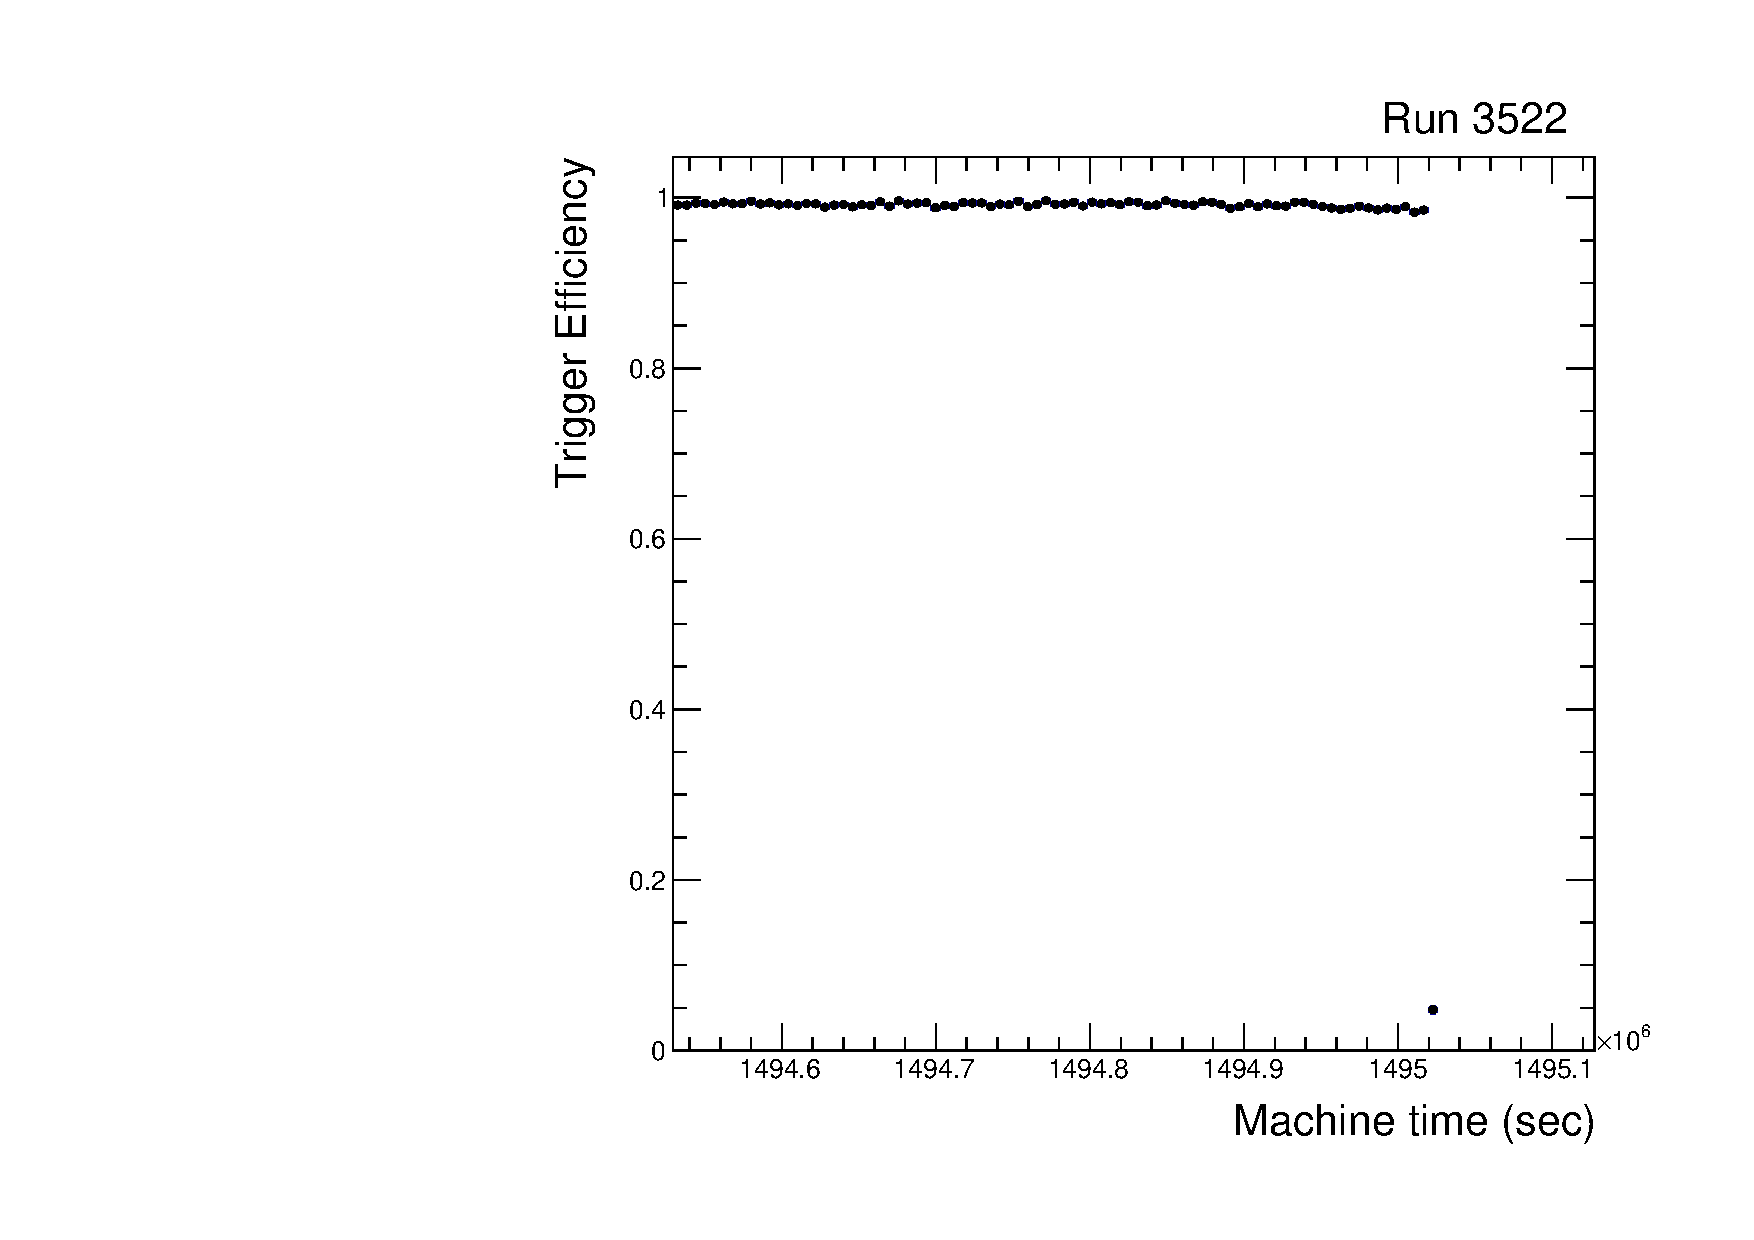
\includegraphics[width=0.48\textwidth]{figures/gbtanalysis3522/tpeff.pdf}
    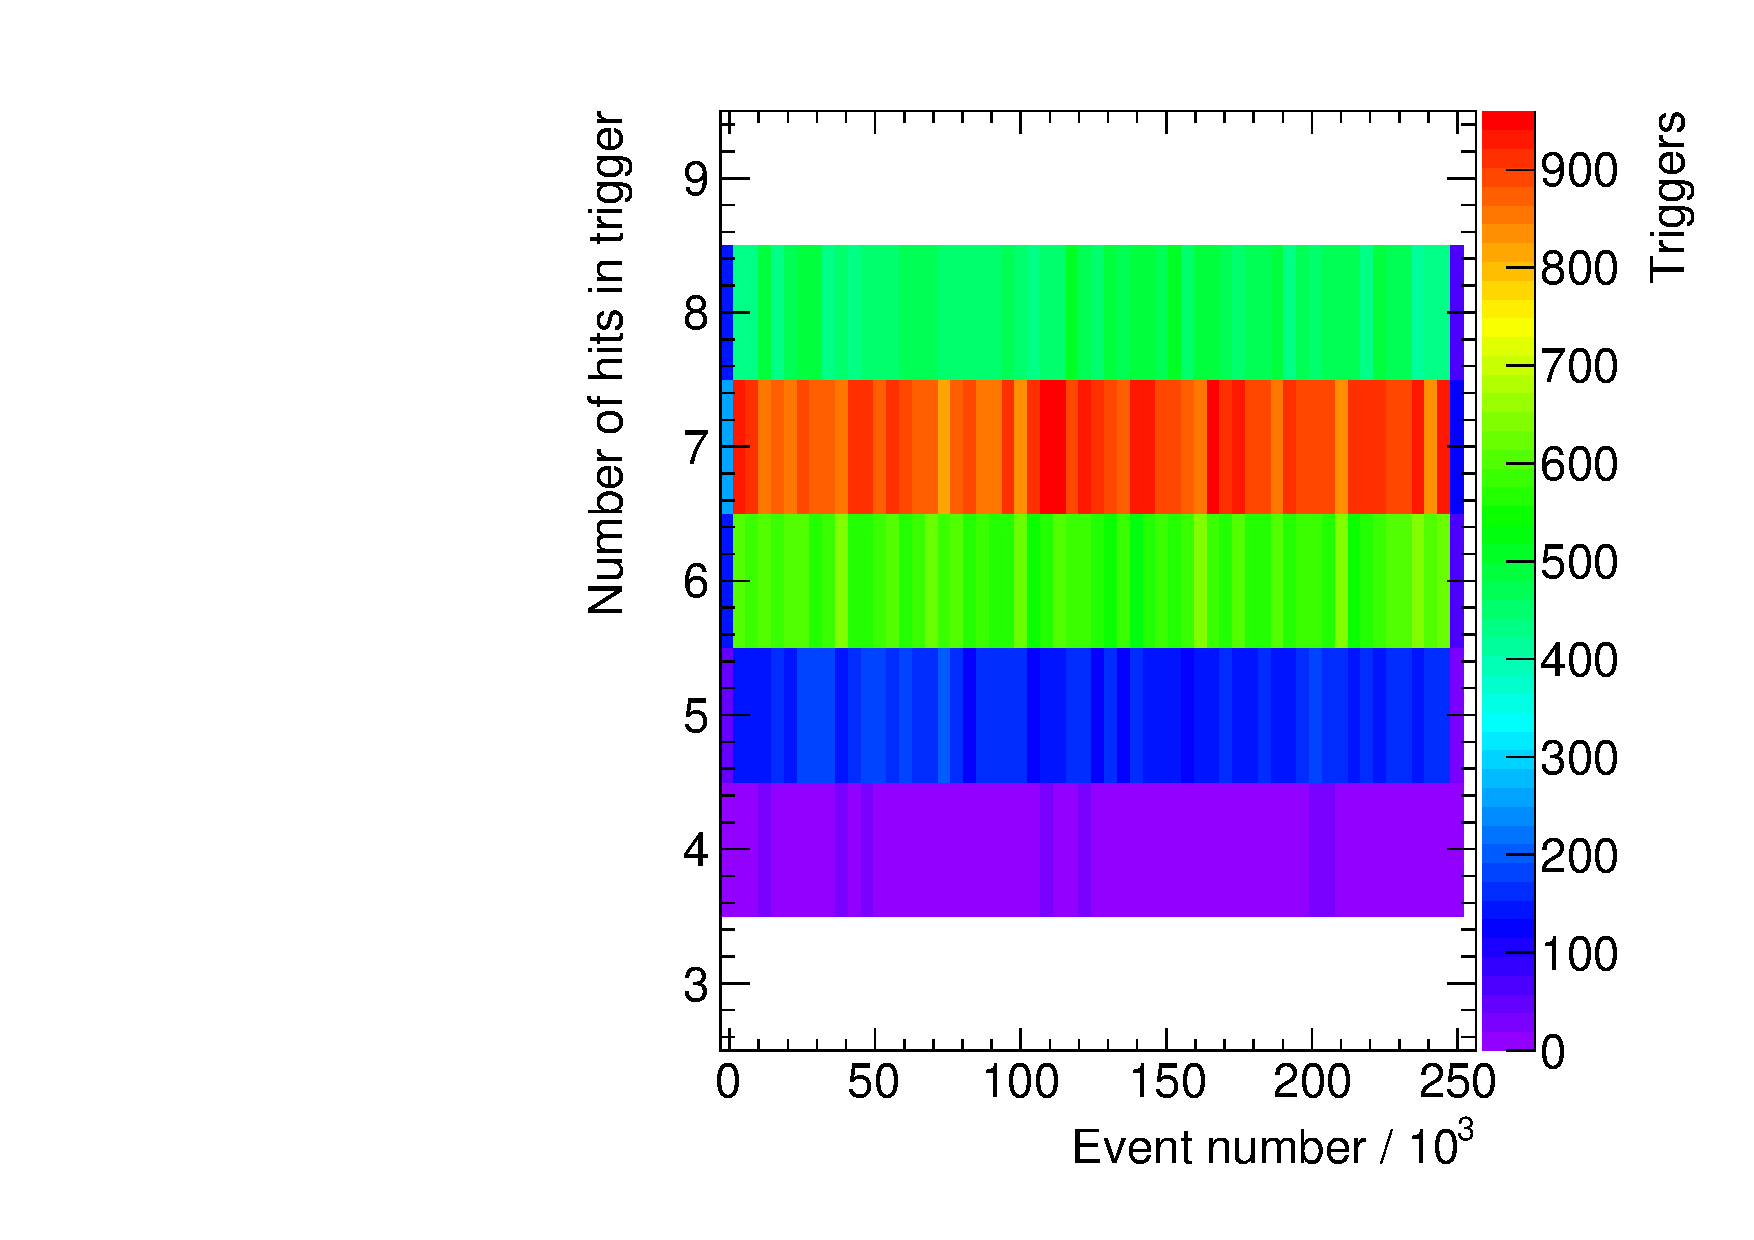
\includegraphics[width=0.48\textwidth]{figures/tuna_analysis/trigger_hits_vs_event.pdf}
  \end{center}
  \vspace{-10pt}
  \caption{MMTP efficiency  (left) and the number of hits producing a trigger (right)
 as a function of time.}
  \label{fig:lowlevel}
\end{figure}
%%%%%%%%%%%%%%%%%%%%%%%%%%
In Fig.~\ref{fig:tp_vs_fe}, we compare the distribution of the muon angles of incidence as measured by the MMTP and offline using MMFE8 clusters, 
as well as the number of MMTP hits and MMFE8 clusters used to reconstruct a muon track. 
As discussed in Sec.~\ref{sec:alg-finder}, the $\simeq $ 0.3\% inefficiencies of the MMTP are due to the 8 BC window used by the finder.


%%%%%%%%%%%%%%%%%%%%%%%%%%%%%%%%%%%%%%%%%%%%%%%%%%
\begin{figure}[!htpb]
  \begin{center}
    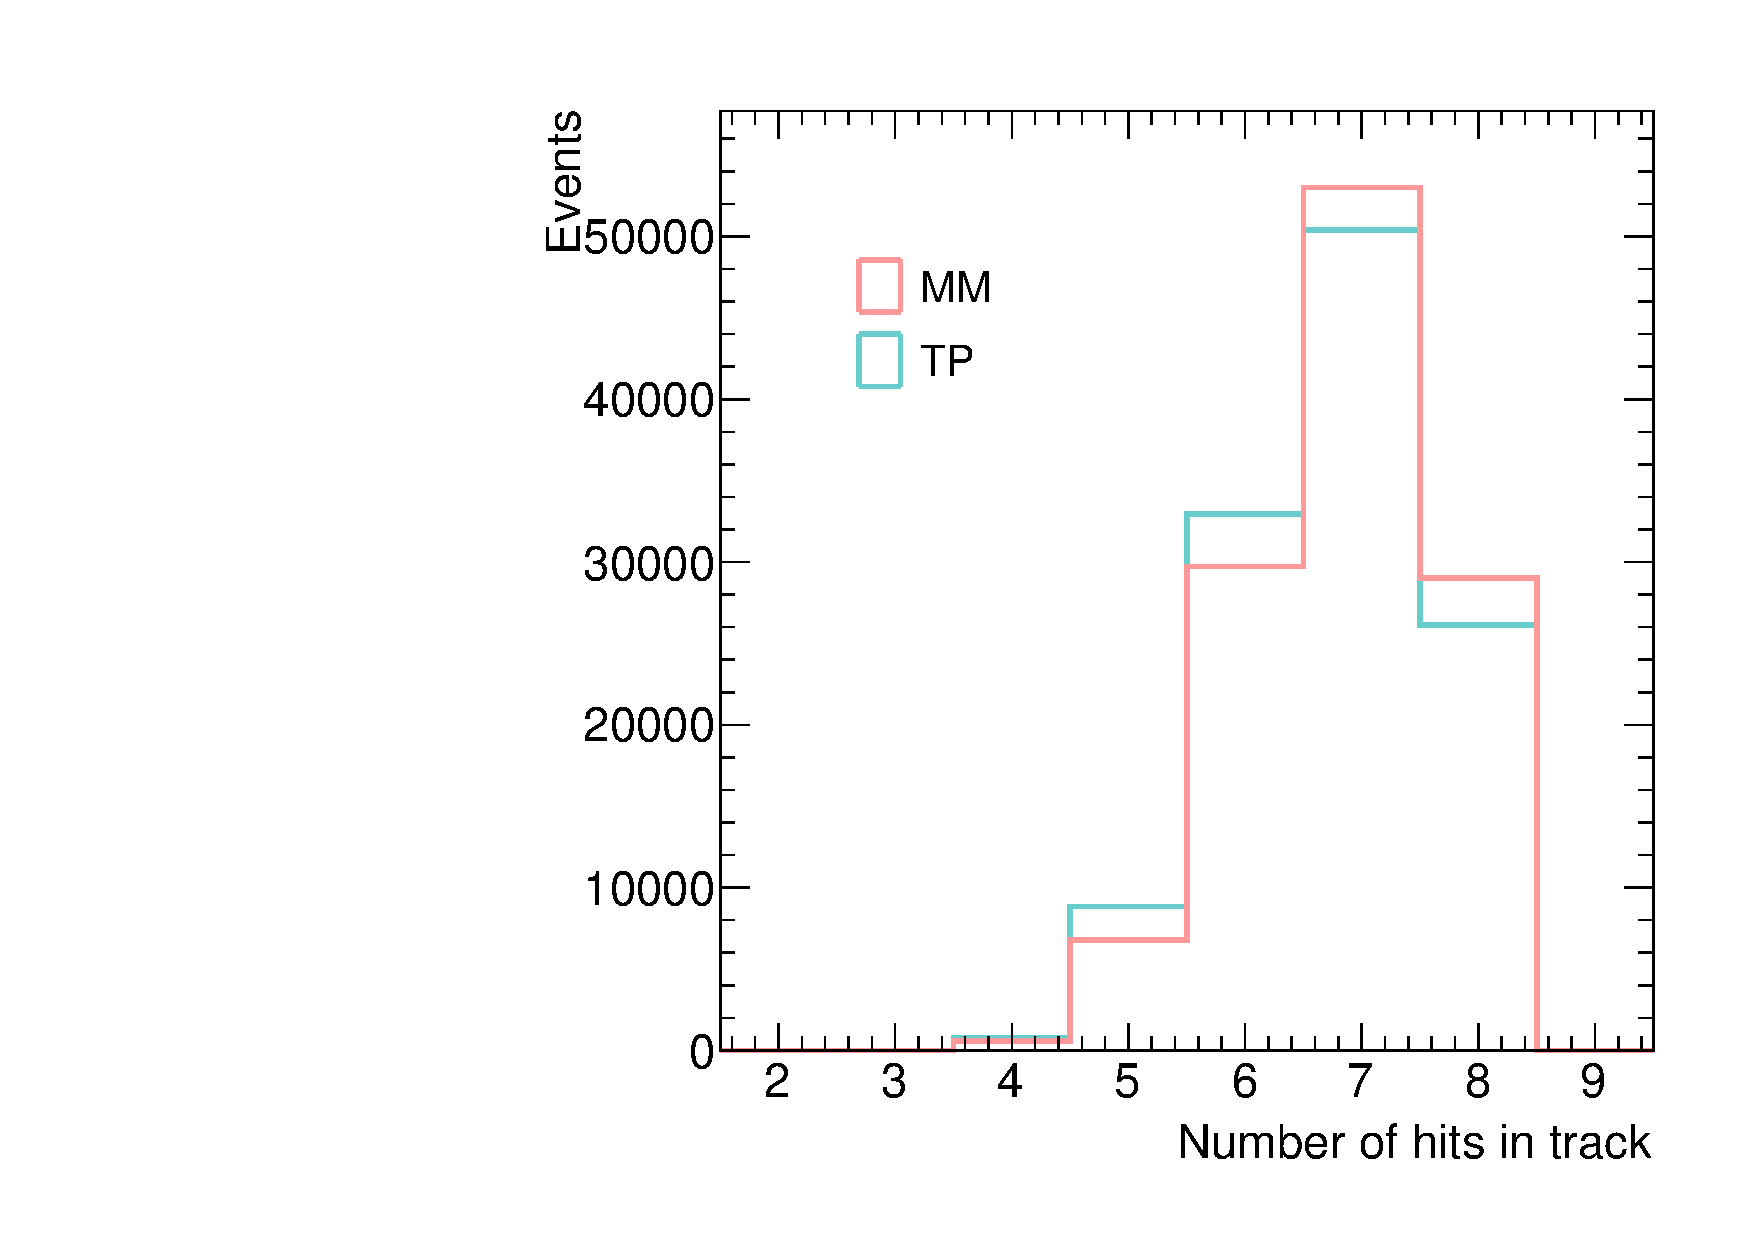
\includegraphics[width=0.48\textwidth]{figures/tuna_analysis/trigger_nart.pdf}
    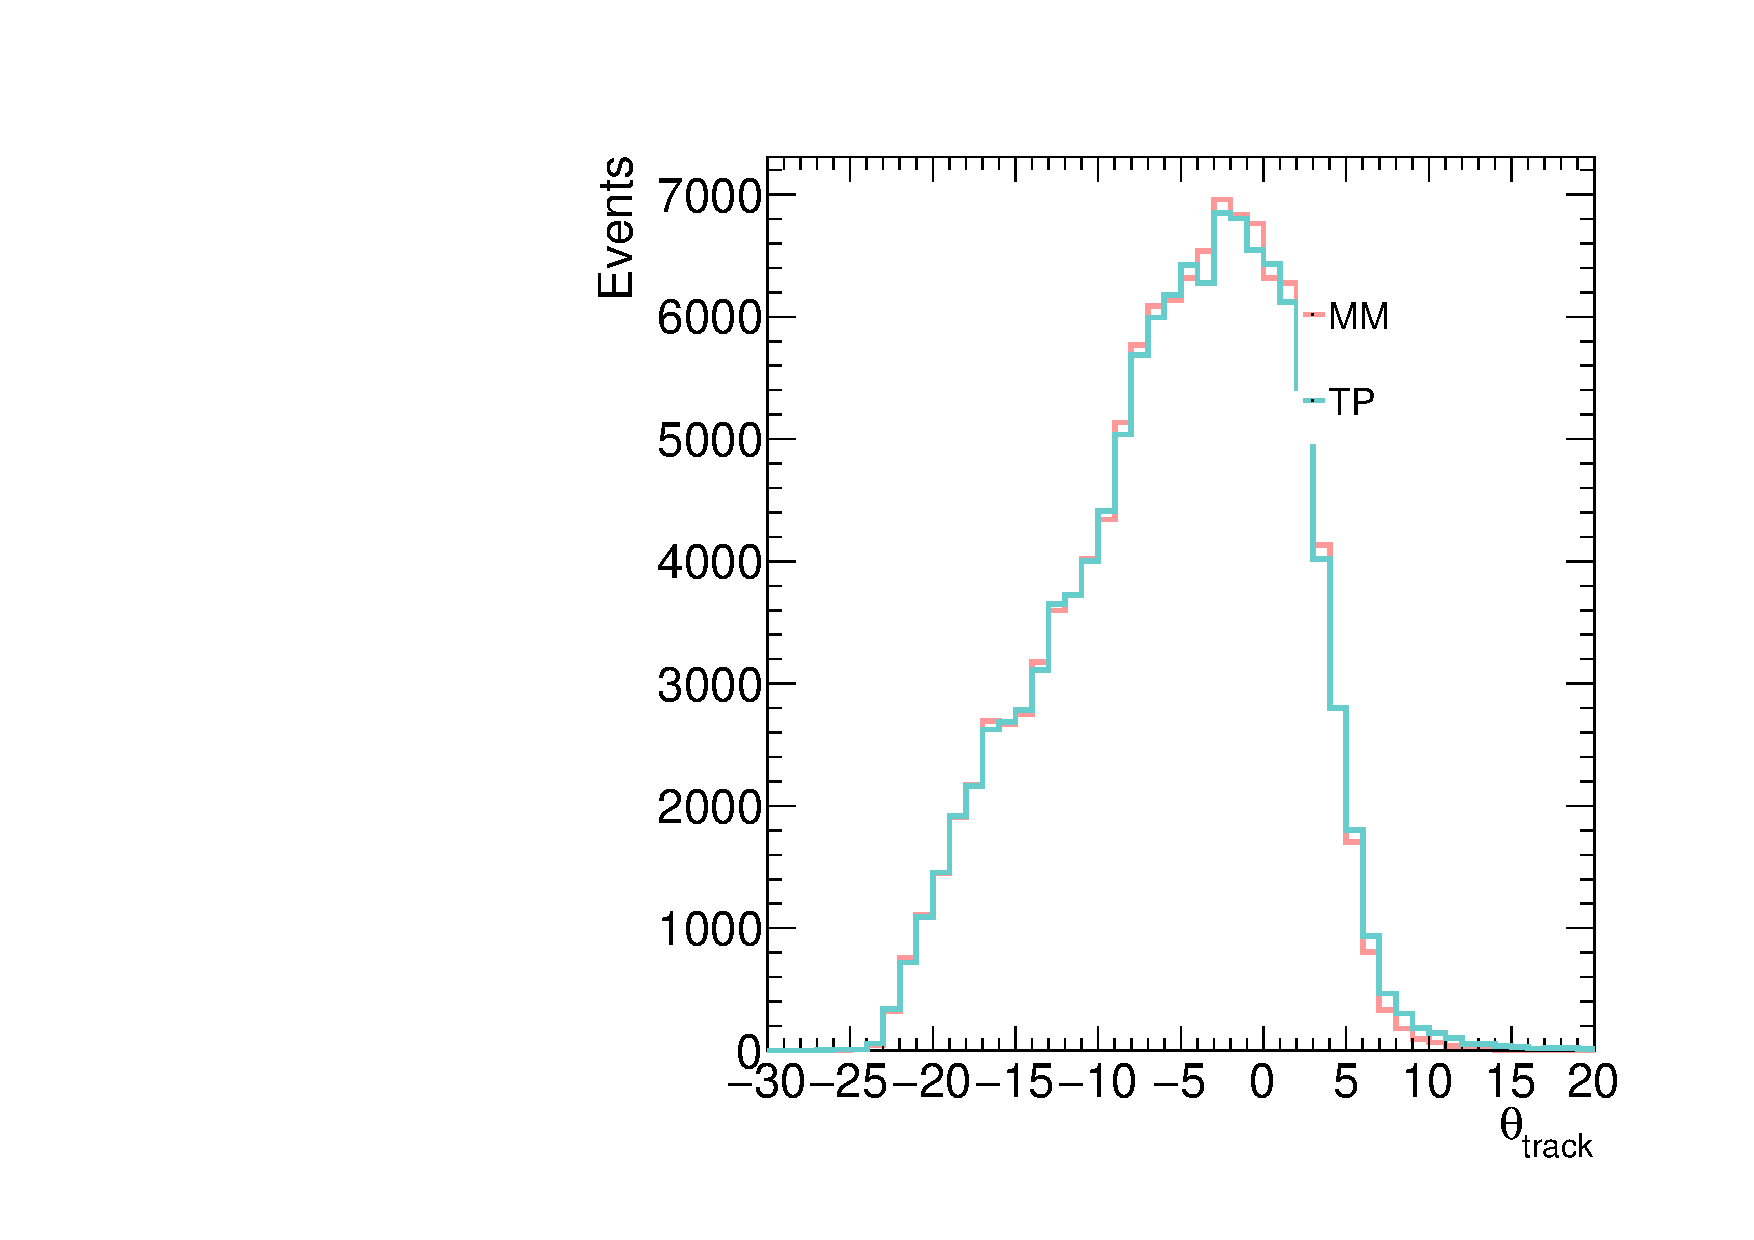
\includegraphics[width=0.48\textwidth]{figures/gbtanalysis3522/ang.pdf}
  \end{center}
  \vspace{-10pt}
  \caption{Distribution of the number of hits and clusters in the MMTP and MM reconstructed tracks (left). 
Distribution of the track's angle reconstructed by the MMTP
 and offline using MM clusters (right).}
  \label{fig:tp_vs_fe}
\end{figure}
%%%%%%%%%%%%%%%%%%%%%%%%%%%%%%%%%%%%%%%%%%%%%%%%%

\subsection{Offline roads}
\label{sec:perf-roads}

In order to cover the angular acceptance of our telecope, the MMTP algorithm uses 1 VMM  roads, and effectively
 3 VMM roads after including neighboring roads. 
Because the rate of ART noise signals issued by each VMM ranges between 100 and 300 Hz, in our case accidentals triggers or accidental hits replacing
good hits of a track are not an issue. In our case, the spatial resolution is largely degraded by $\delta$ rays
 with energies as low as a few KeV, which in $\simeq$ 15\% of the events replace a
correct  ART hit (see Fig.~\ref{fig:deltarays}).

%%%%%%%%%%%%%%%%%
\begin{figure}[!htpb]
  \begin{center}
    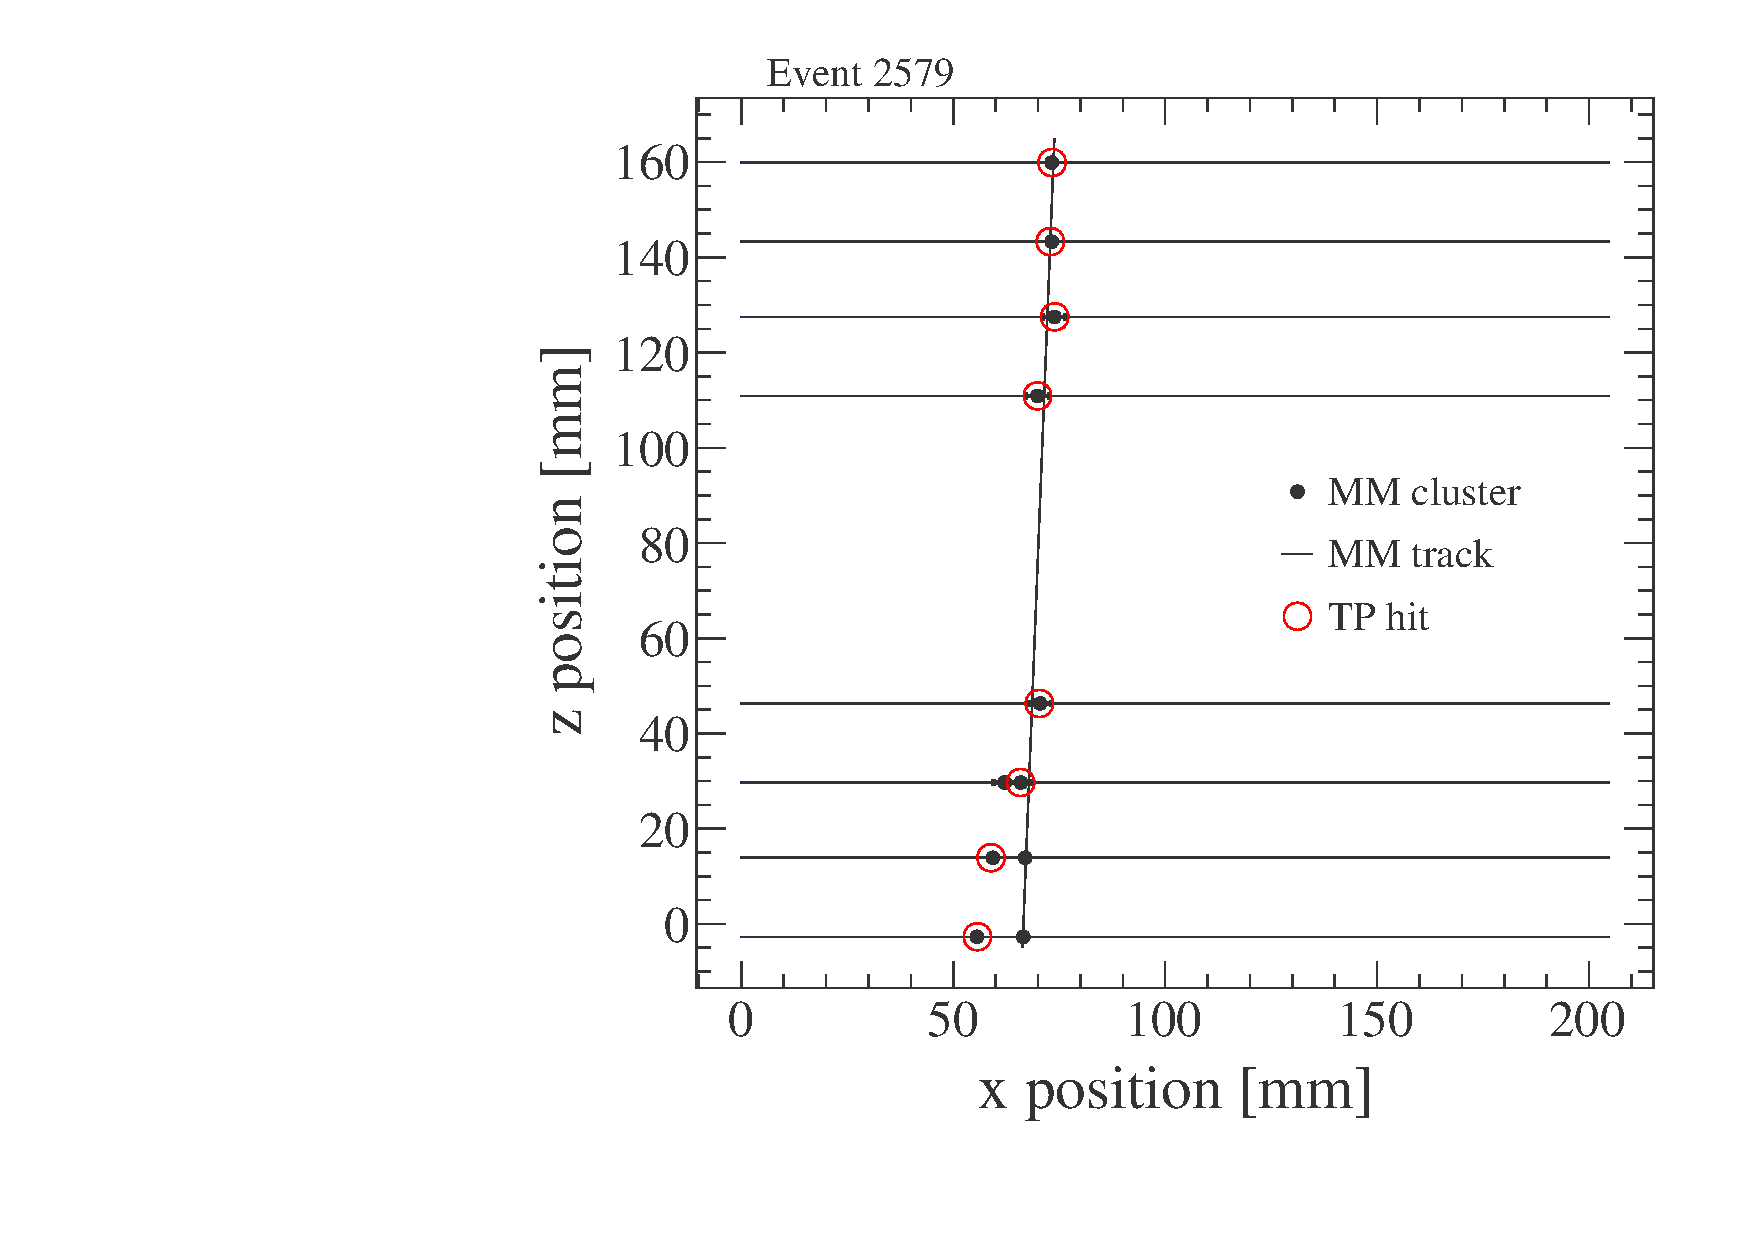
\includegraphics[width=0.48\textwidth]{figures/event_displays/display_02579.pdf}
    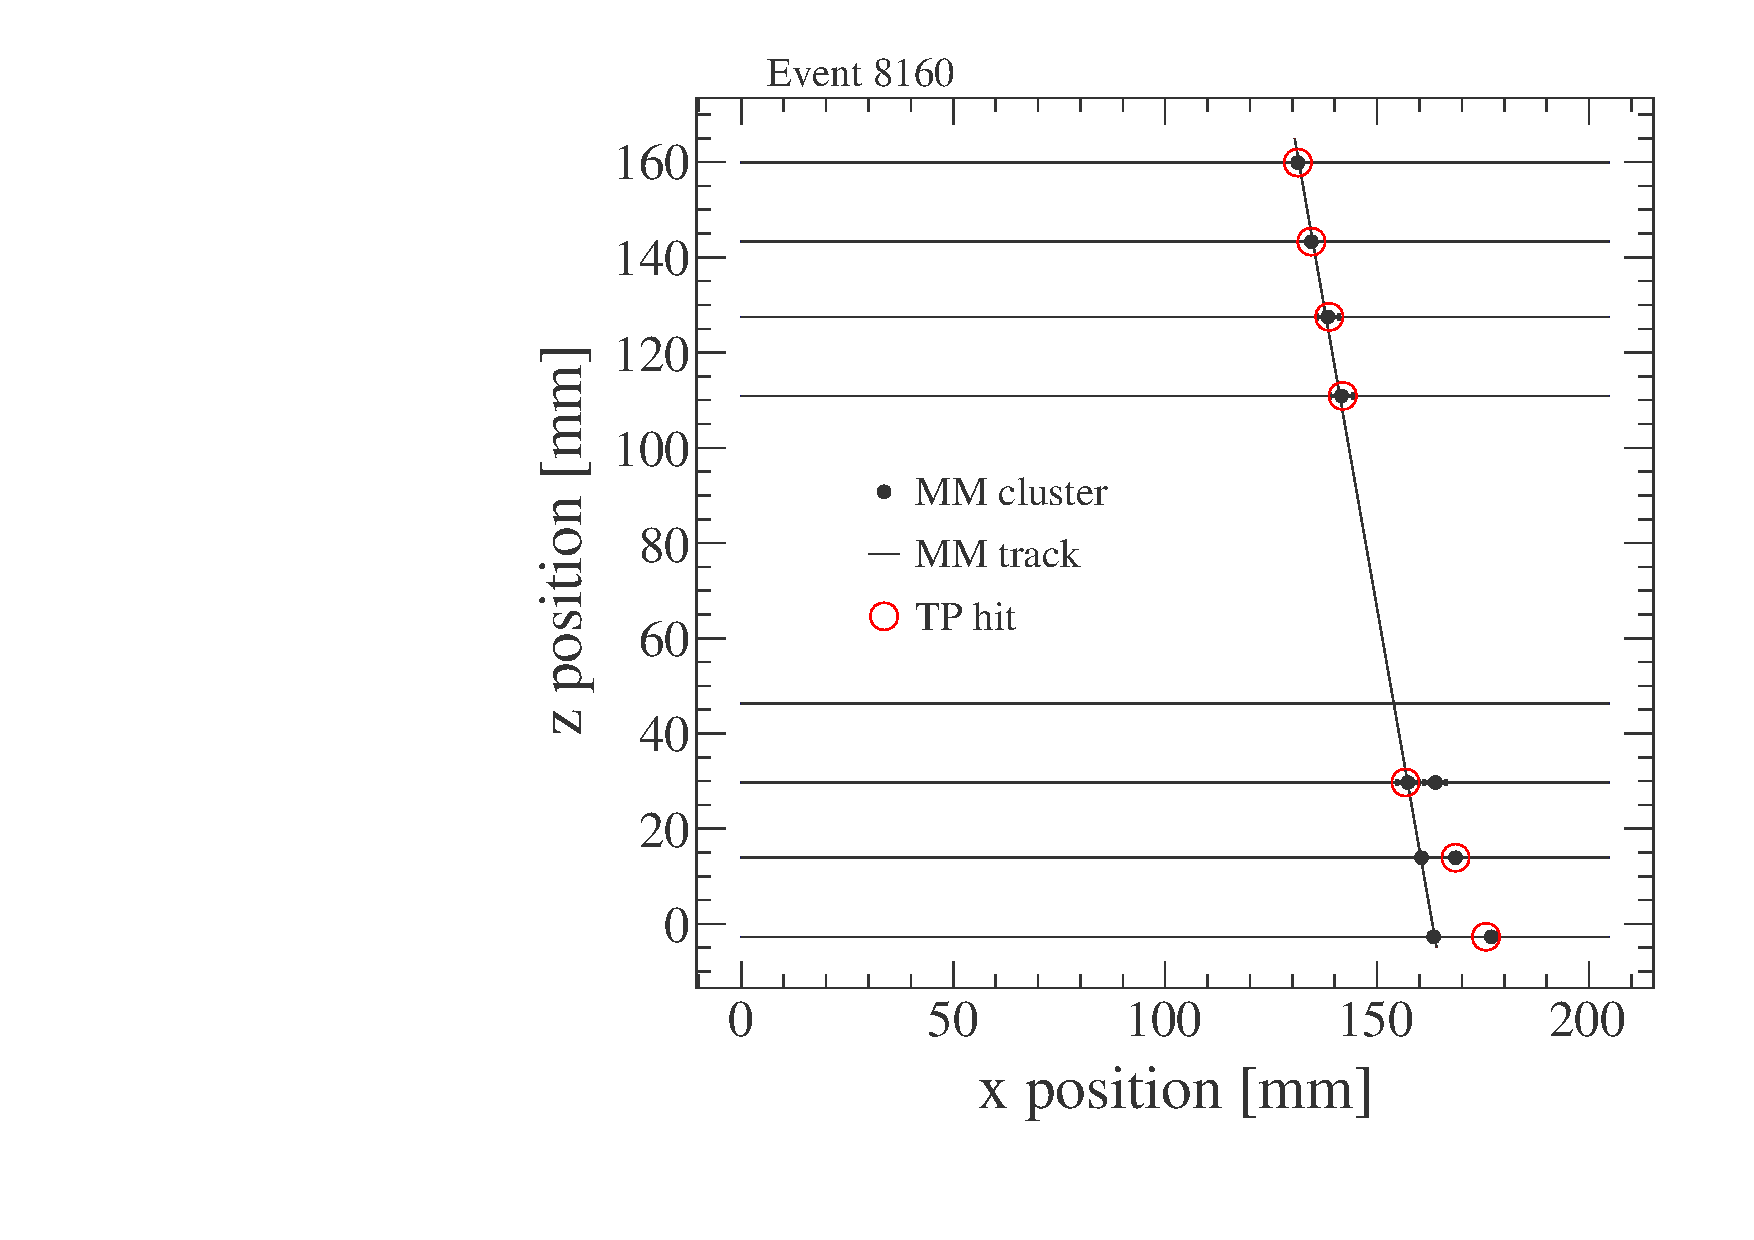
\includegraphics[width=0.48\textwidth]{figures/event_displays/display_08160.pdf}
  \end{center}
  \vspace{-10pt}
  \caption{Display of two events with $\delta$ rays. The black points are MM clusters, 
the black line is the fit to the clusters, and the red circles are the hits chosen by the MMTP. 
We select these events by requiring that the difference between the $\theta$ angles reconstructed by the MMTP and offline 
using MM cluster is larger than 10 mr.}
  \label{fig:deltarays}
\end{figure}
%%%%%%%%%%%%%%%%%%%%%%%%%%%%%%%%%%%%%%%%%%%%%%%%%%%%%%%%
 As the material in front of the NSW detector cannot be less than that in front of our octuplet,  $\delta$ rays will  represent an irreducible source
 of performance degradation.  Of course, this effect is reduced when using smaller roads as is the case for the NSW algorithm which plans to use
 0.9 mr roads for $X$ planes,  corresponding to  1/4 VMM roads for our algorithm. 
 
 For stereo planes, the NSW road size depends on the length of the Micromegas $x$ strips which ranges from 500 to 2200 cm as shown in
 Fig.~\ref{fig:stereo_roads}.
%%%%%%%%%%%%%%%%%%%%%%%%%%%%%
 \begin{figure}[!htpb]
  \begin{center}
    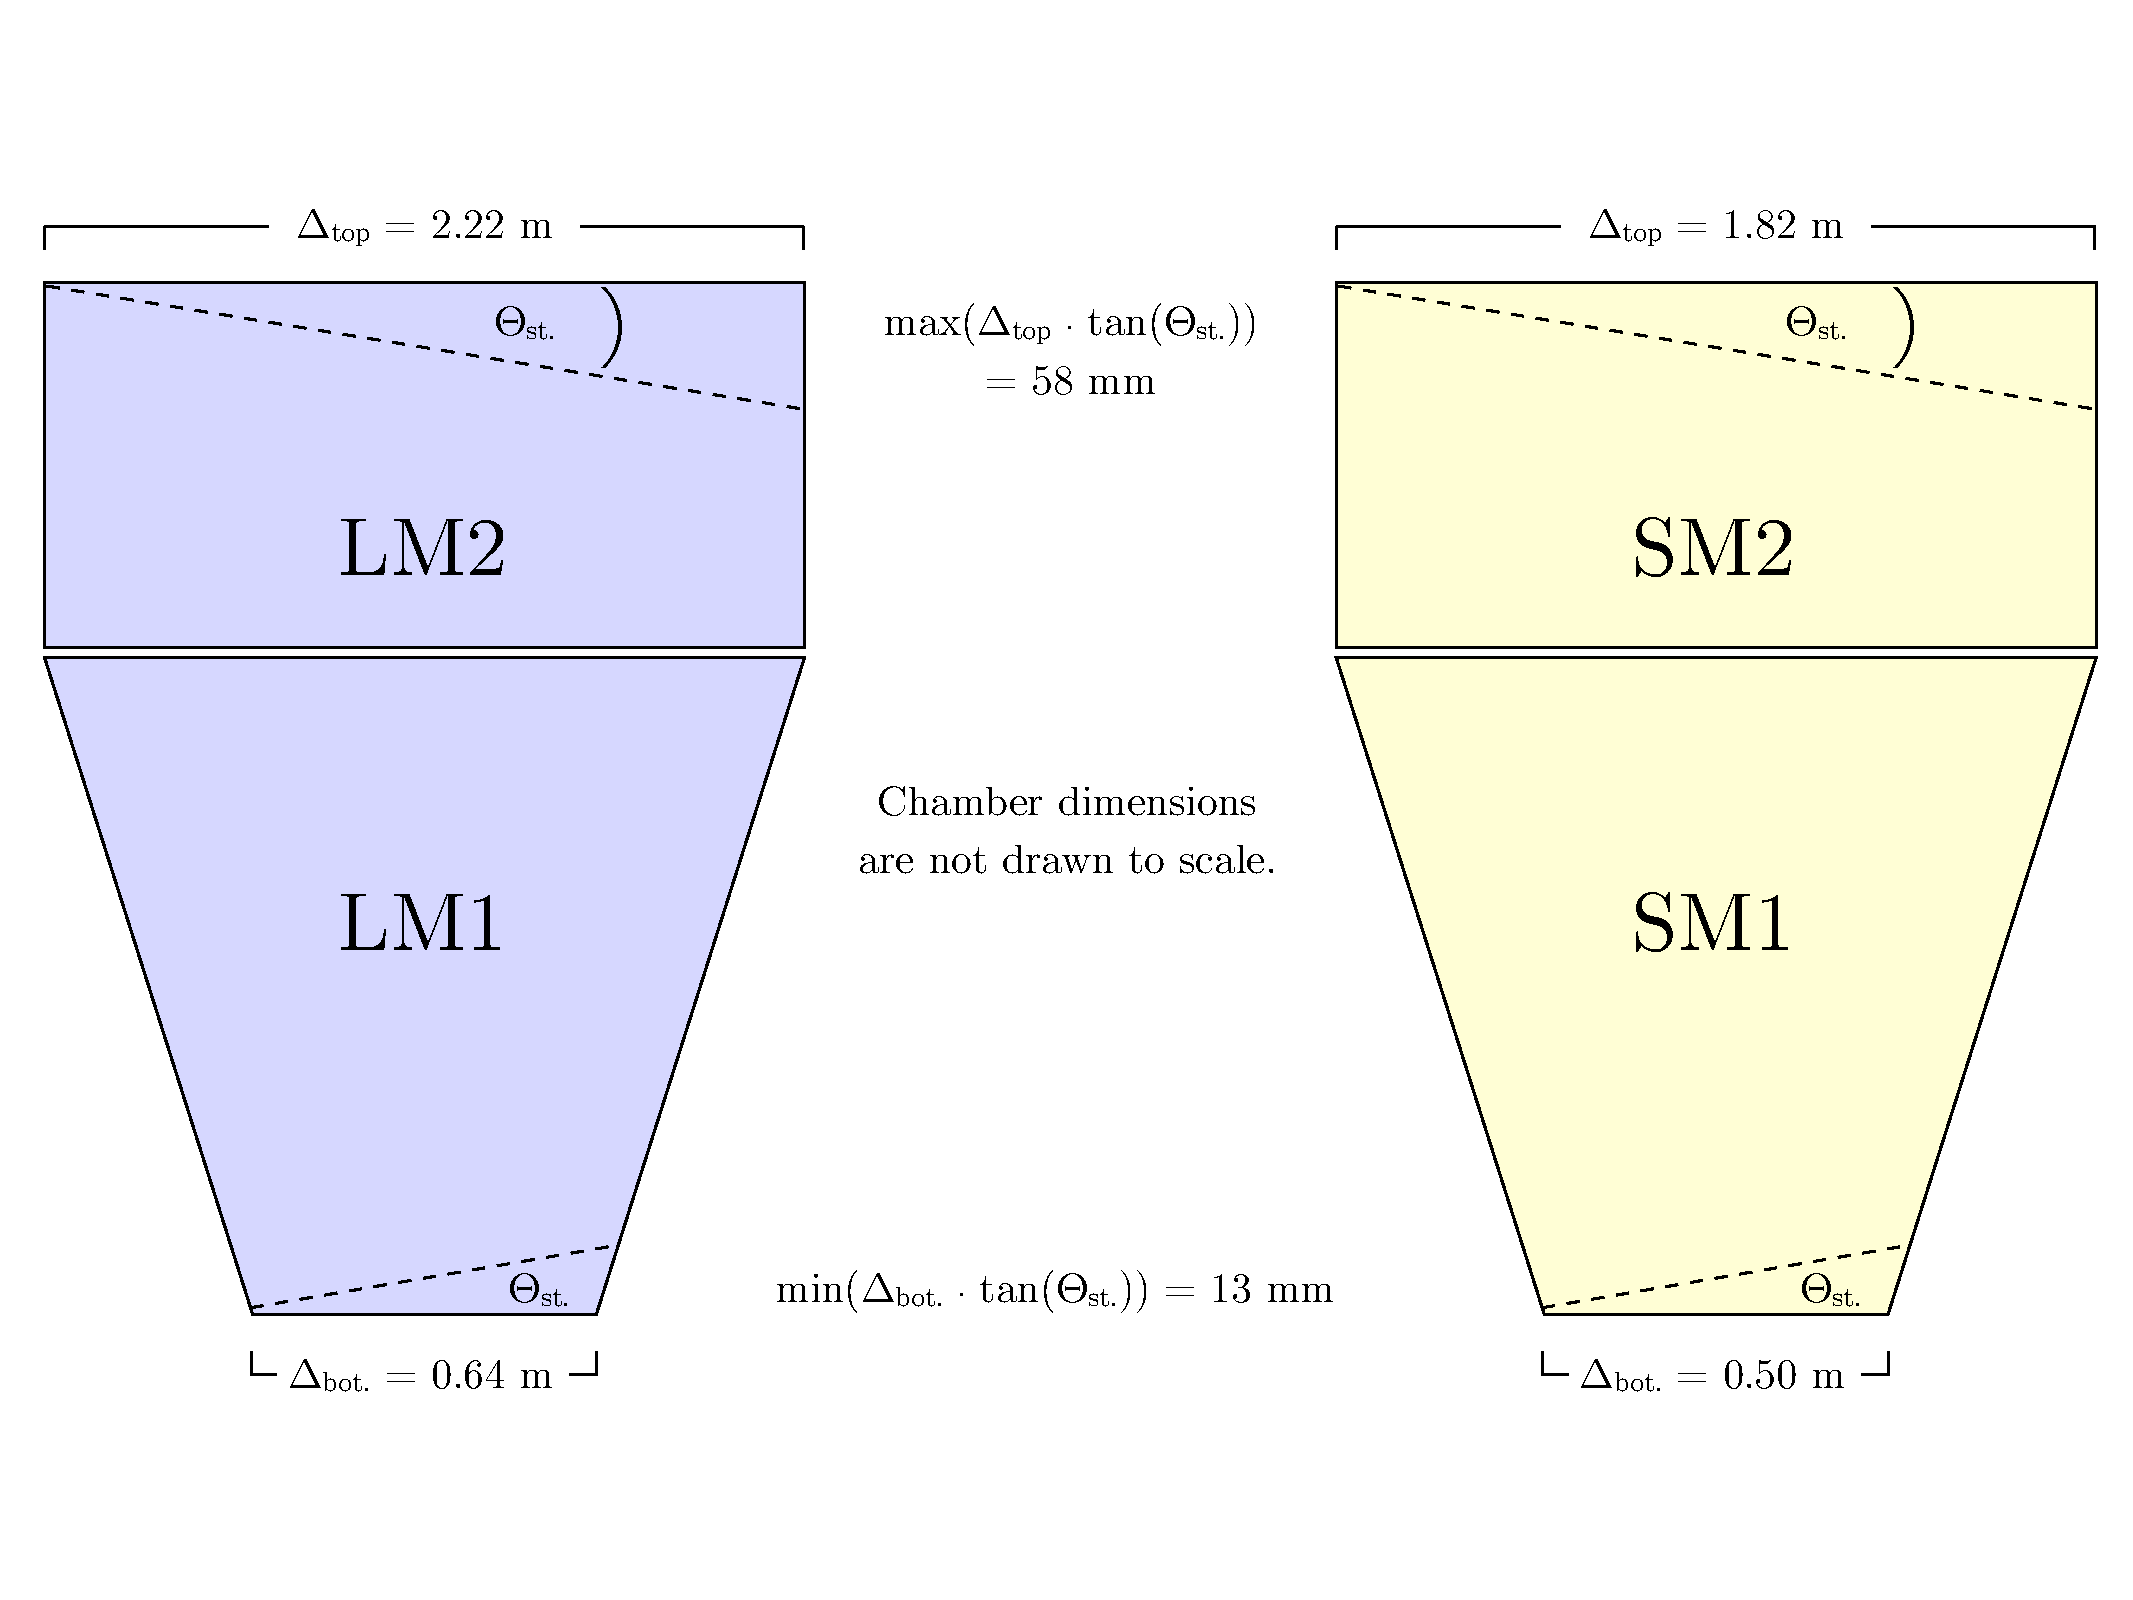
\includegraphics[width=1.0\textwidth]{figures/cartoons/stereo_roads.pdf}
  \end{center}
  \vspace{-10pt}
  \caption{Drawings of  Micromegas wedges with  dimensions as specified by the NSW TDR. The stereo strips require larger roads than the horizontal strips because they 
overlap a band of $x$ strips of width from  13 to 58 mm.}
  \label{fig:stereo_roads}
\end{figure}
 %%%%%%%%%%%%%%%%%%%%%%%%%%%%%%%%%%%%%%%%%%%
For the shortest and longest readout strips, stereo roads need  additional 13 mm (or 32 strips) and 58 mm (144 strips) to cover just one $x$ strip, respectively.
In the following, we first show resolutions using 1 VMM roads with neighbor roads. Then, we emulate the NSW roads using the 
track direction provided by fitting MM cluster.
For $X$ planes, the offline finder uses only ART hits which are at a distance of $\pm$ 24 strips from the intersection of the track with the plane (three 1/4 VMM roads).
For $U,V$ planes, the road is increased by 32 up to 144 strips. The latter increase brings the road width back to the 3 VMMs required online.  
These $X$ and stereo roads emulating the NSW algorithm will be referred to as XNSW, SNSW,  LNSW in the following.
%\end{document}
\subsection{Spatial and angular resolution}
\label{sec:perf-res}
Figures~\ref{fig:xres} to~\ref{fig:yres} show the  $x_{\rm TP}-x_{\rm MM}$ and $y_{\rm TP}-y_{\rm MM}$  distributions
derived with the method in Sec.~\ref{sec:alg-resol}, respectively.
%%%%%%%%%%%%%%%%%%%%%%%%%%%%%%%%%%%%%%%
\begin{figure}[!htpb]
  \begin{center}
    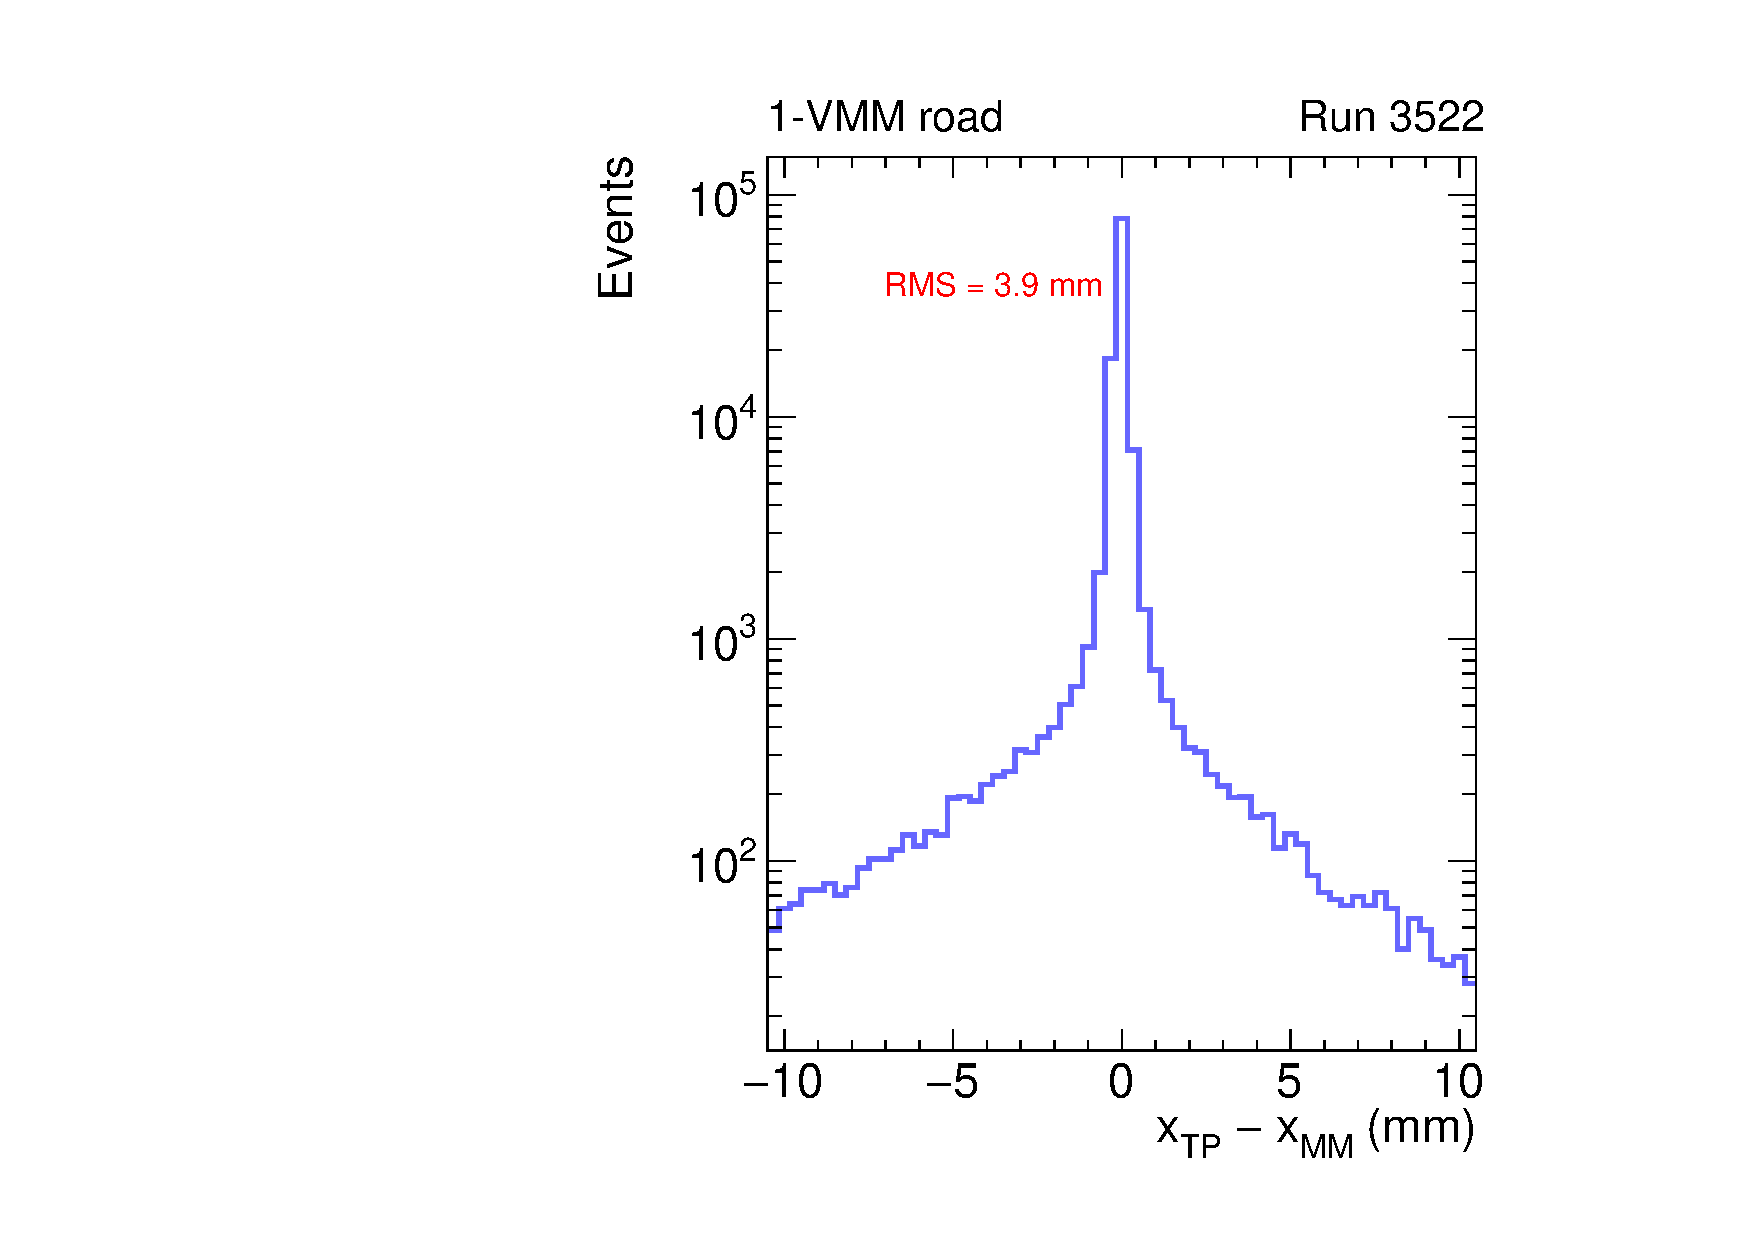
\includegraphics[width=0.48\textwidth]{figures/gbtanalysis3522/TP_xres_full.pdf}
    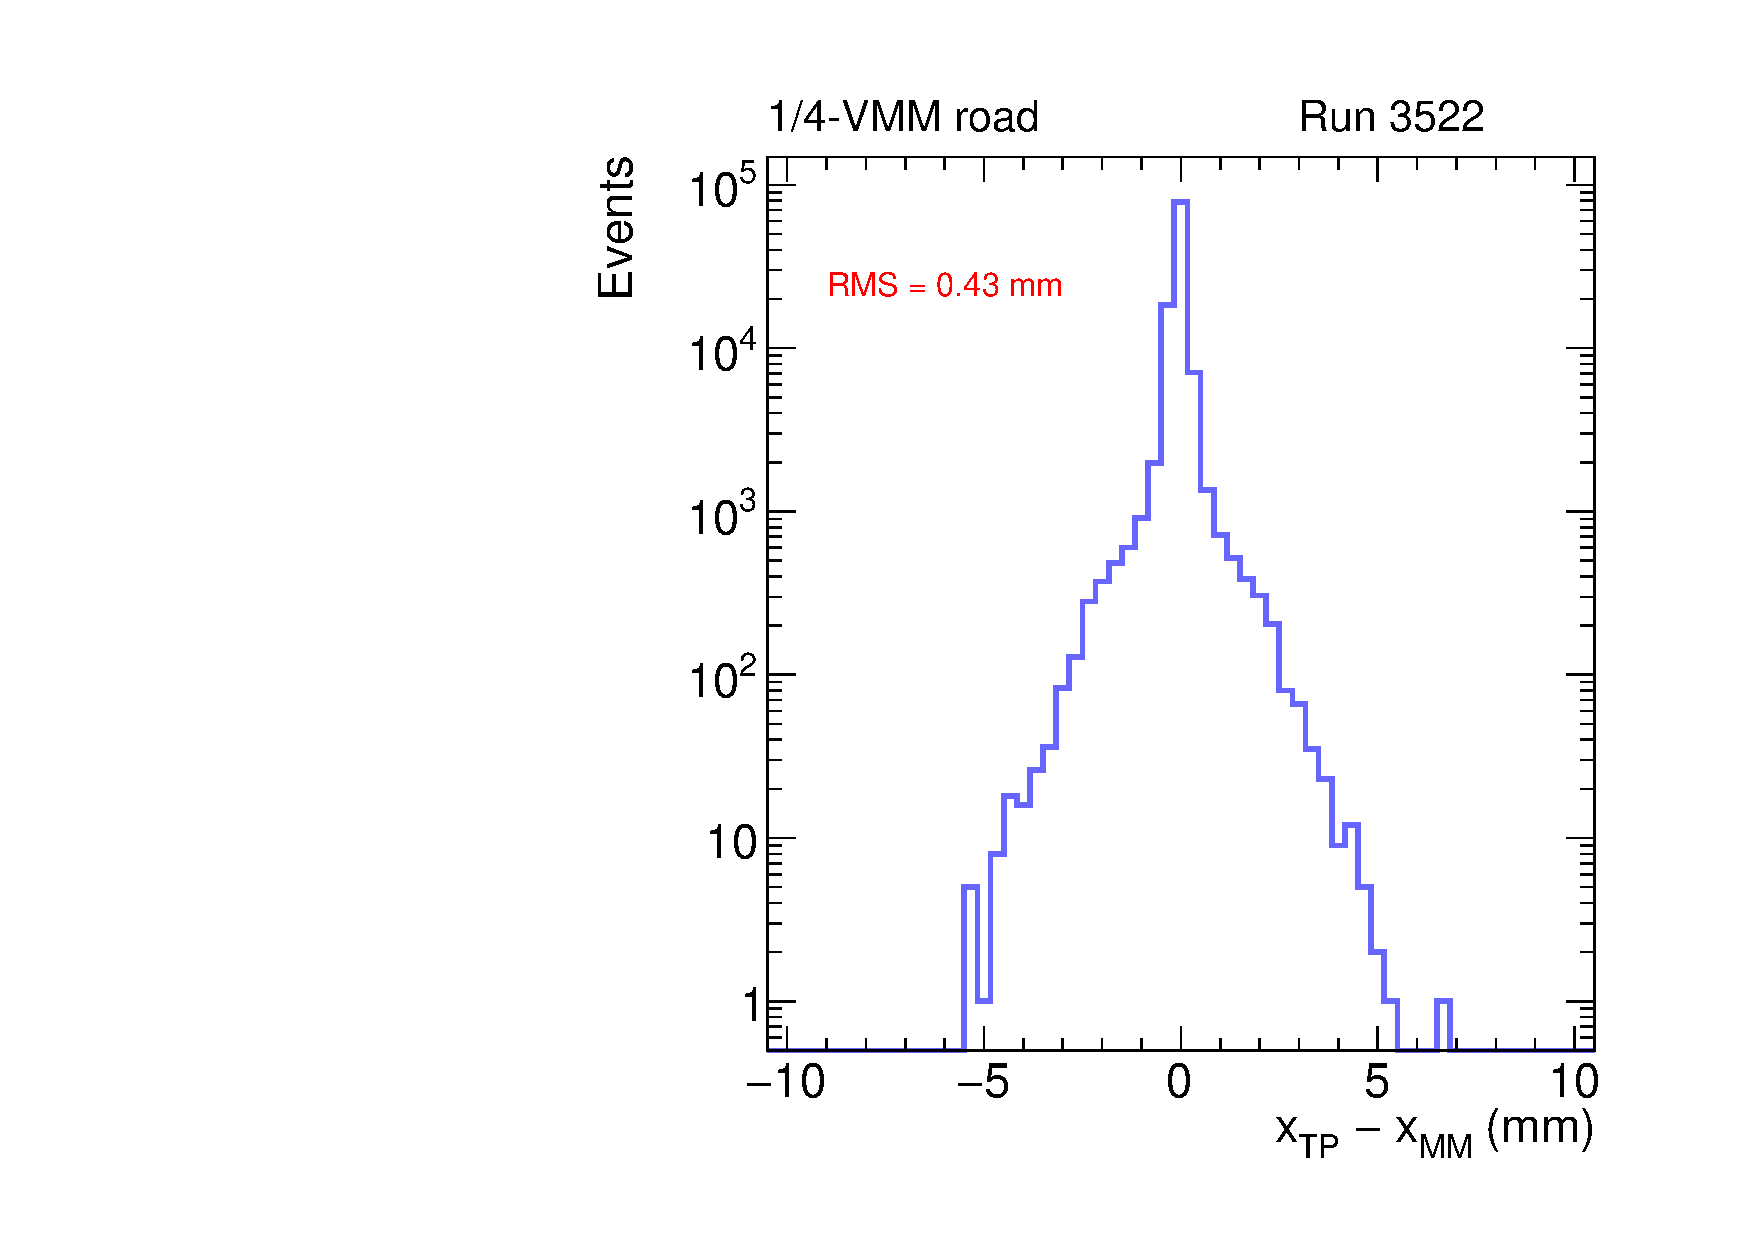
\includegraphics[width=0.48\textwidth]{figures/gbtanalysis3522/TP_xres.pdf}
  \end{center}
  \vspace{-10pt}
  \caption{Distributions of $x_{\rm TP}-x_{\rm MM}$  using (left) 1 VMM roads and (right) XNSW
 roads (see text).}
  \label{fig:xres}
\end{figure}
%%%%%%%%%%%%%%%%%%%%%%%%%%%%%%%%%%%%%%%%%%%
\begin{figure}[!htpb]
  \begin{center}
    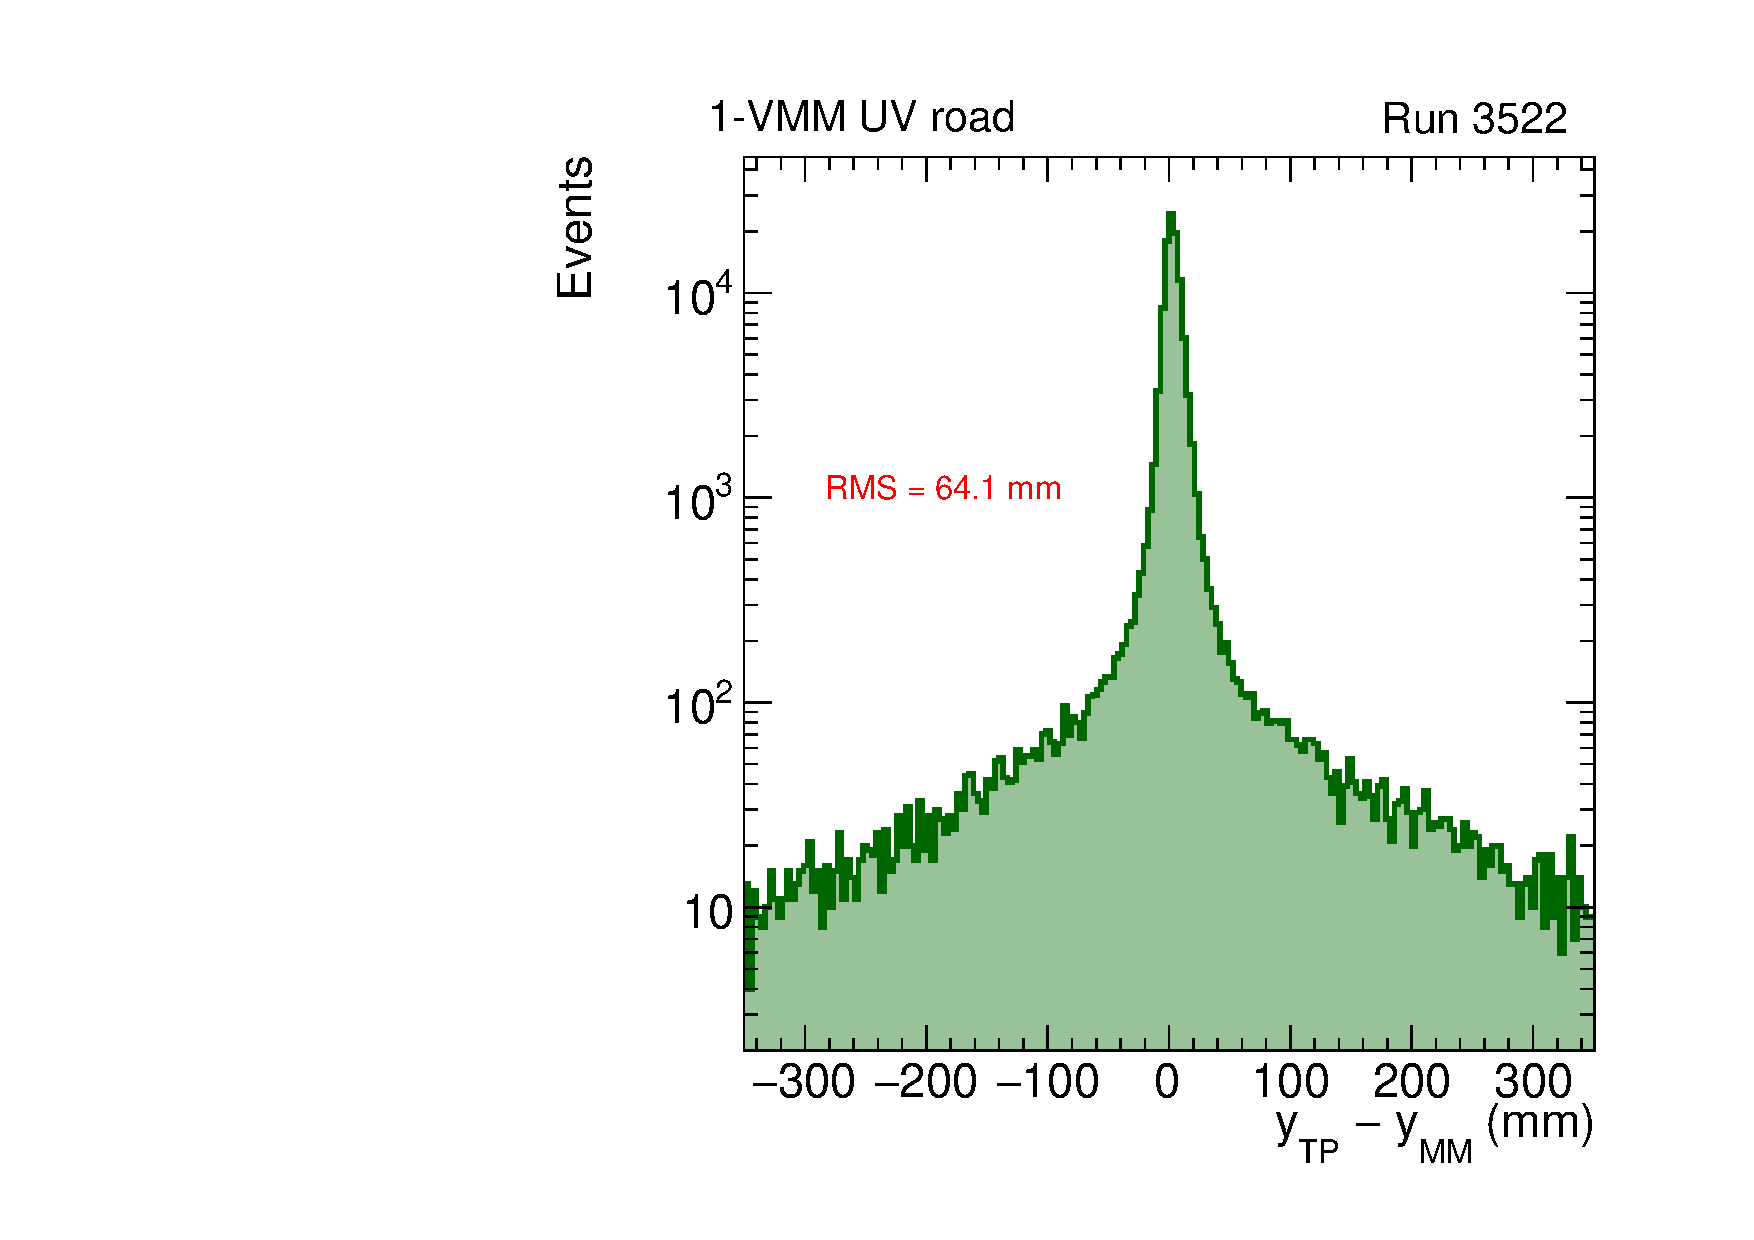
\includegraphics[width=0.48\textwidth]{figures/gbtanalysis3522/TP_yres_1road.pdf}
    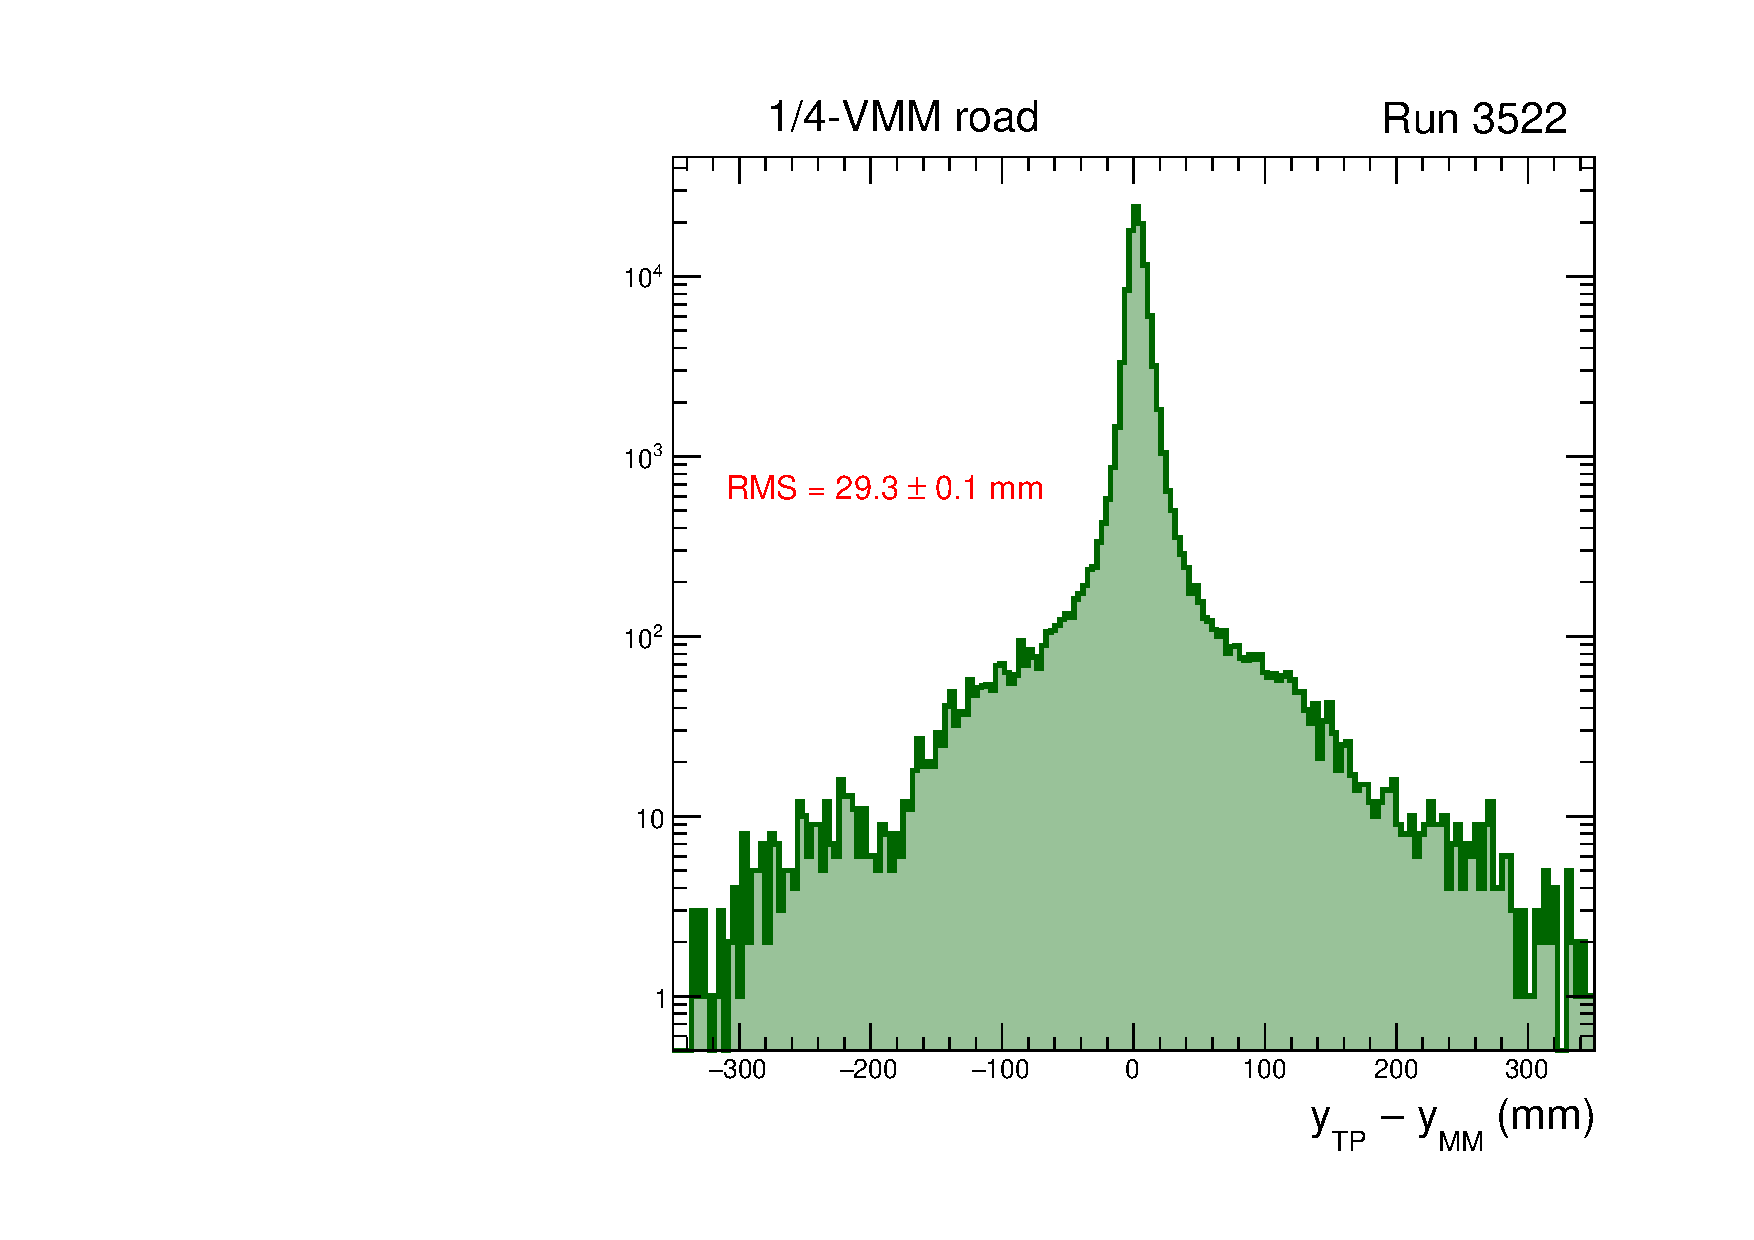
\includegraphics[width=0.48\textwidth]{figures/gbtanalysis3522/TP_yres_smallroad.pdf}
  \end{center}
  \vspace{-10pt}
  \caption{Distributions of $y_{\rm TP}-y_{\rm MM}$  using (left) 1 VMM or LNSW roads 
 and (right) SNSW roads (see text).}
  \label{fig:yres}
\end{figure}
%%%%%%%%%%%%%%%%%%%%%%%%%%%%%%%%%%%%%%%%%%%%%%%%%%%%%%%%%%%%%%

 As expected, the large tails of the above distribution shrink with the road width.
 The global angle resolution 0.43 mm/7.5 m = 0.06 mr is better than what required by the NSW TDR.
  The $y$ resolution segments at $\pm 1 \sigma$ level the shortest  SM1 detector into 8  $\phi $ sectors and the longest LM2 detector
 into 17 $\phi $ sectors. 


 The distribution of $\theta_{\rm local}-\theta_{\rm MM} $ is plotted in Fig.~\ref{fig:thetares}.
The correlation between angular and spatial resolution is shown by Fig.~\ref{fig:xthetares}.
 The NSW TDR  calls for a 15 mr cut on the difference between  the global and local angles.
 Because of $\delta$ rays, this cut  loses at least 4\% of good triggers. 
  At the highest LHC luminosities, the rate per Micromegas strip is anticipated to be 
 as large as 50 kHz per strip, almost independent on the distance from the beamline.
 It seems plausible that accidental hits due to single rates will cause an even higher inefficiency of the
 MMTP trigger if the $\Delta\theta$ cut is implemented.
%%%%%%%%%%%%%%%%%%%%%%%%%%%%%%%%%%%%%%%%%%
\begin{figure}[!htpb]
  \begin{center}
    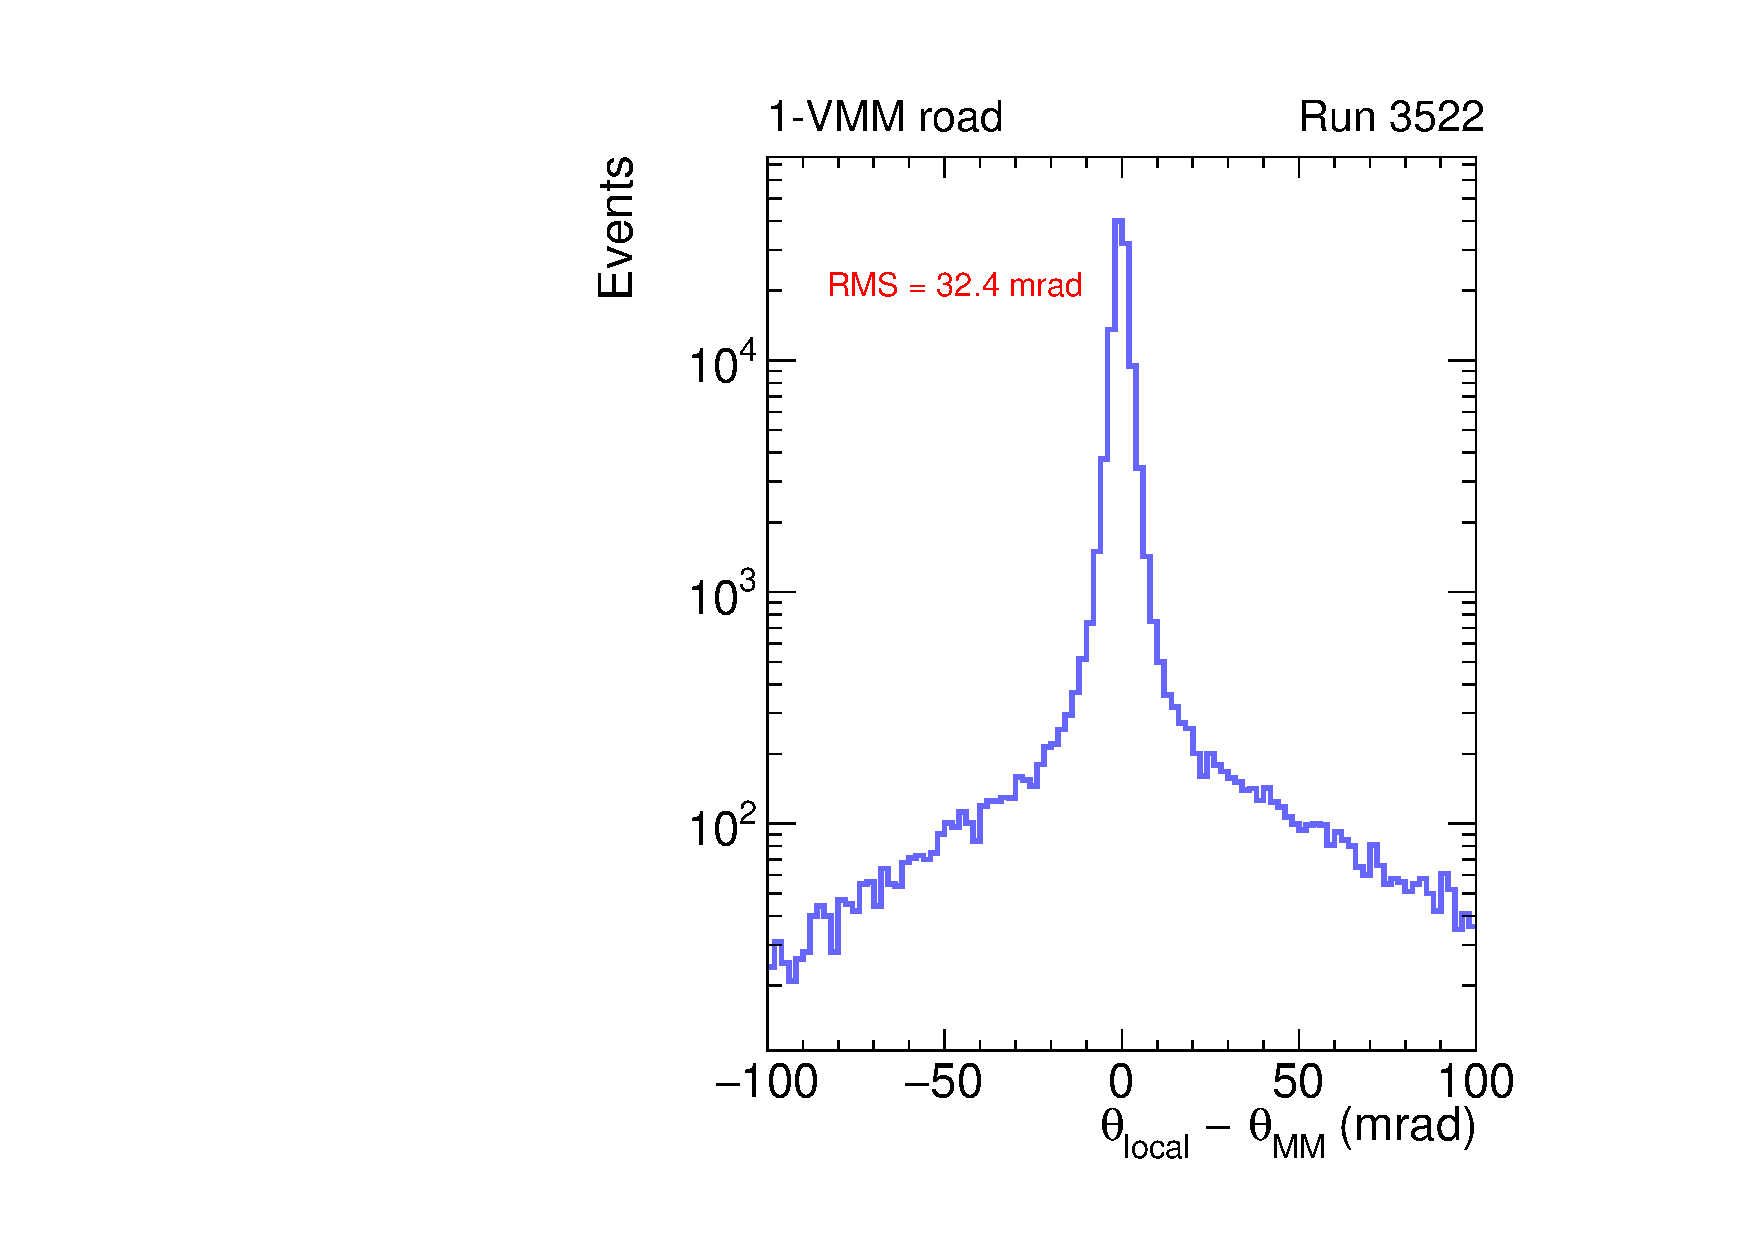
\includegraphics[width=0.48\textwidth]{figures/gbtanalysis3522/TP_angres_full.pdf}
    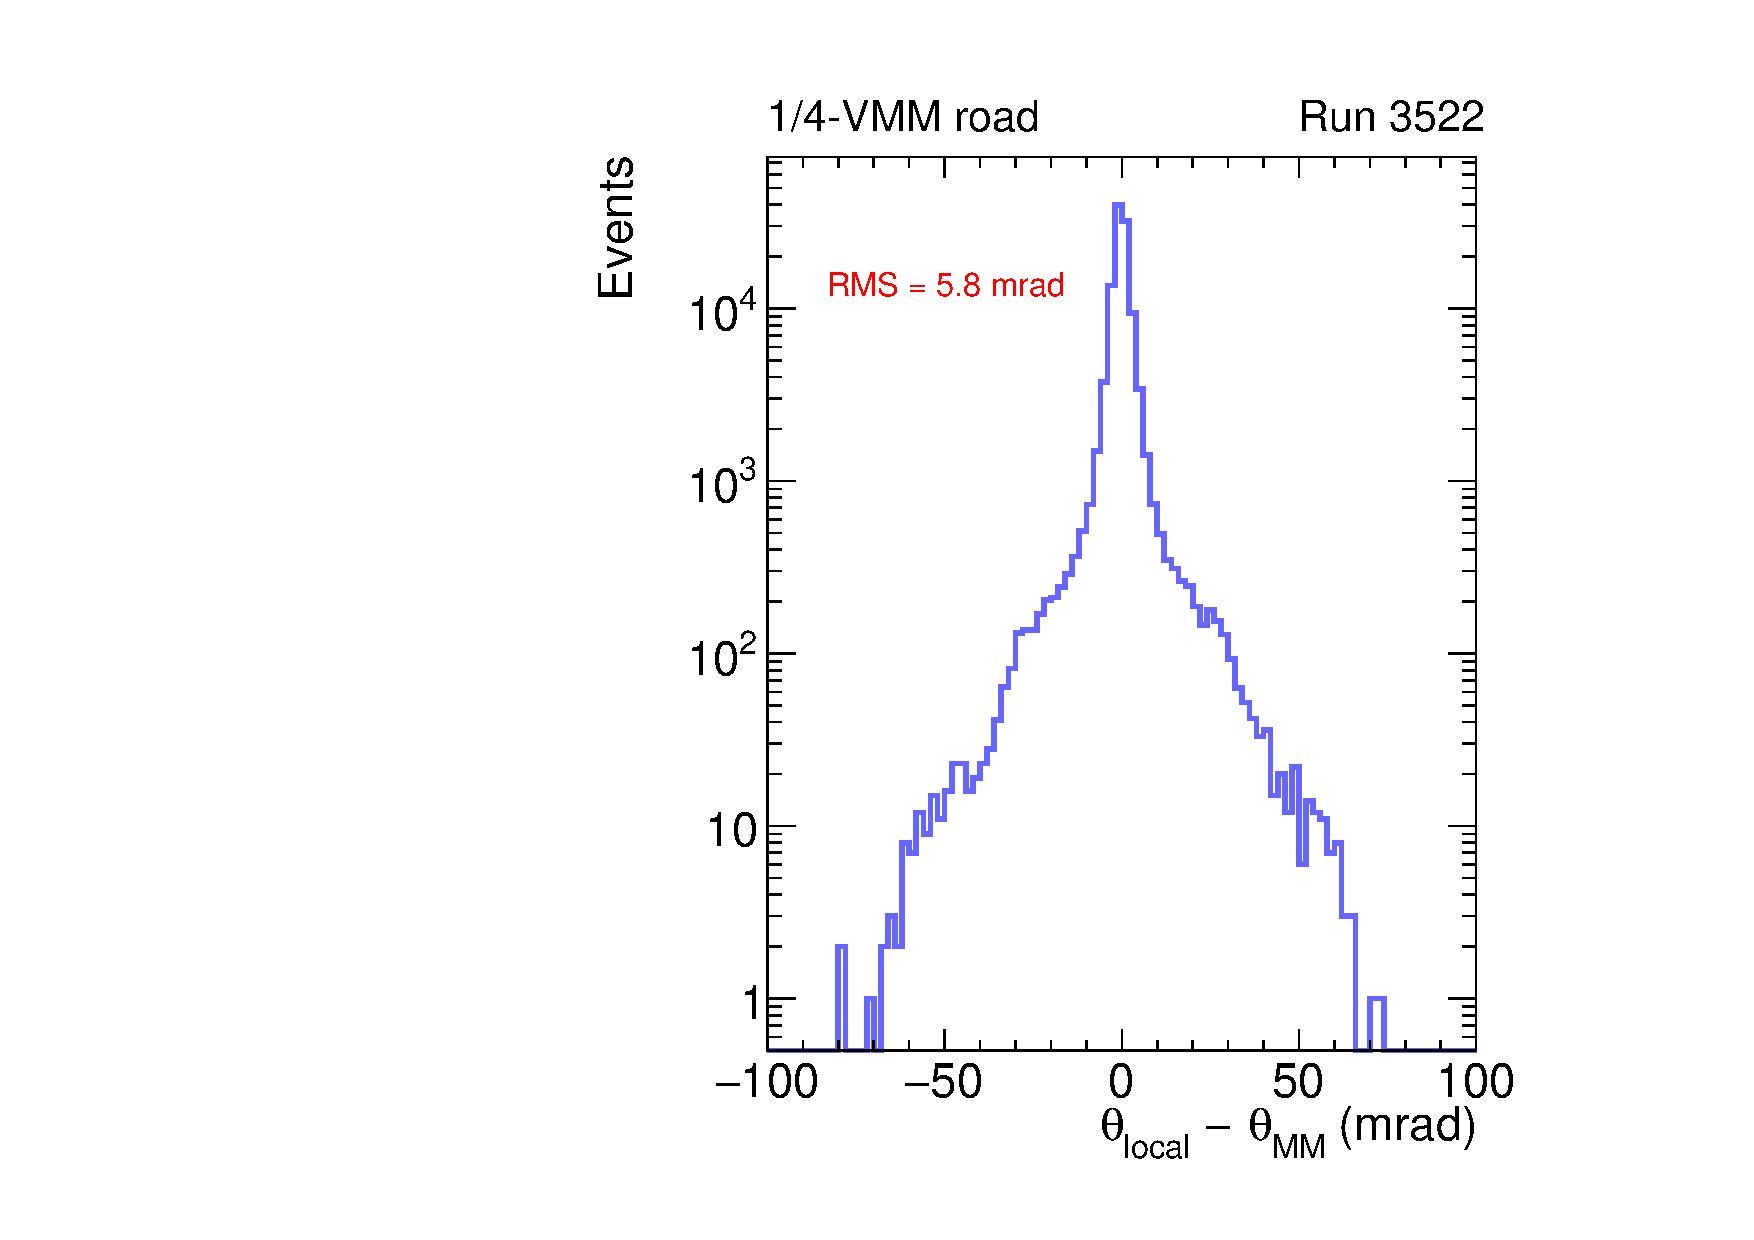
\includegraphics[width=0.48\textwidth]{figures/gbtanalysis3522/TP_angres.pdf}
  \end{center}
  \vspace{-10pt}
  \caption{Distribution of  $\theta_{\rm local}-\theta_{\rm MM} $ using  (left) 1VMM    and (right) XNSW  roads (see text). }
  \label{fig:thetares}
\end{figure}
%%%%%%%%%%%%%%%%%%%%%%%%%%%%%%%%%%%%%%%%%%%%%%%%%%%%%%%%%%%%%%%%
\begin{figure}[!htpb]
  \begin{center}
    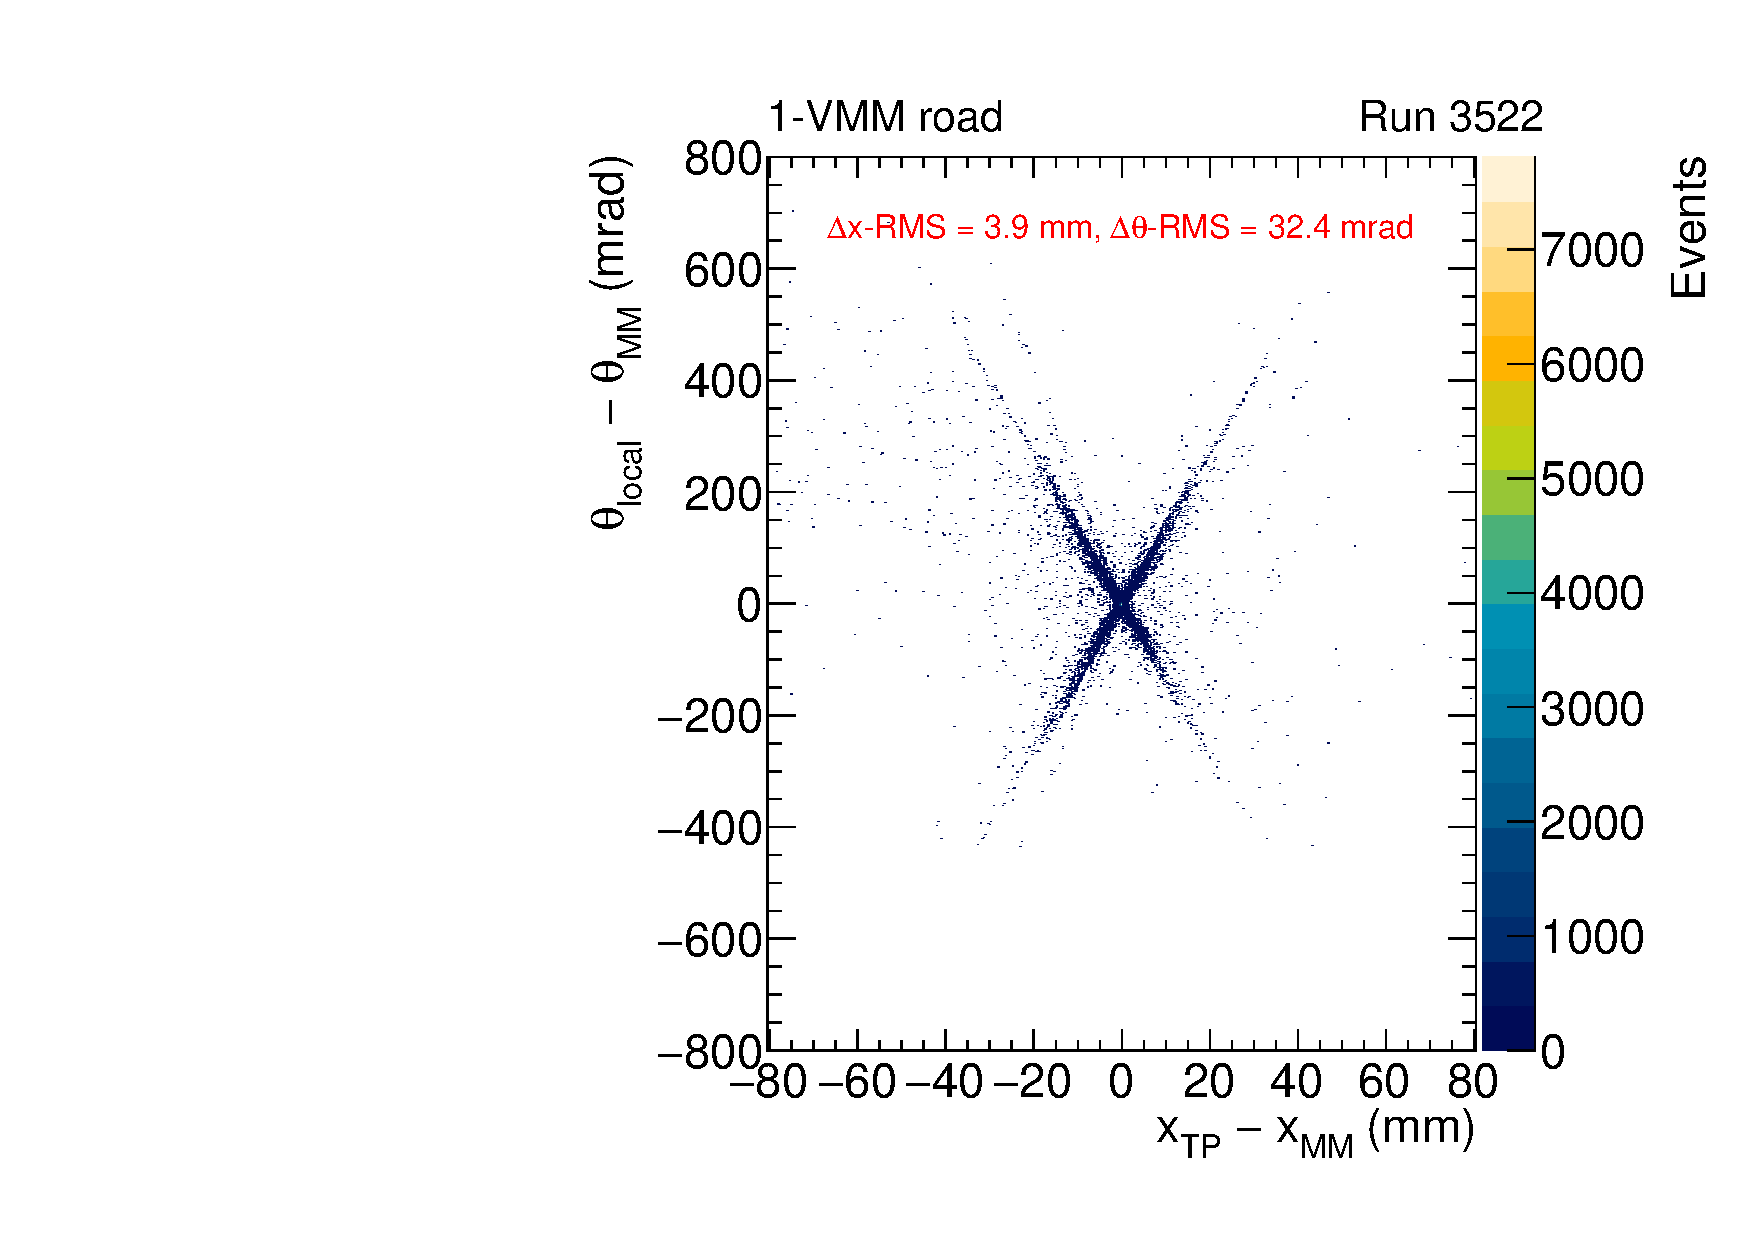
\includegraphics[width=0.48\textwidth]{figures/gbtanalysis3522/TP_xres_angres_full.pdf}
    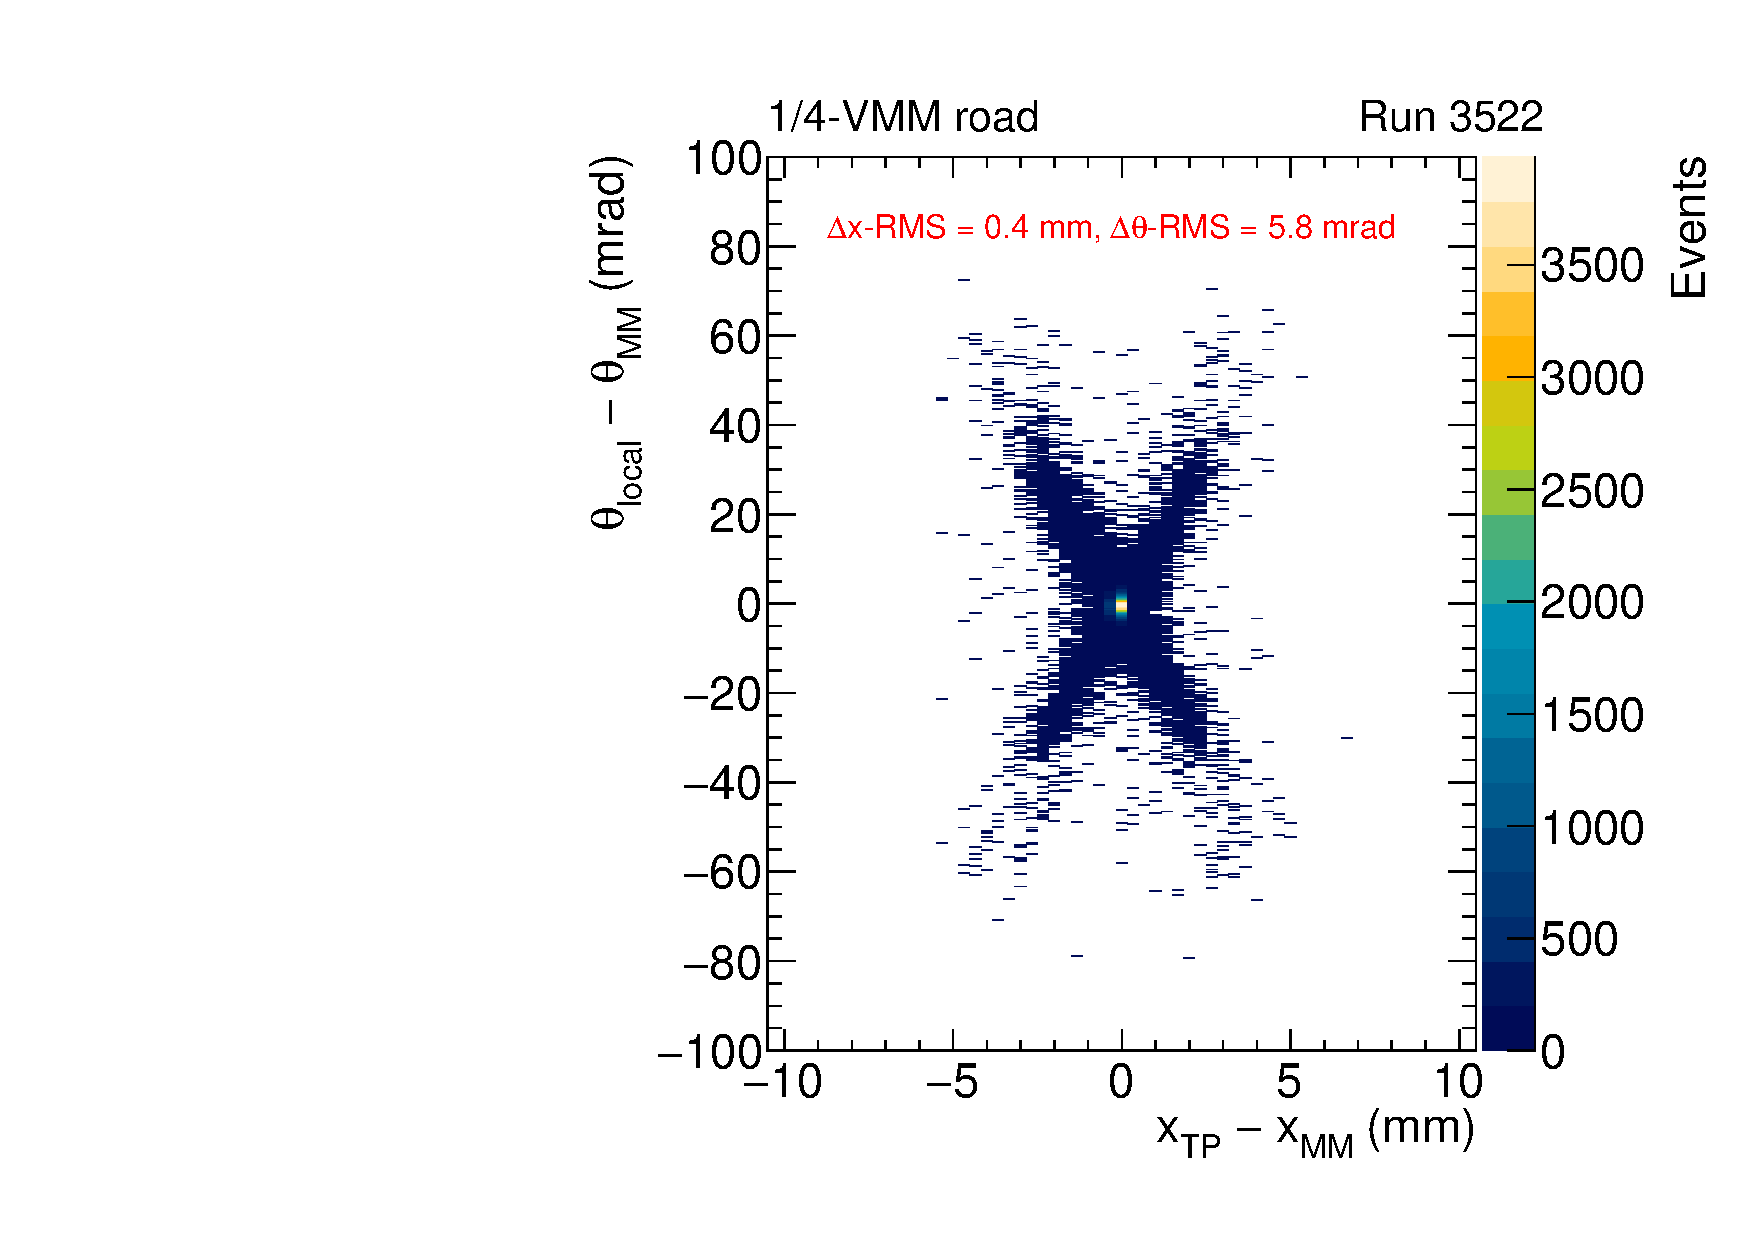
\includegraphics[width=0.48\textwidth]{figures/gbtanalysis3522/TP_xres_angres.pdf}
  \end{center}
  \vspace{-10pt}
  \caption{2D plots of $\theta_{\rm local}-\theta_{\rm MM} $ vs  $x_{\rm TP}-x_{\rm MM}$
   using 1-VMM online roads (left) and 1/4-VMM offline roads (right), 
as discussed in Section~\ref{sec:perf-roads}. The tails of the resolution are greatly suppressed with smaller roads.}
  \label{fig:xthetares}
\end{figure}
%%%%%%%%%%%%%%%%%%%%%%%%%%%%%%%%%%%%%%%%%%%%%%%%%%%%%%%%%%
\subsection{Time resolution}

 Based on a previous study of ours and prudence, the MMTP algorithm makes use of a 8 BC window to form a trigger.
  Figure~\ref{fig:time} shows the distribution of the number of BC clocks used by the algorithm to find a trigger for all events
 using a 200 ns peaktime.
  If all hits arrive at the same BC, the BC window is 1. The necessity of a larger window follows from the time jitter
  of the individual ART signals which can be better measured by the distribution of the BC difference between any two ART signal forming a trigger
  (shown also in the same figure). 
%%%%%%%%%%%%%%%%%%%%%%%%%%%%%%
\begin{figure}[!htpb]
  \begin{center}
    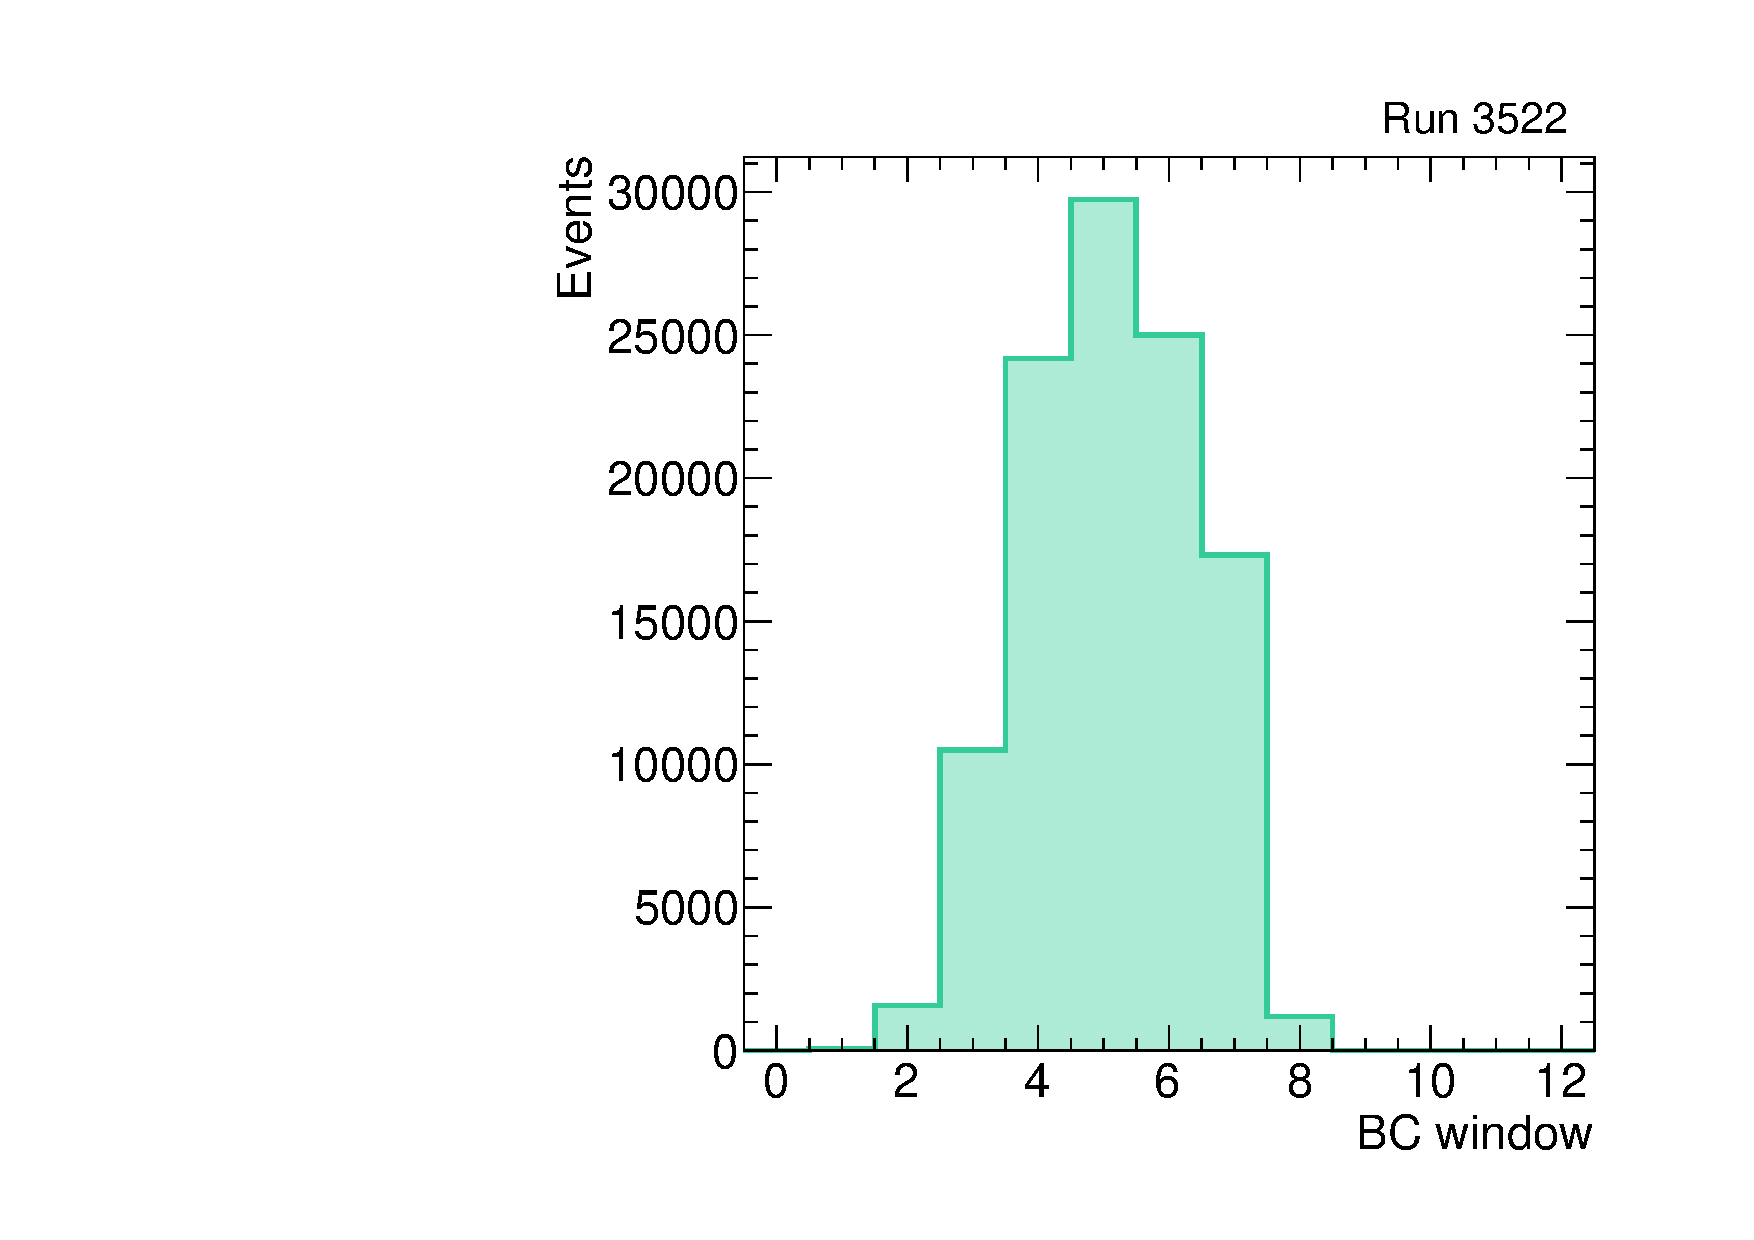
\includegraphics[width=0.48\textwidth]{figures/gbtanalysis3522/artwin_lin.pdf}
    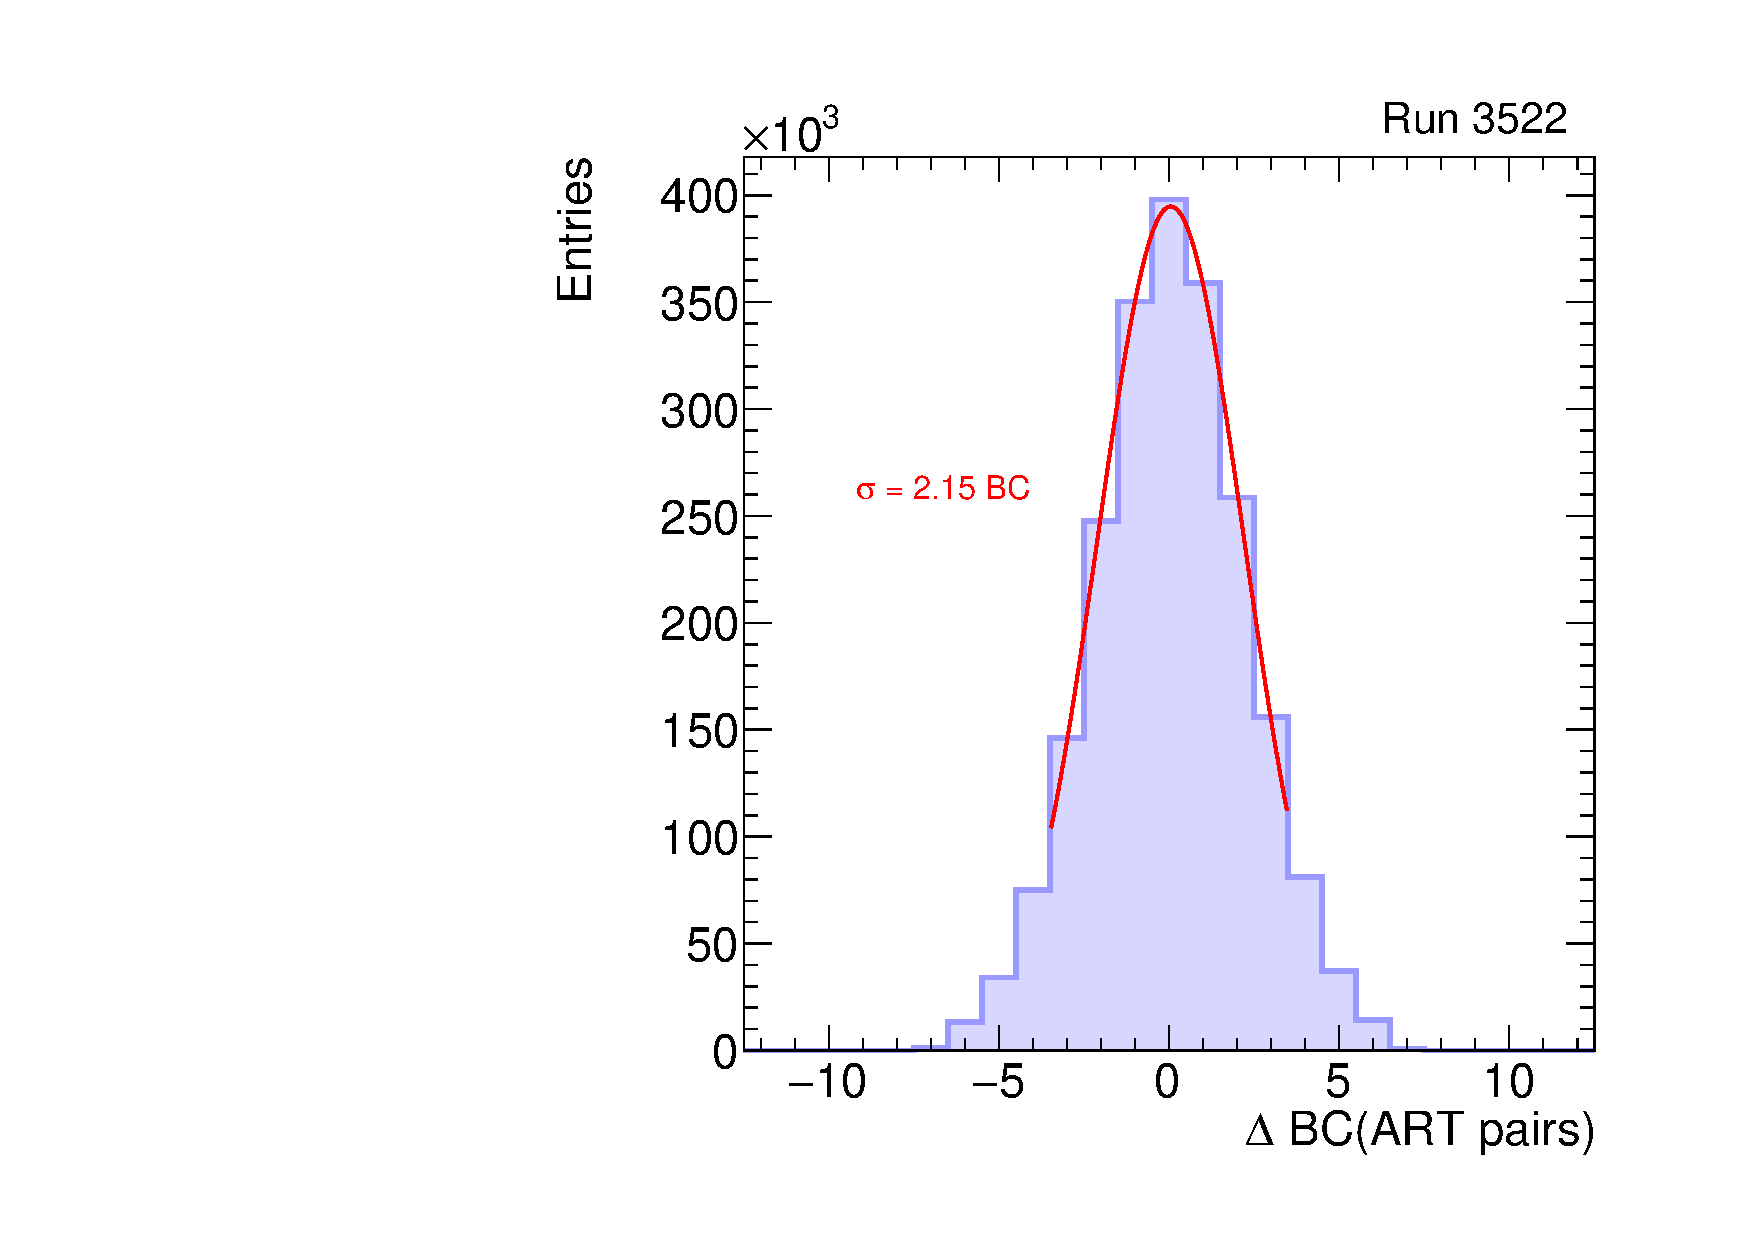
\includegraphics[width=0.48\textwidth]{figures/gbtanalysis3522/artrpairs_lin.pdf}
  \end{center}
  \vspace{-10pt}
  \caption{Distribution of the BC window used to produced a trigger for all events (left); Distribution of the BC difference of all pairs of ART signals
 forming a trigger (right). The data are  well described by a Gaussian function. The $\sigma$ written in the plot is the result of the fit to this
 distribution.}
  \label{fig:time}
\end{figure}
%%%%%%%%%%%%%%%%%%%%%%%%%%%%%%%%%%%%%
The time distribution of ART signals is fairly well described by a Gaussian function
 with a $\sigma$ of 40 ns.


The  precise measurement of the trigger BCID  is needed to match tracks found in the NSW with tracks found by the TGCs in
 the big wheel.
 We use two methods to define the trigger BCID: the average of the BCID of all hits and the BCID of the earliest hit.
 As shown in  Fig.~\ref{fig:timeres}, the resolution is approxinmately 1 BC.
%%%%%%%%%%%%%%%%%%%%%%%%%%%%%%%%%%%%
\begin{figure}[!htpb]
  \begin{center}
    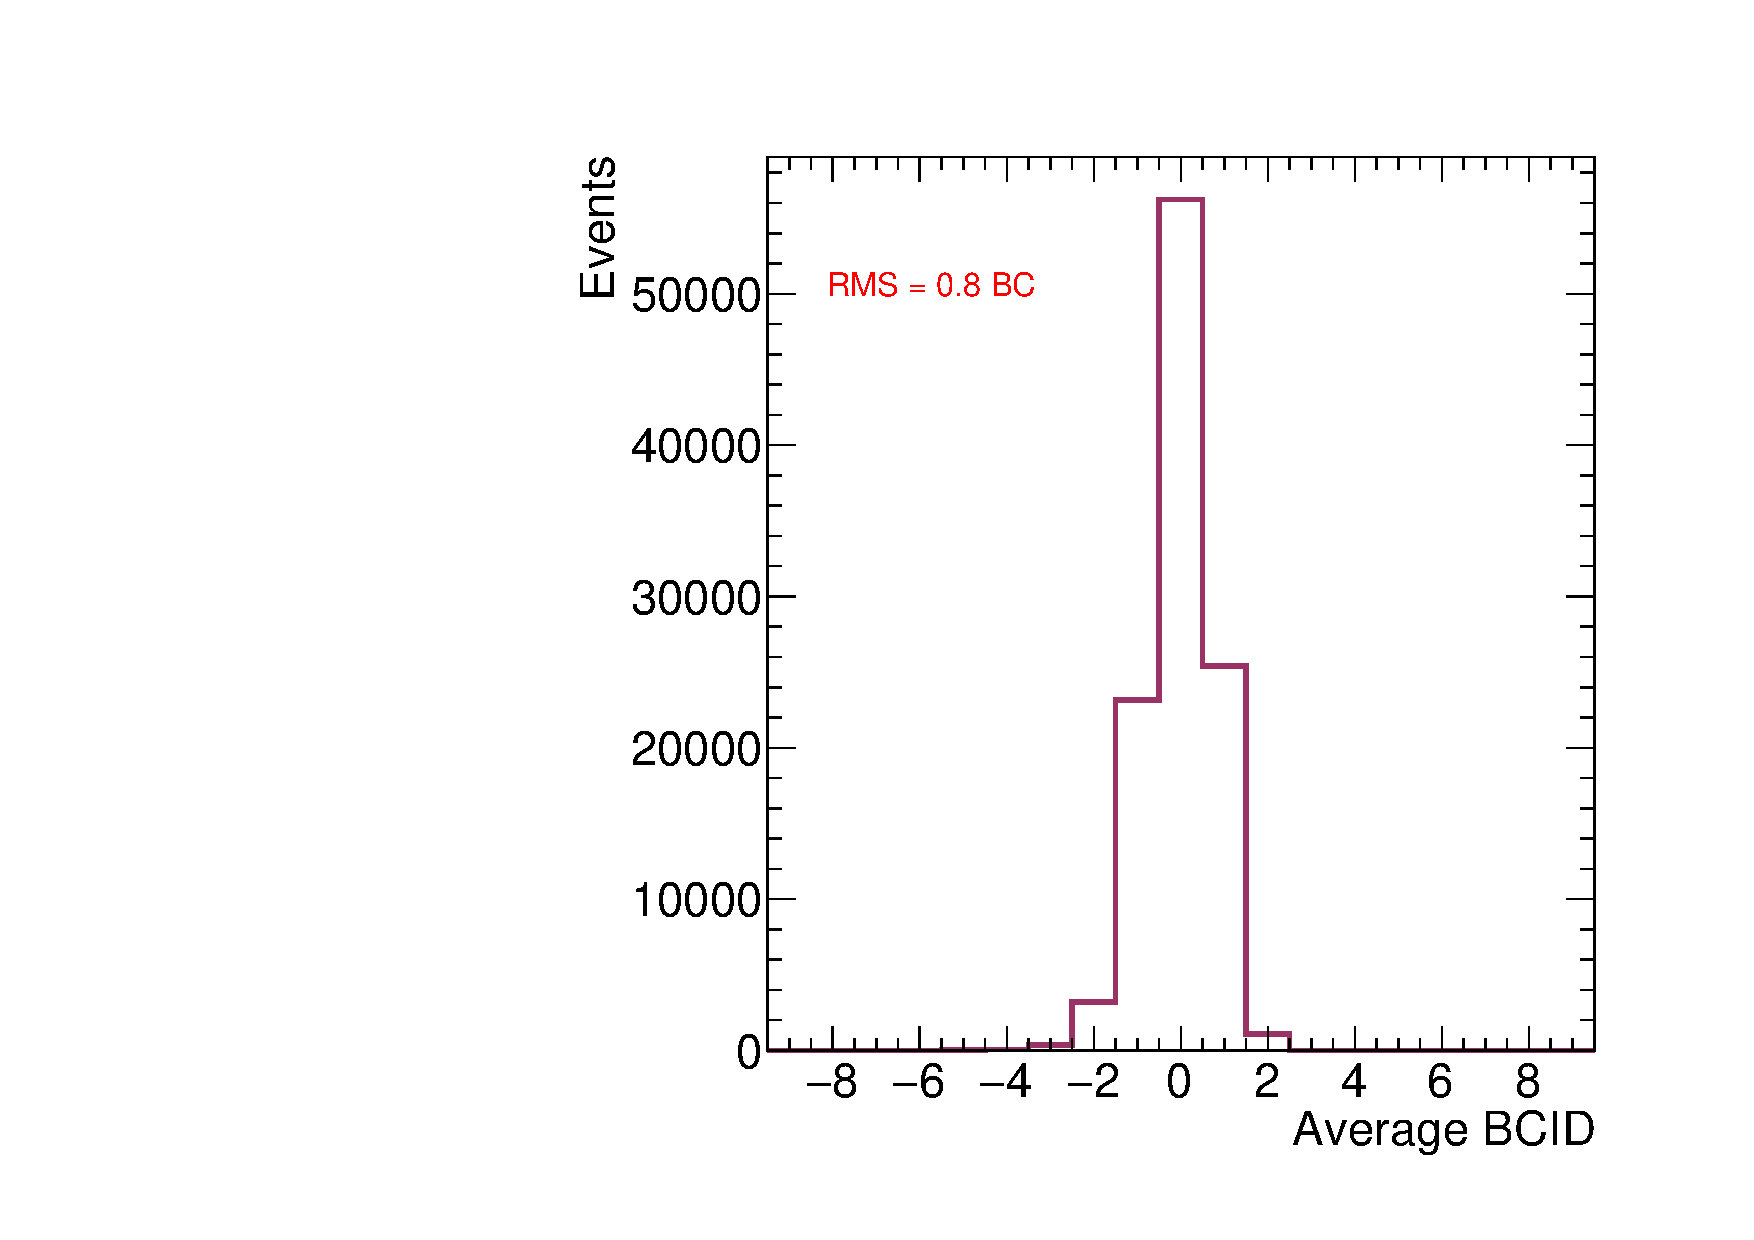
\includegraphics[width=0.48\textwidth]{figures/gbtanalysis3522/avg_BCID.pdf}
    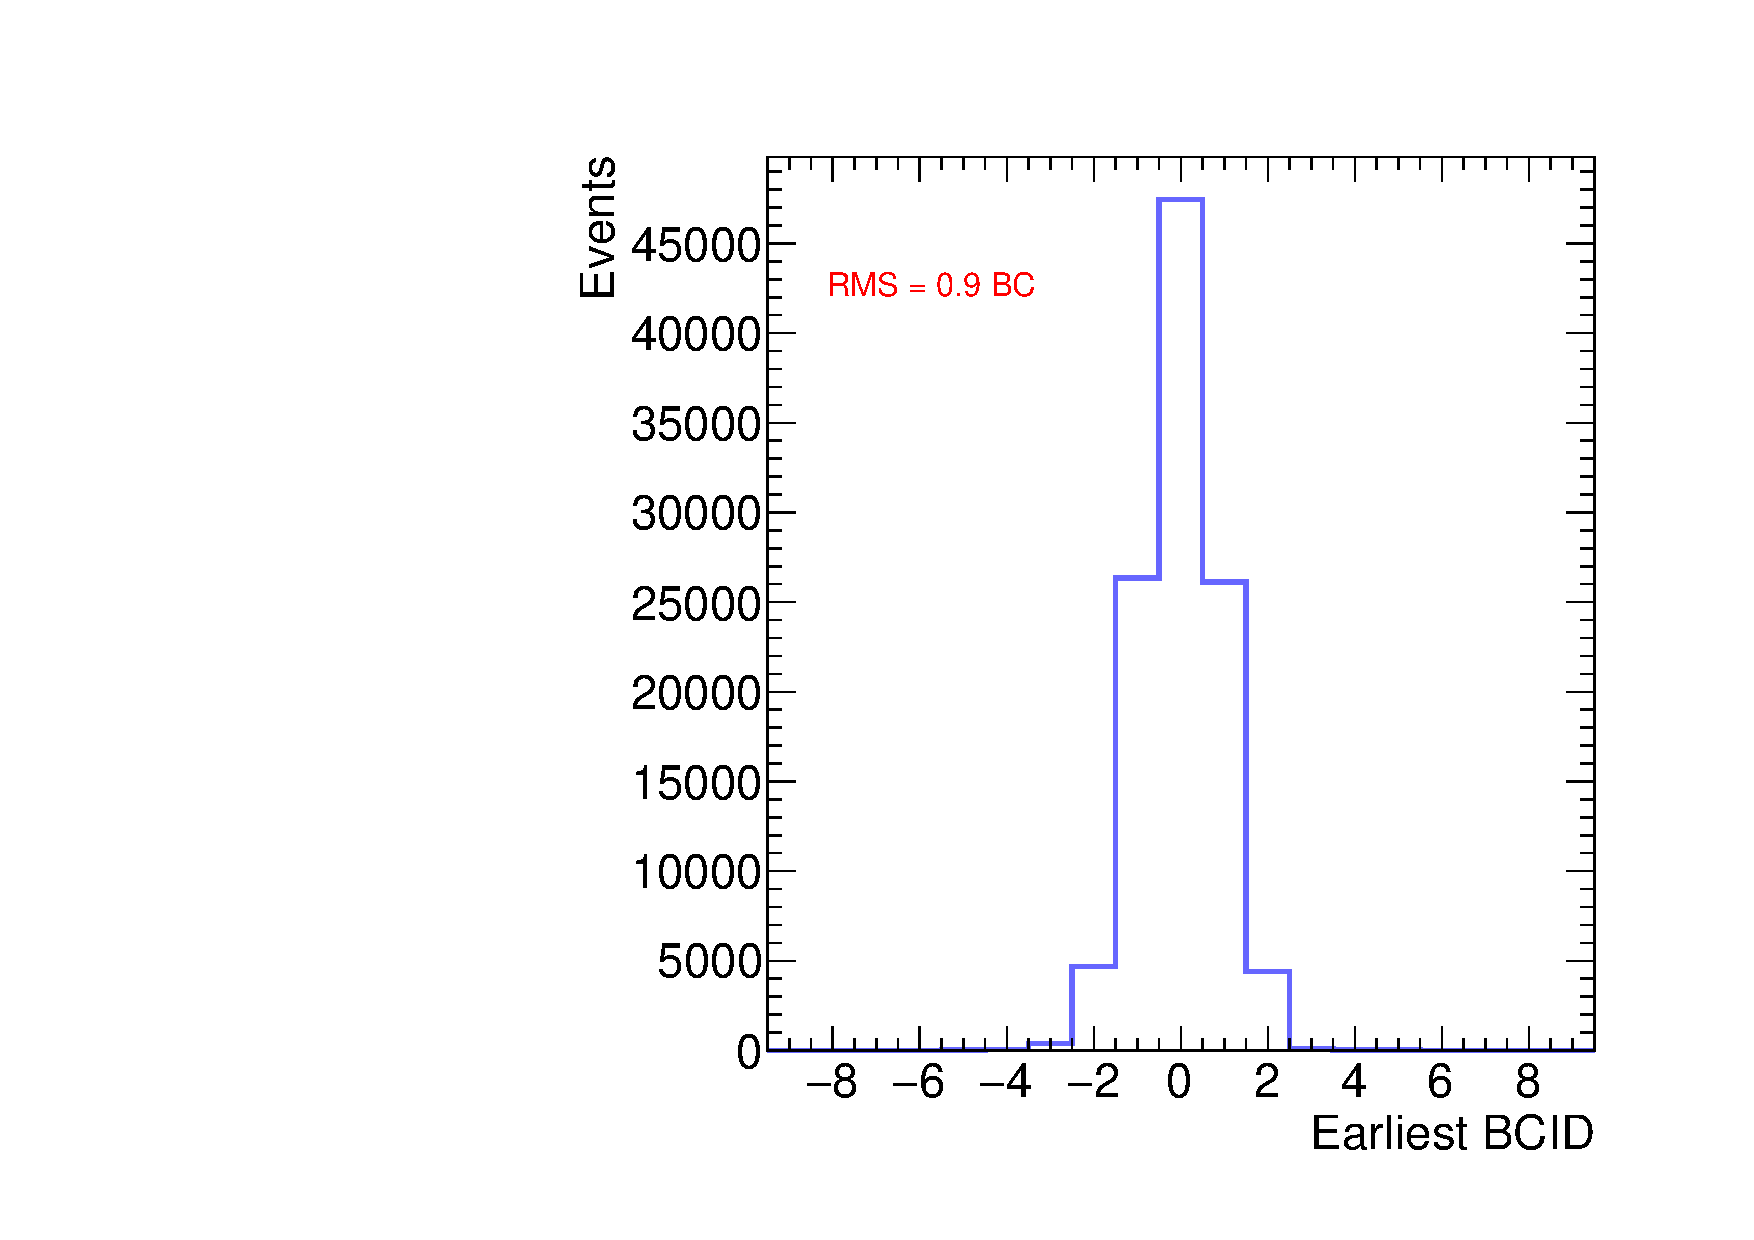
\includegraphics[width=0.48\textwidth]{figures/gbtanalysis3522/earliest_BCID.pdf}
  \end{center}
  \vspace{-10pt}
  \caption{Distributions of the BCID difference between the scintillator trigger and the MMTP trigger.
  The scintillator trigger has a time resolution of 0.05 BCID.}          
  \label{fig:timeres}
\end{figure}
%%%%%%%%%%%%%%%%%%%%%%%%%%%%%%%%%%%%%%%
\subsection{Peaktime dependence}
\label{sec:perf-integ}
It is a urban legend that the time-jitter of the ART signal generated at threshold is dominated by the variation of the signal
amplitude. In Ref.~\cite{oldart}, we did show that the time jitter is mildly affected by this cause.
In the following, we check this again using  200 ns, 100 ns, and 50 ns peaktimes.

We run our detector at very high voltage and gain. The detector efficiency is little affected by the chosen peaktime. The cluster multiplicity
decreases by $\simeq$ 5\% when halving the peaktime.

 The time distributions, analogous to those in Fig.~\ref{fig:time} to~\ref{fig:timeres}
 are shown in Fig.~\ref{fig:integ_window} to~\ref{fig:integ_avg_earliest}. 
 The time distribution of individual ART follows is Gaussian function with $\sigma$ decreasing from 40 ns to 32 ns when reducing the peaktime from 200 ns to 50 ns.
%%%%%%%%%%%%%%%%%%%%%%%%%%%%%%%%%%%%%%
\begin{figure}[!htpb]
  \begin{center}
    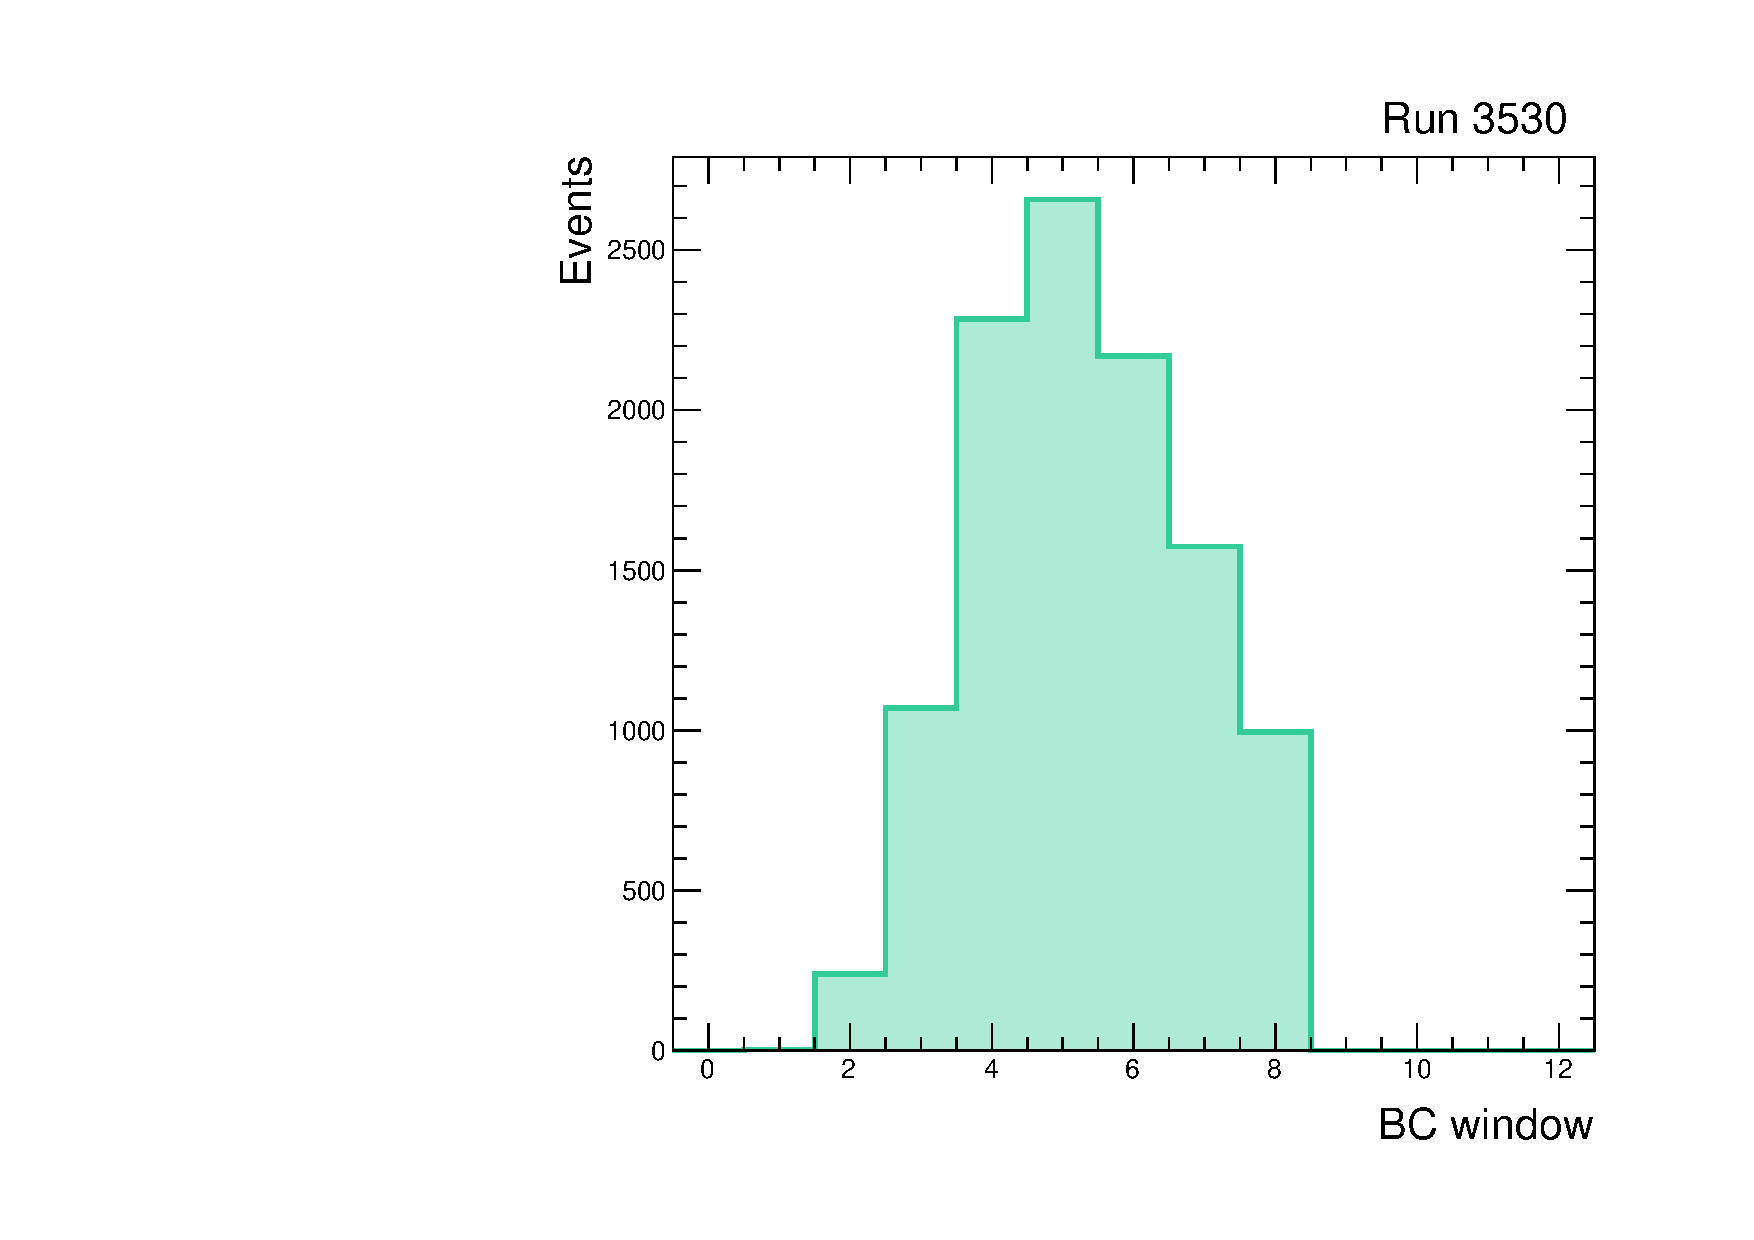
\includegraphics[width=0.3\textwidth]{figures/gbtanalysis3530/artwin_lin.pdf}
    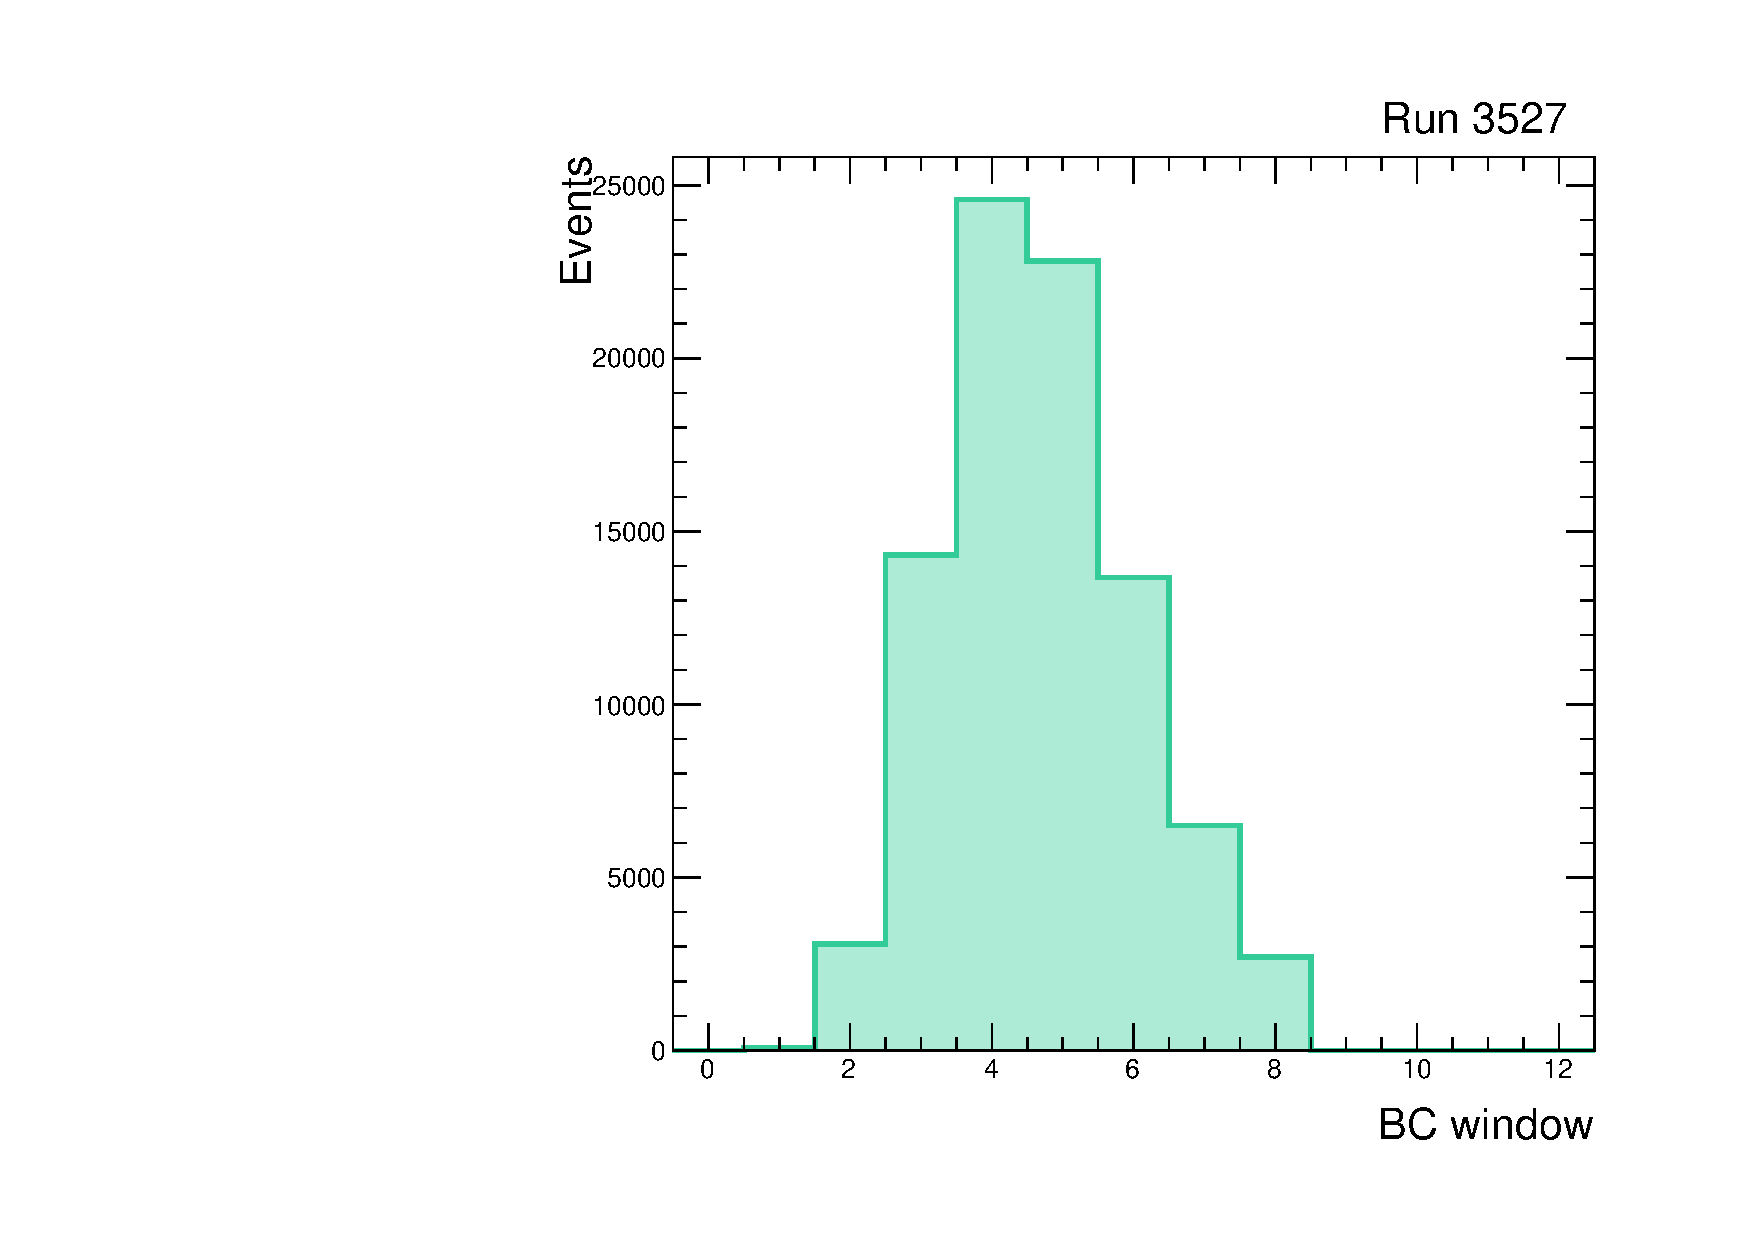
\includegraphics[width=0.3\textwidth]{figures/gbtanalysis3527/artwin_lin.pdf}
    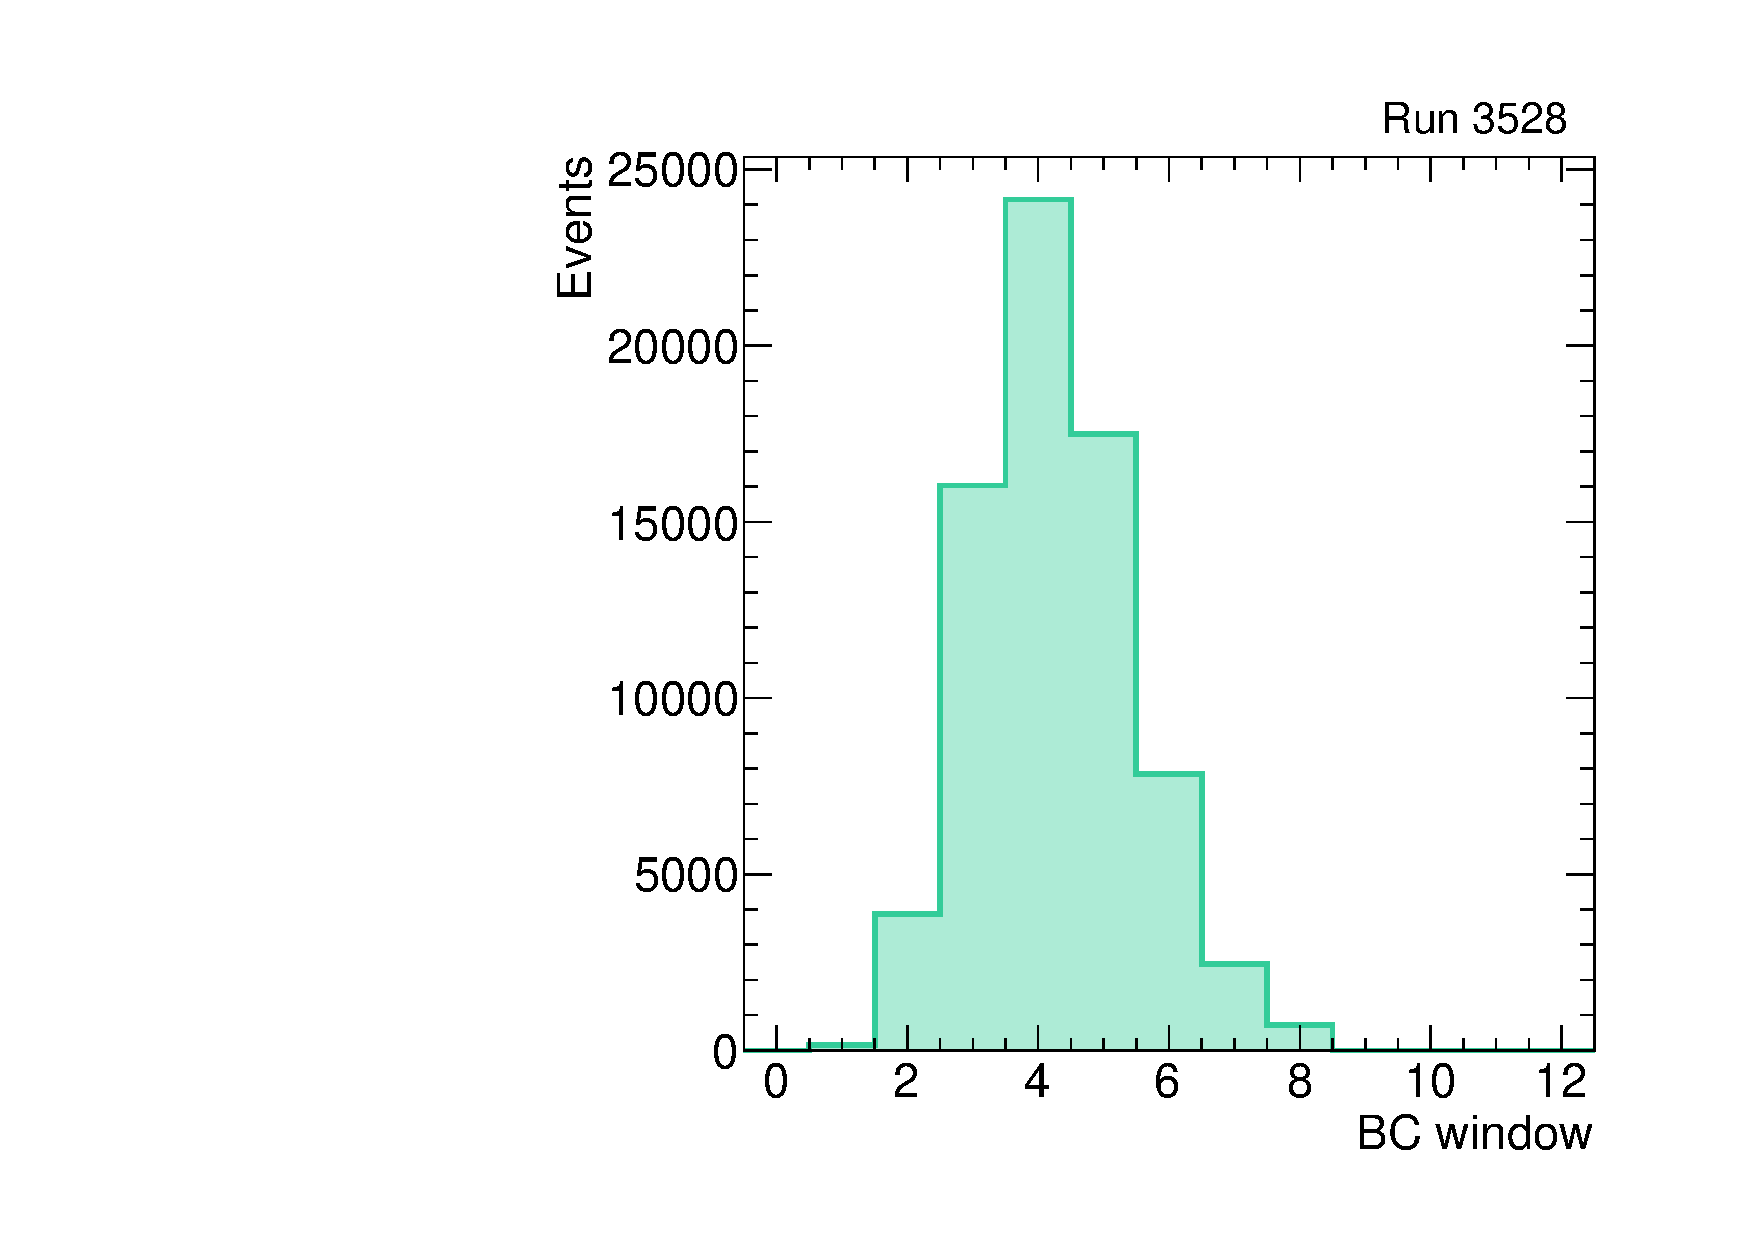
\includegraphics[width=0.3\textwidth]{figures/gbtanalysis3528/artwin_lin.pdf}
  \end{center}
  \vspace{-10pt}
  \caption{Distribution of the BC window used to produced a trigger for all events collected with (left) 200, (center) 100, and  (right) 50 ns peaktime.}
  \label{fig:integ_window}
\end{figure}
%%%%%%%%%%%%%%%%%%%%%%%%%%%%%%%%%%%%%%%%%%%%%%%%%%%%%%%%%%
\begin{figure}[!htpb]
  \begin{center}
    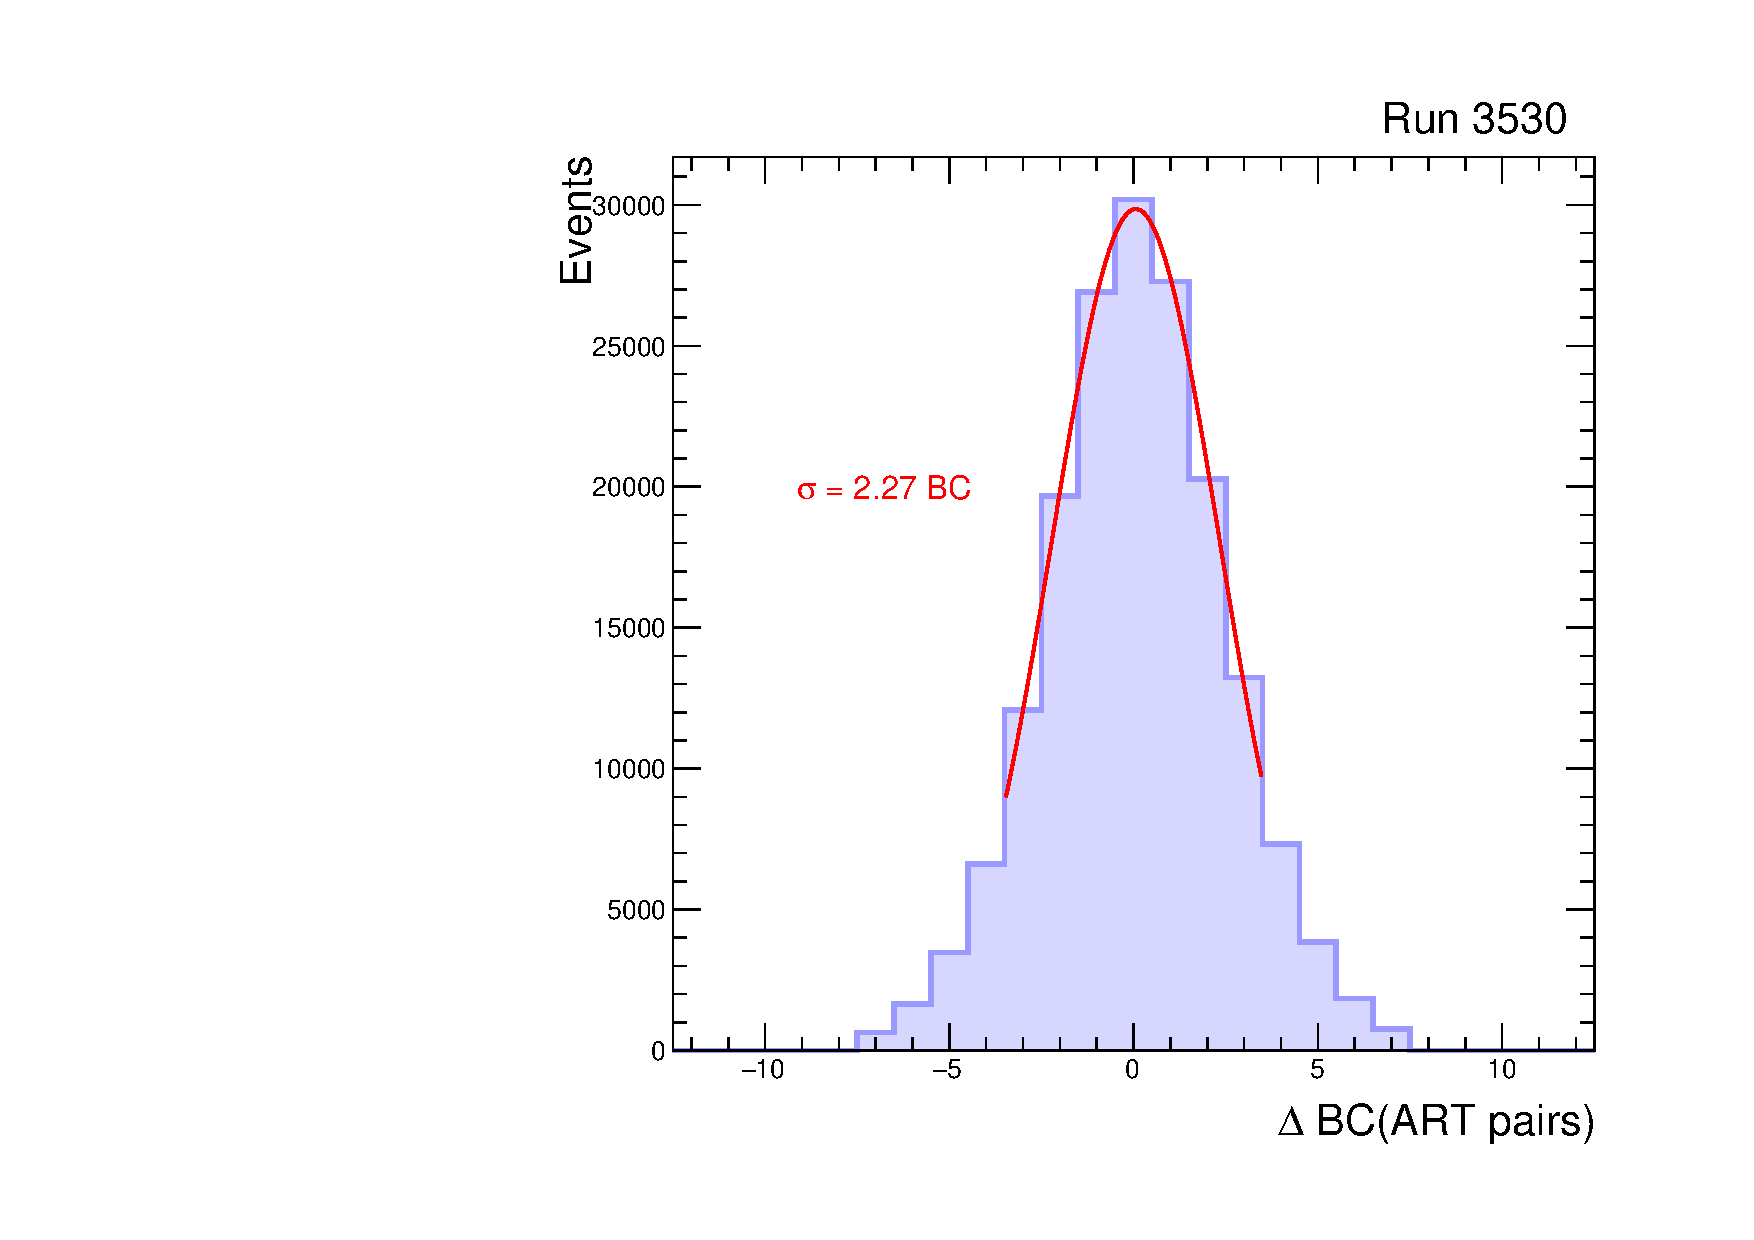
\includegraphics[width=0.3\textwidth]{figures/gbtanalysis3530/artrpairs_lin.pdf}
    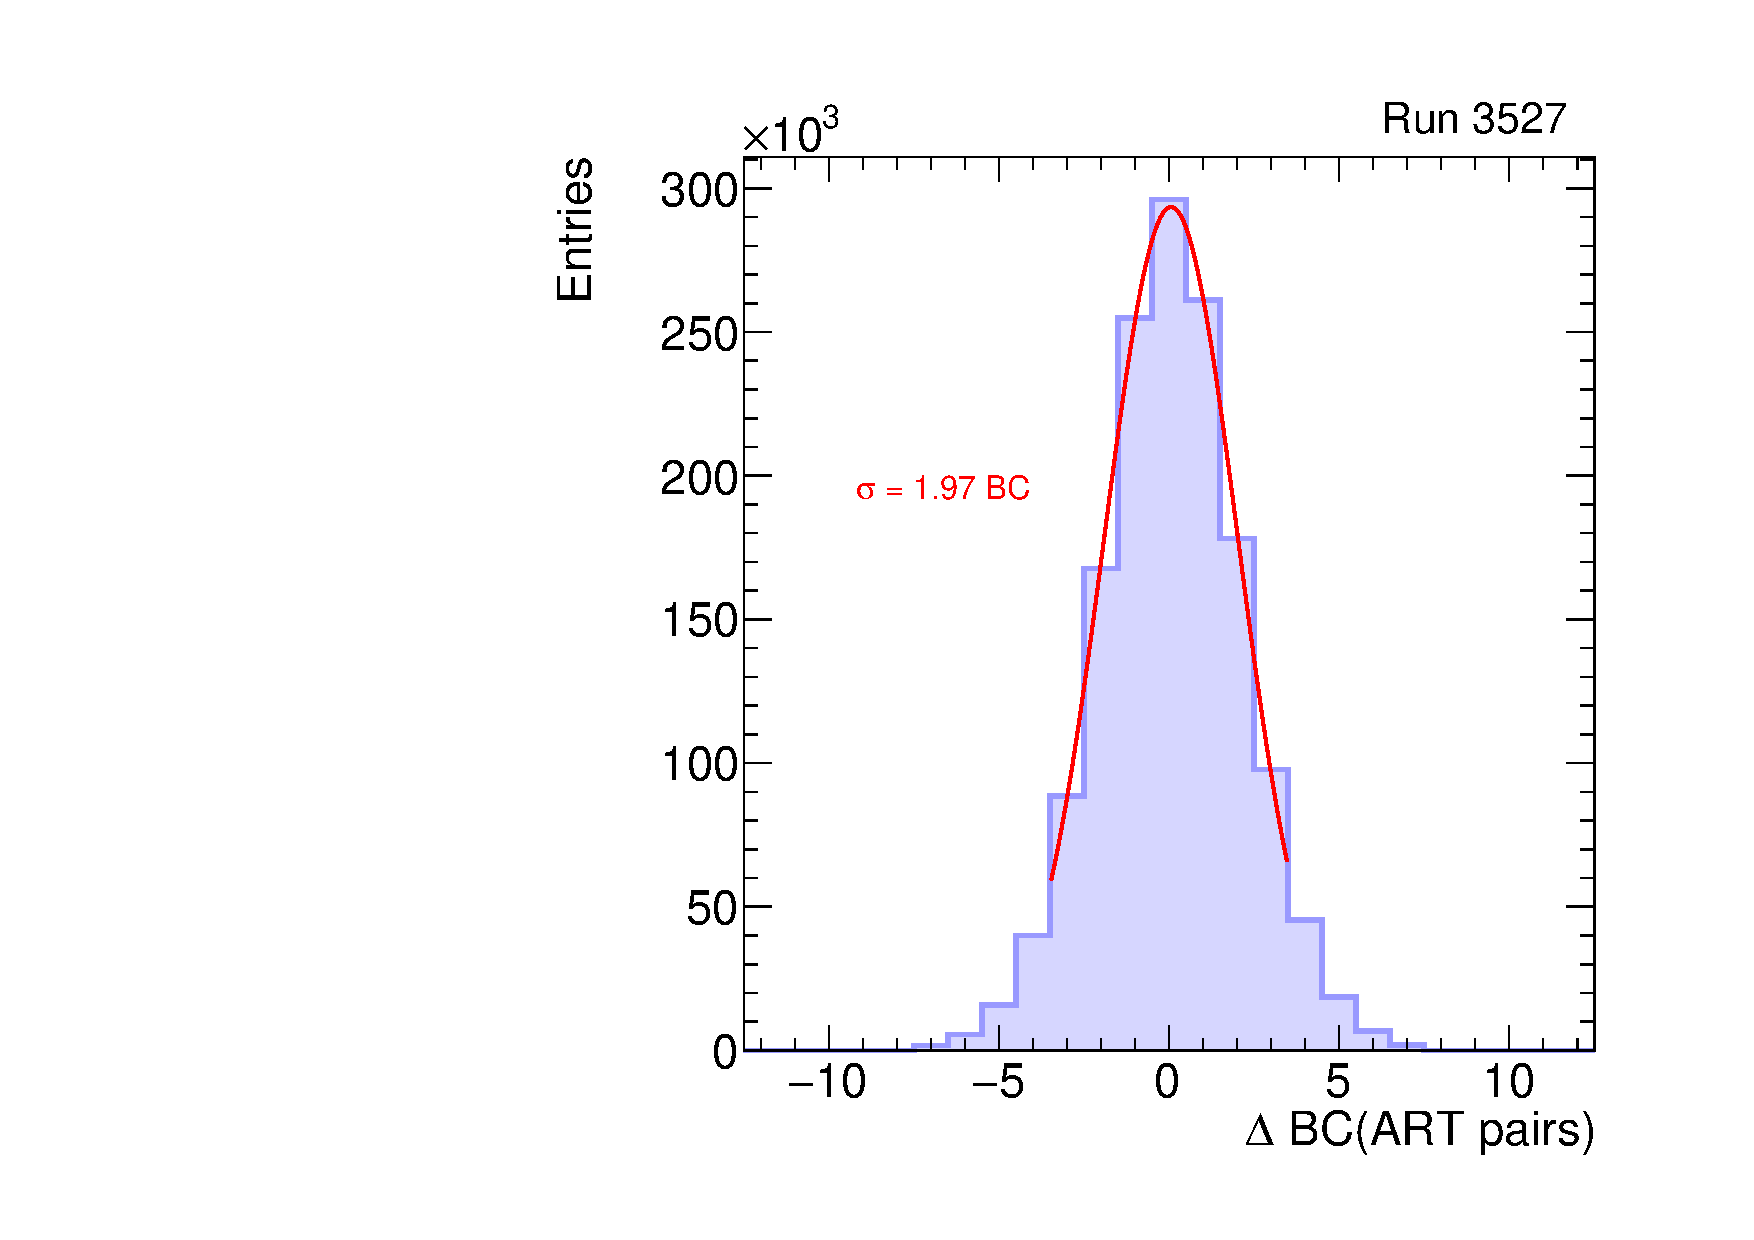
\includegraphics[width=0.3\textwidth]{figures/gbtanalysis3527/artrpairs_lin.pdf}
    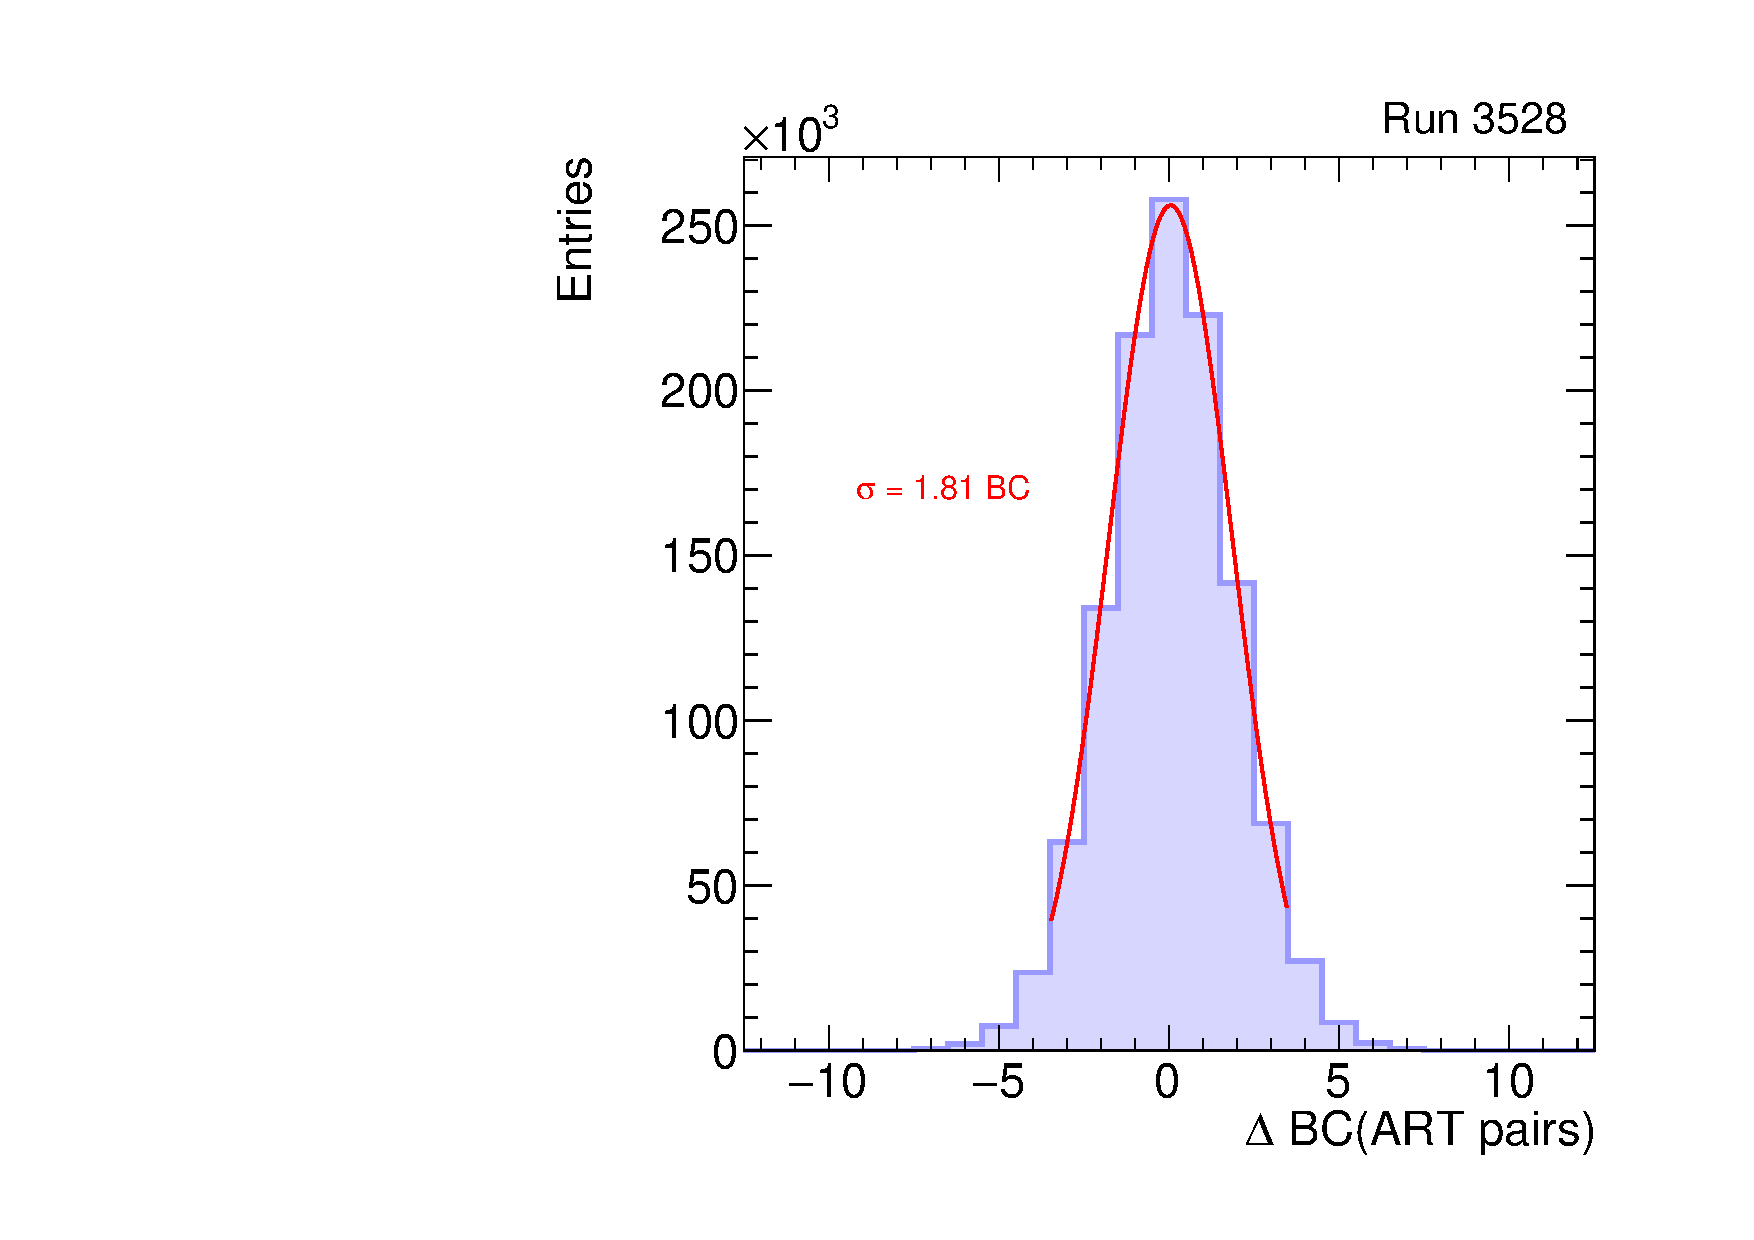
\includegraphics[width=0.3\textwidth]{figures/gbtanalysis3528/artrpairs_lin.pdf}
  \end{center}
  \vspace{-10pt}
  \caption{ Distribution of the BC difference of all pairs of ART signals
 forming a trigger  for all events collected with (left) 200, (center) 100, and  (right) 50 ns peaktime.
 The data are  well described by a Gaussian function. The $\sigma$ written in the plot is the result of the fit to this
 distribution.}
  \label{fig:integ_pairs}
\end{figure}
%%%%%%%%%%%%%%%%%%%%%%%%%%%%%%%%%%%%%%%%%%%%%%%%%%%%%%%%%%%%%
\begin{figure}[!htpb]
  \begin{center}
    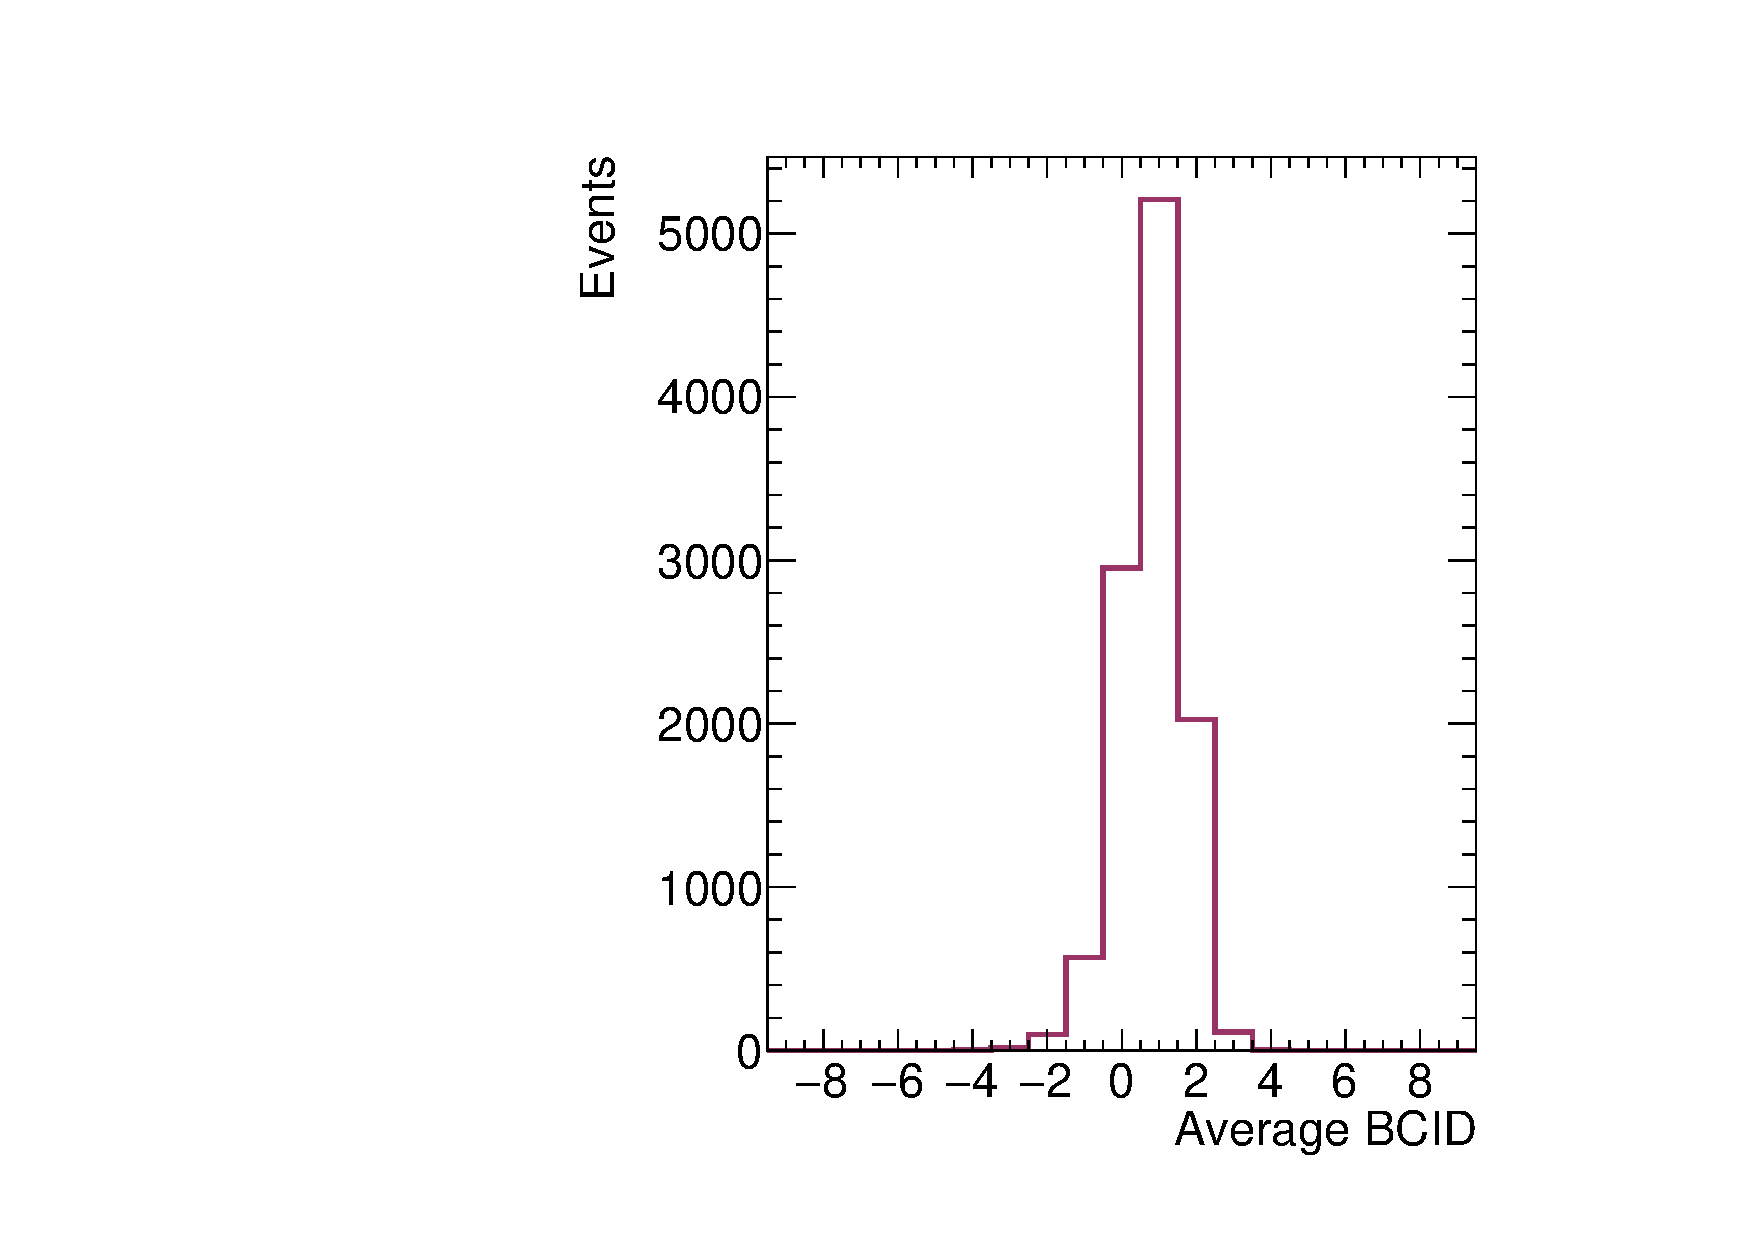
\includegraphics[width=0.3\textwidth]{figures/gbtanalysis3530/avg_BCID.pdf}
    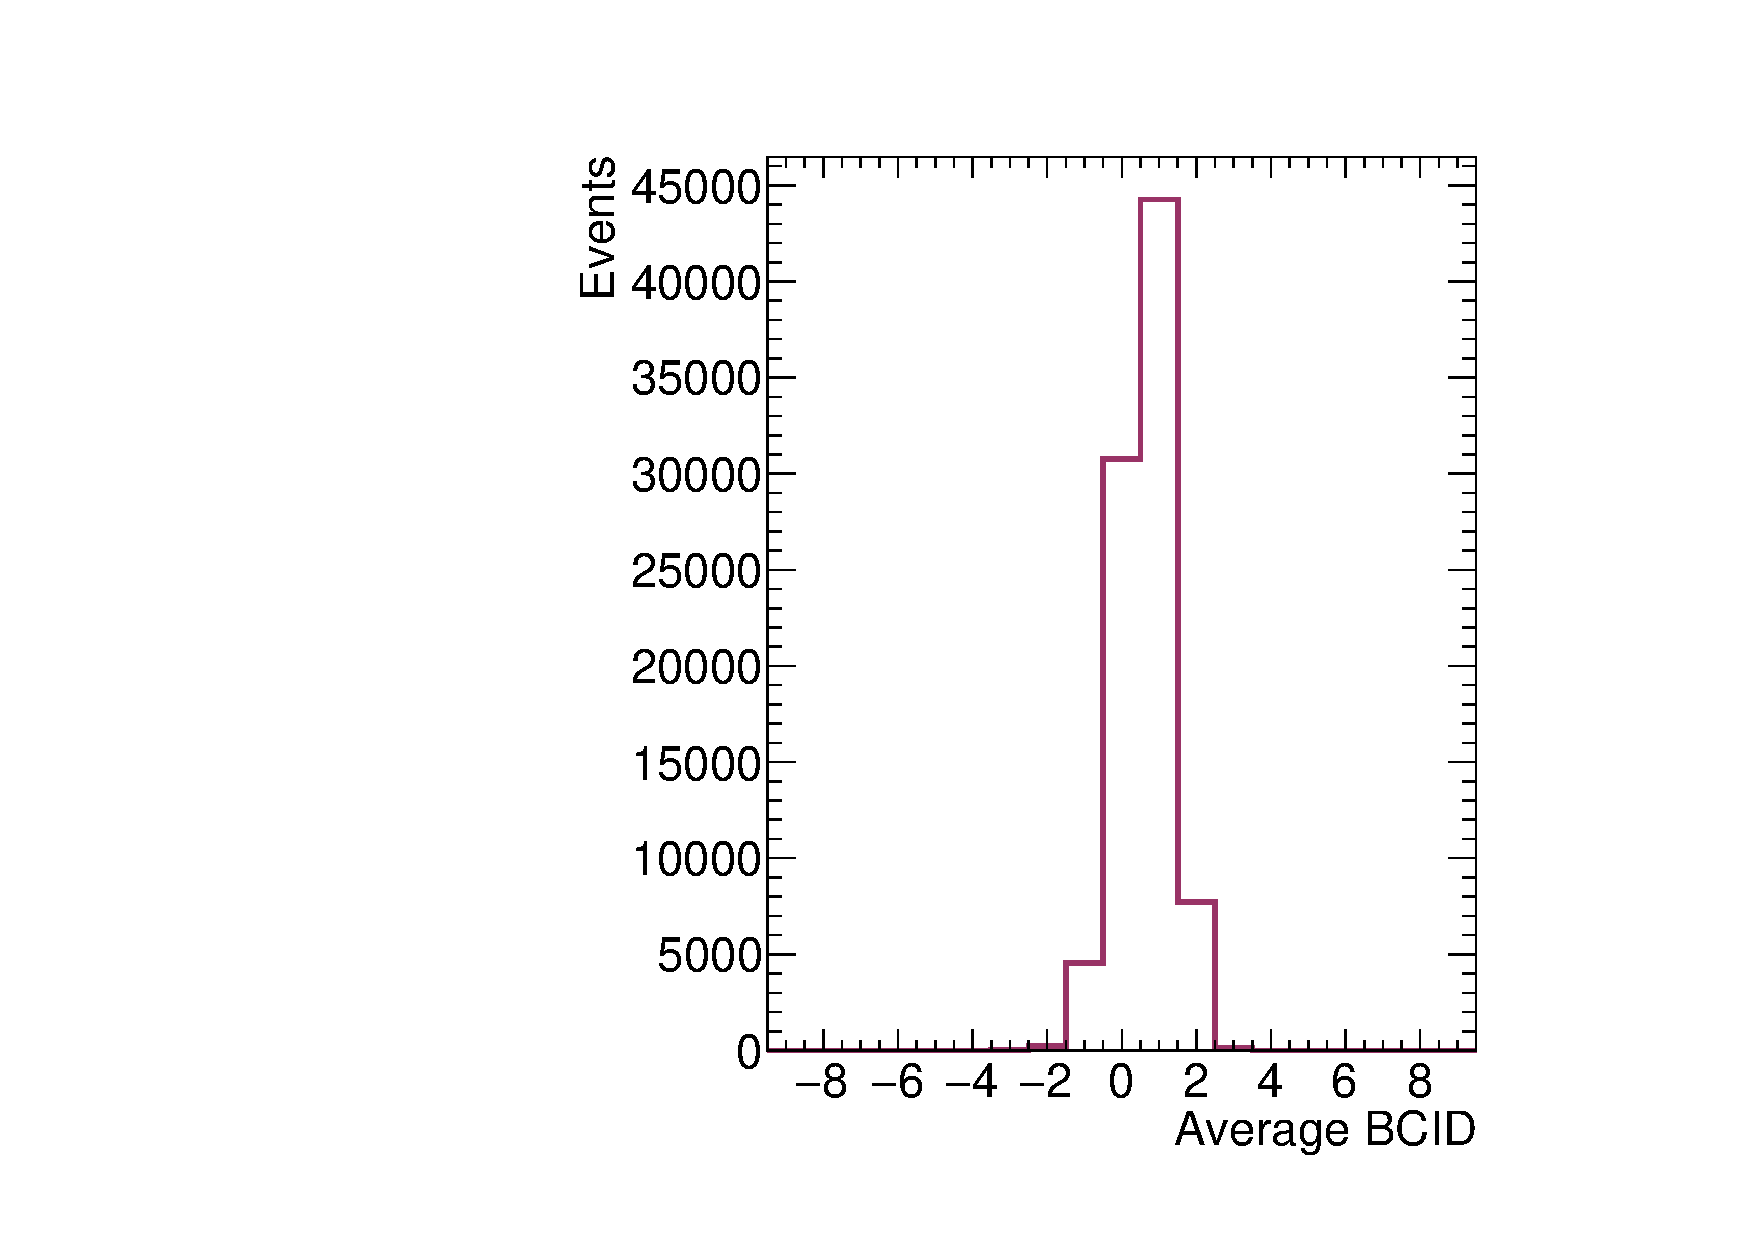
\includegraphics[width=0.3\textwidth]{figures/gbtanalysis3527/avg_BCID.pdf}
    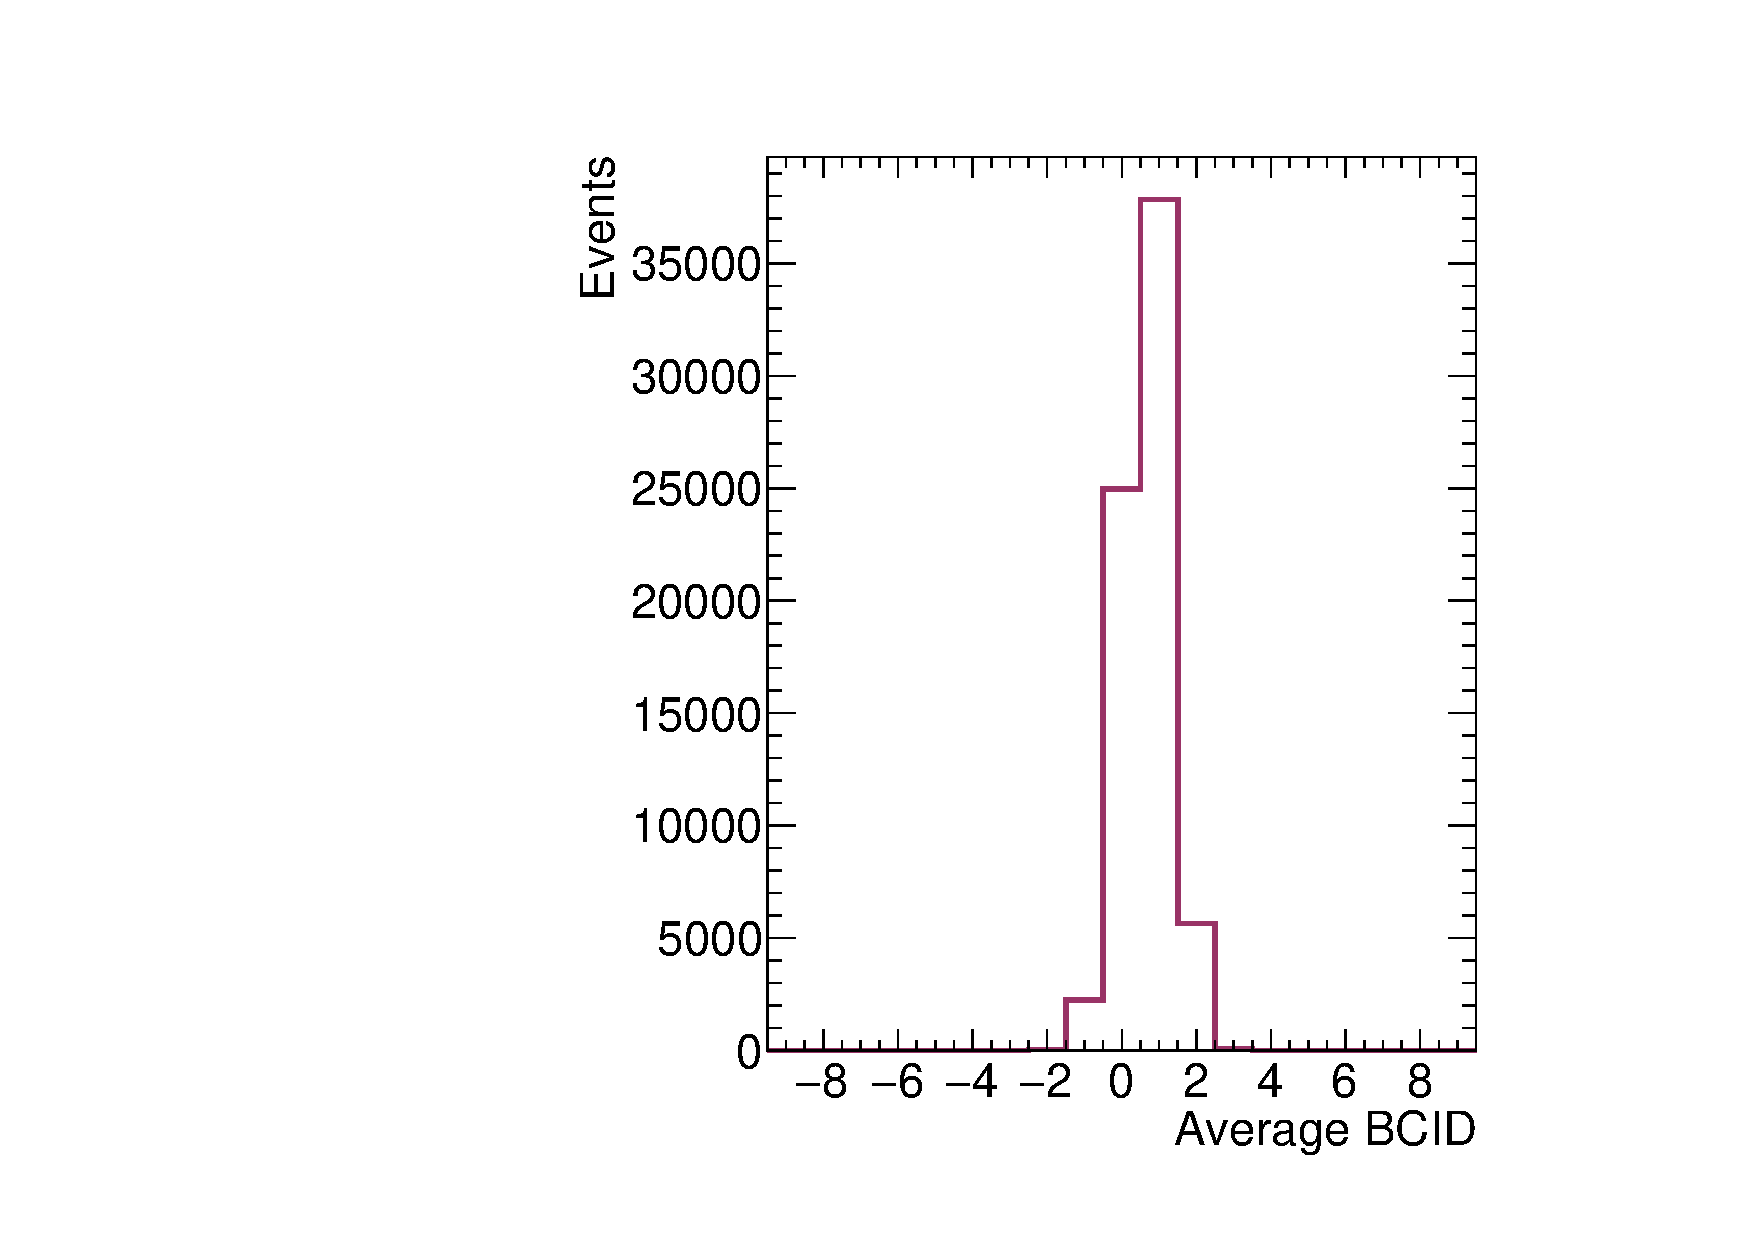
\includegraphics[width=0.3\textwidth]{figures/gbtanalysis3528/avg_BCID.pdf}
  \end{center}
  \vspace{-10pt}
  \caption{Distributions of the BCID difference between the scintillator trigger and the MMTP trigger
 for all events collected with (left) 200, (center) 100, and  (right) 50 ns peaktime.
 The MMTP  time is evaluated as as the average BCID of the ART hits.}
  \label{fig:integ_avg_bc}
\end{figure}
%%%%%%%%%%%%%%%%%%%%%%%%%%%%%%%%%%%%%%%%%%%%%%%%%%%%%%%%%%
\begin{figure}[!htpb]
  \begin{center}
    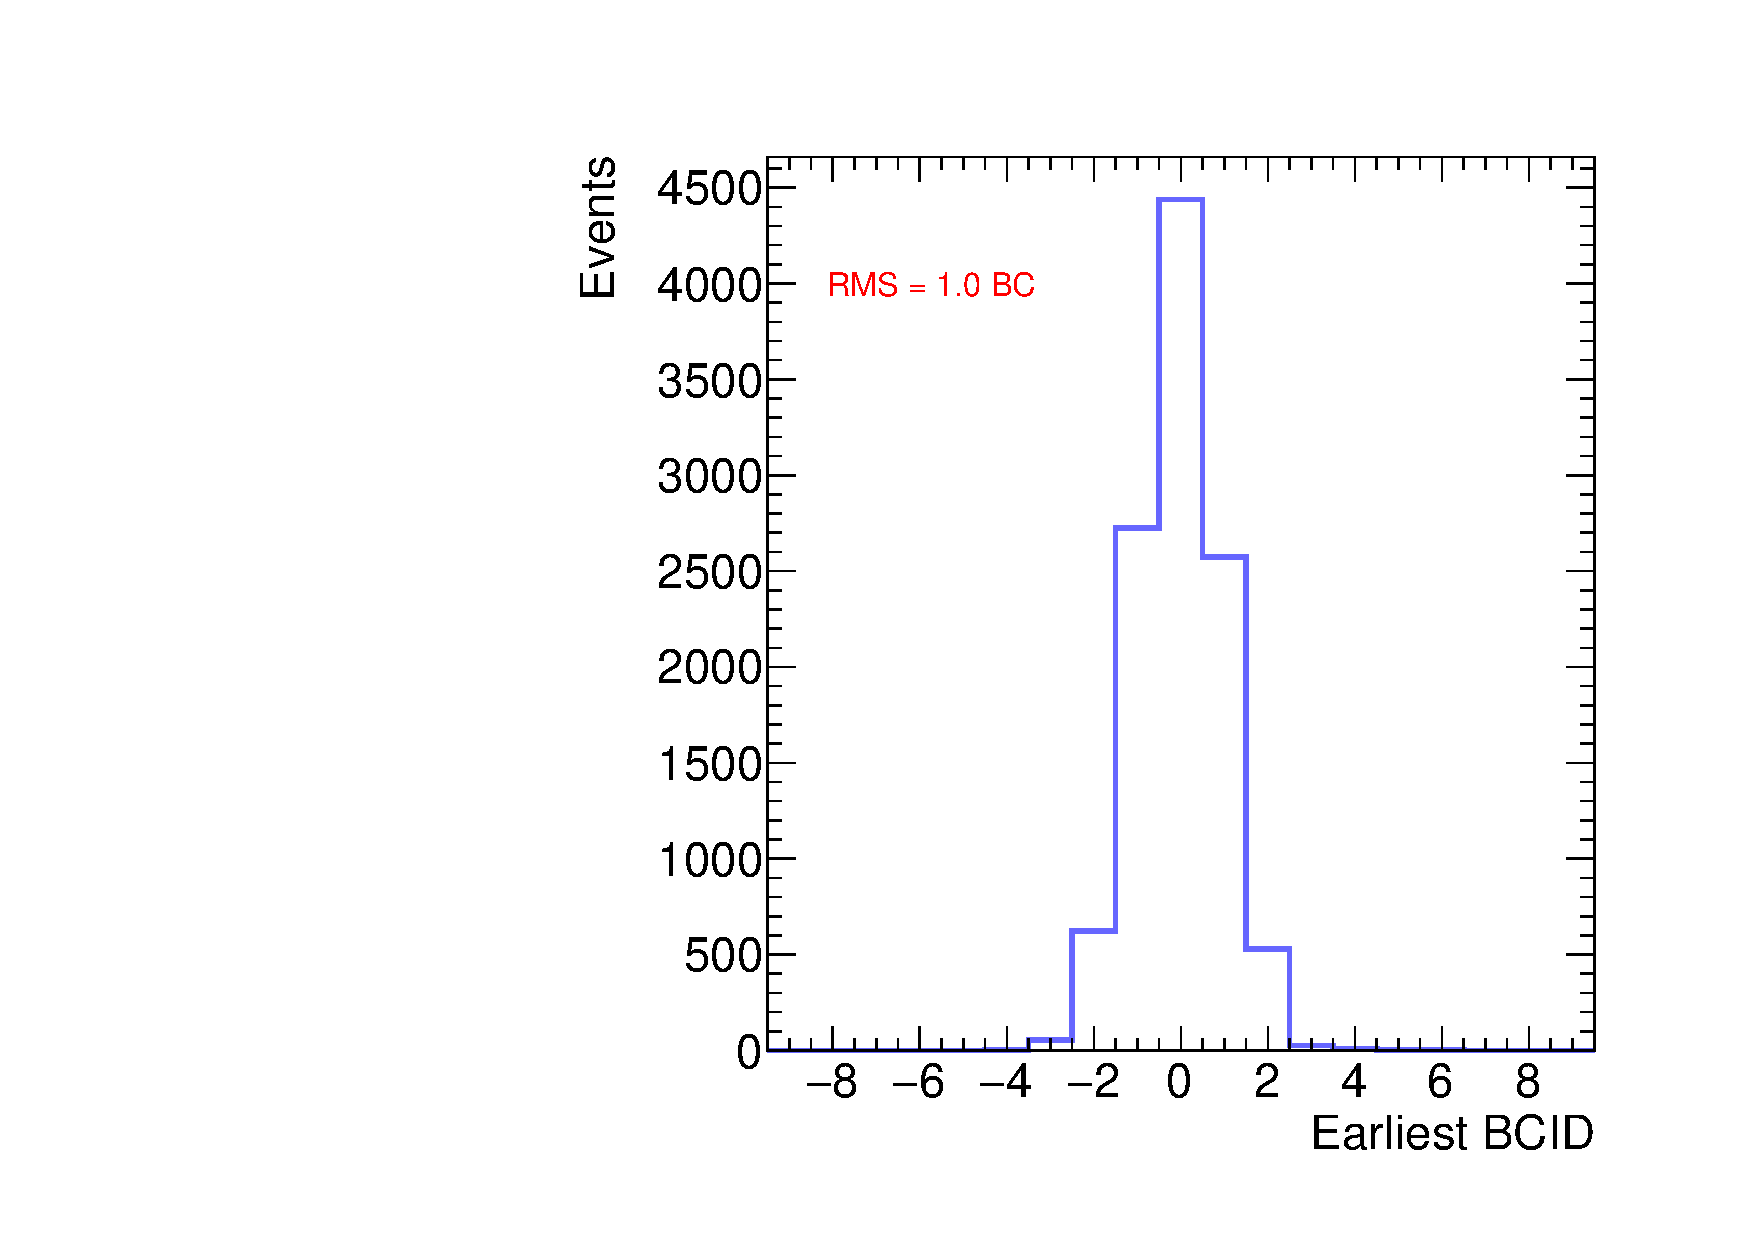
\includegraphics[width=0.3\textwidth]{figures/gbtanalysis3530/earliest_BCID.pdf}
    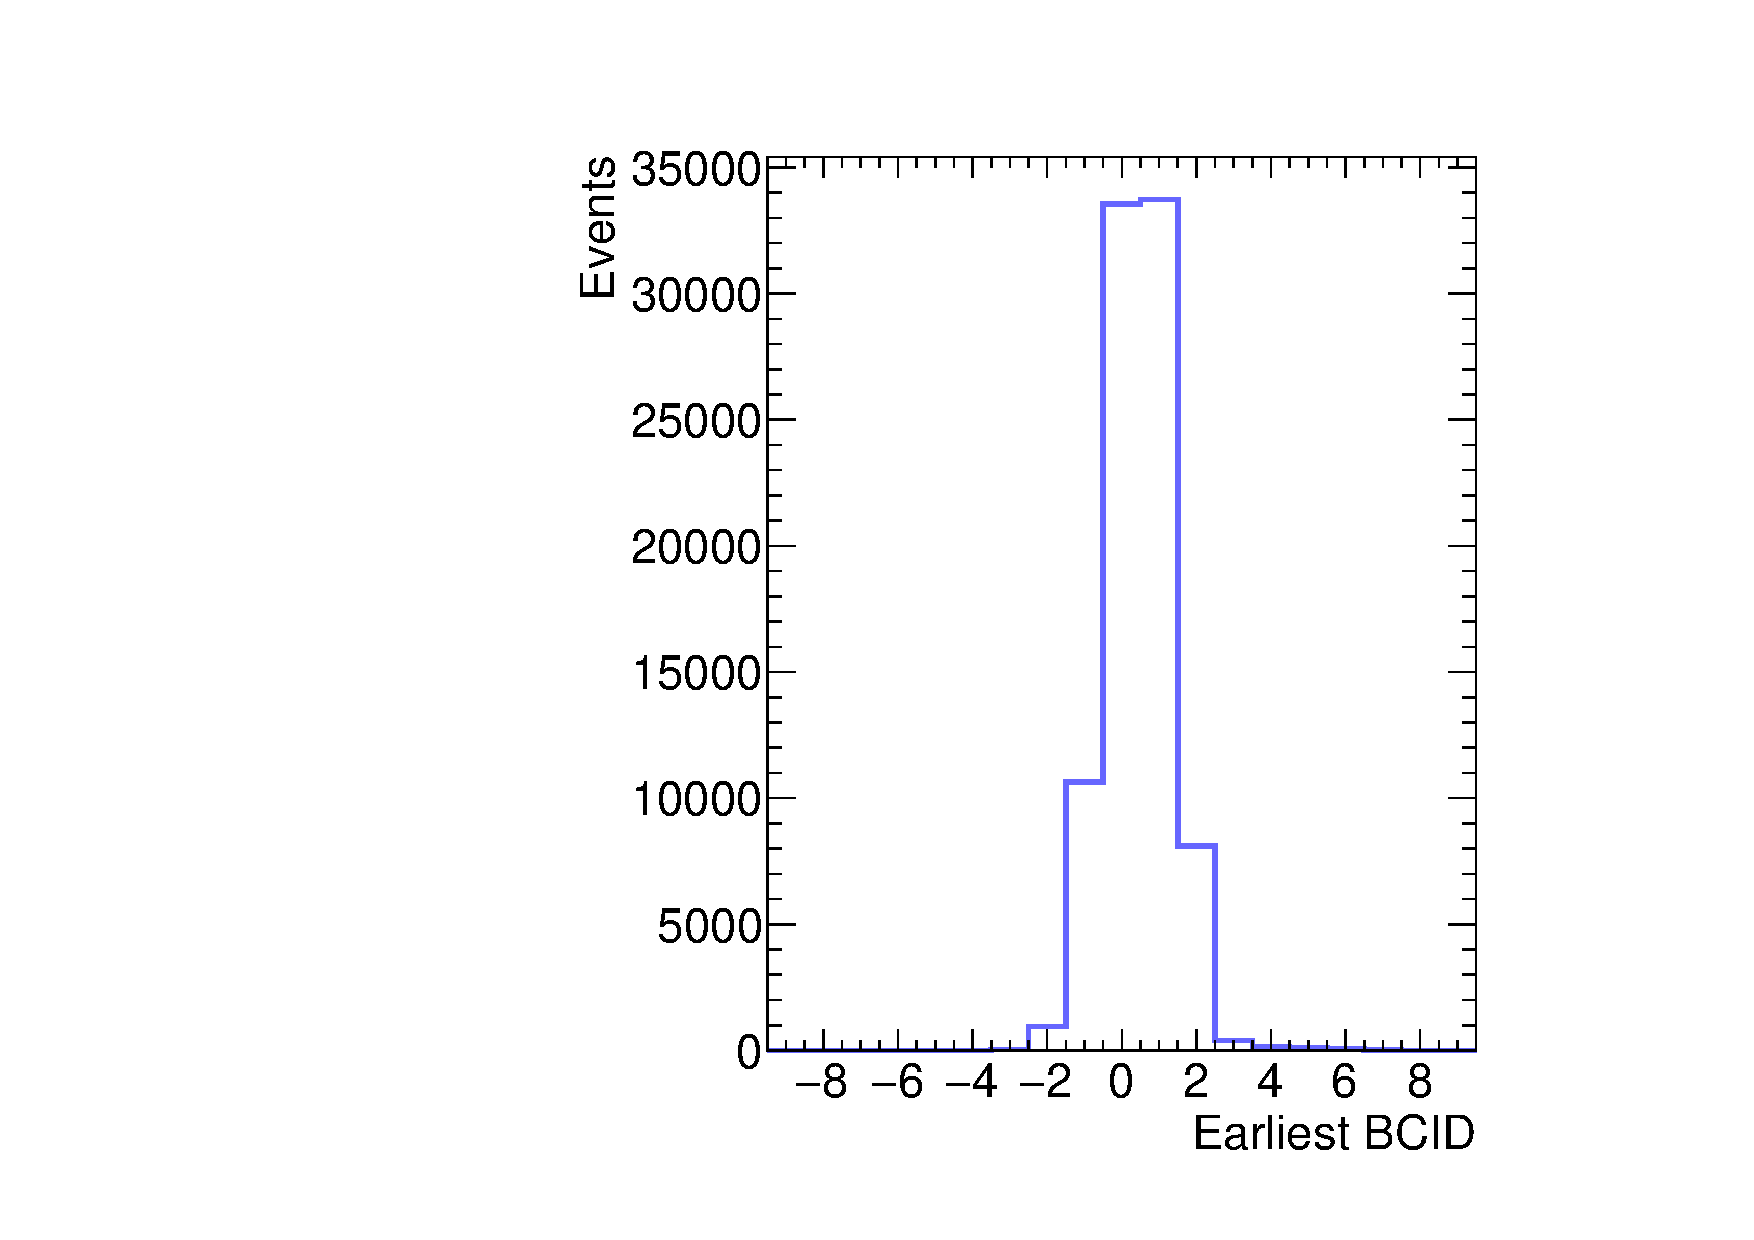
\includegraphics[width=0.3\textwidth]{figures/gbtanalysis3527/earliest_BCID.pdf}
    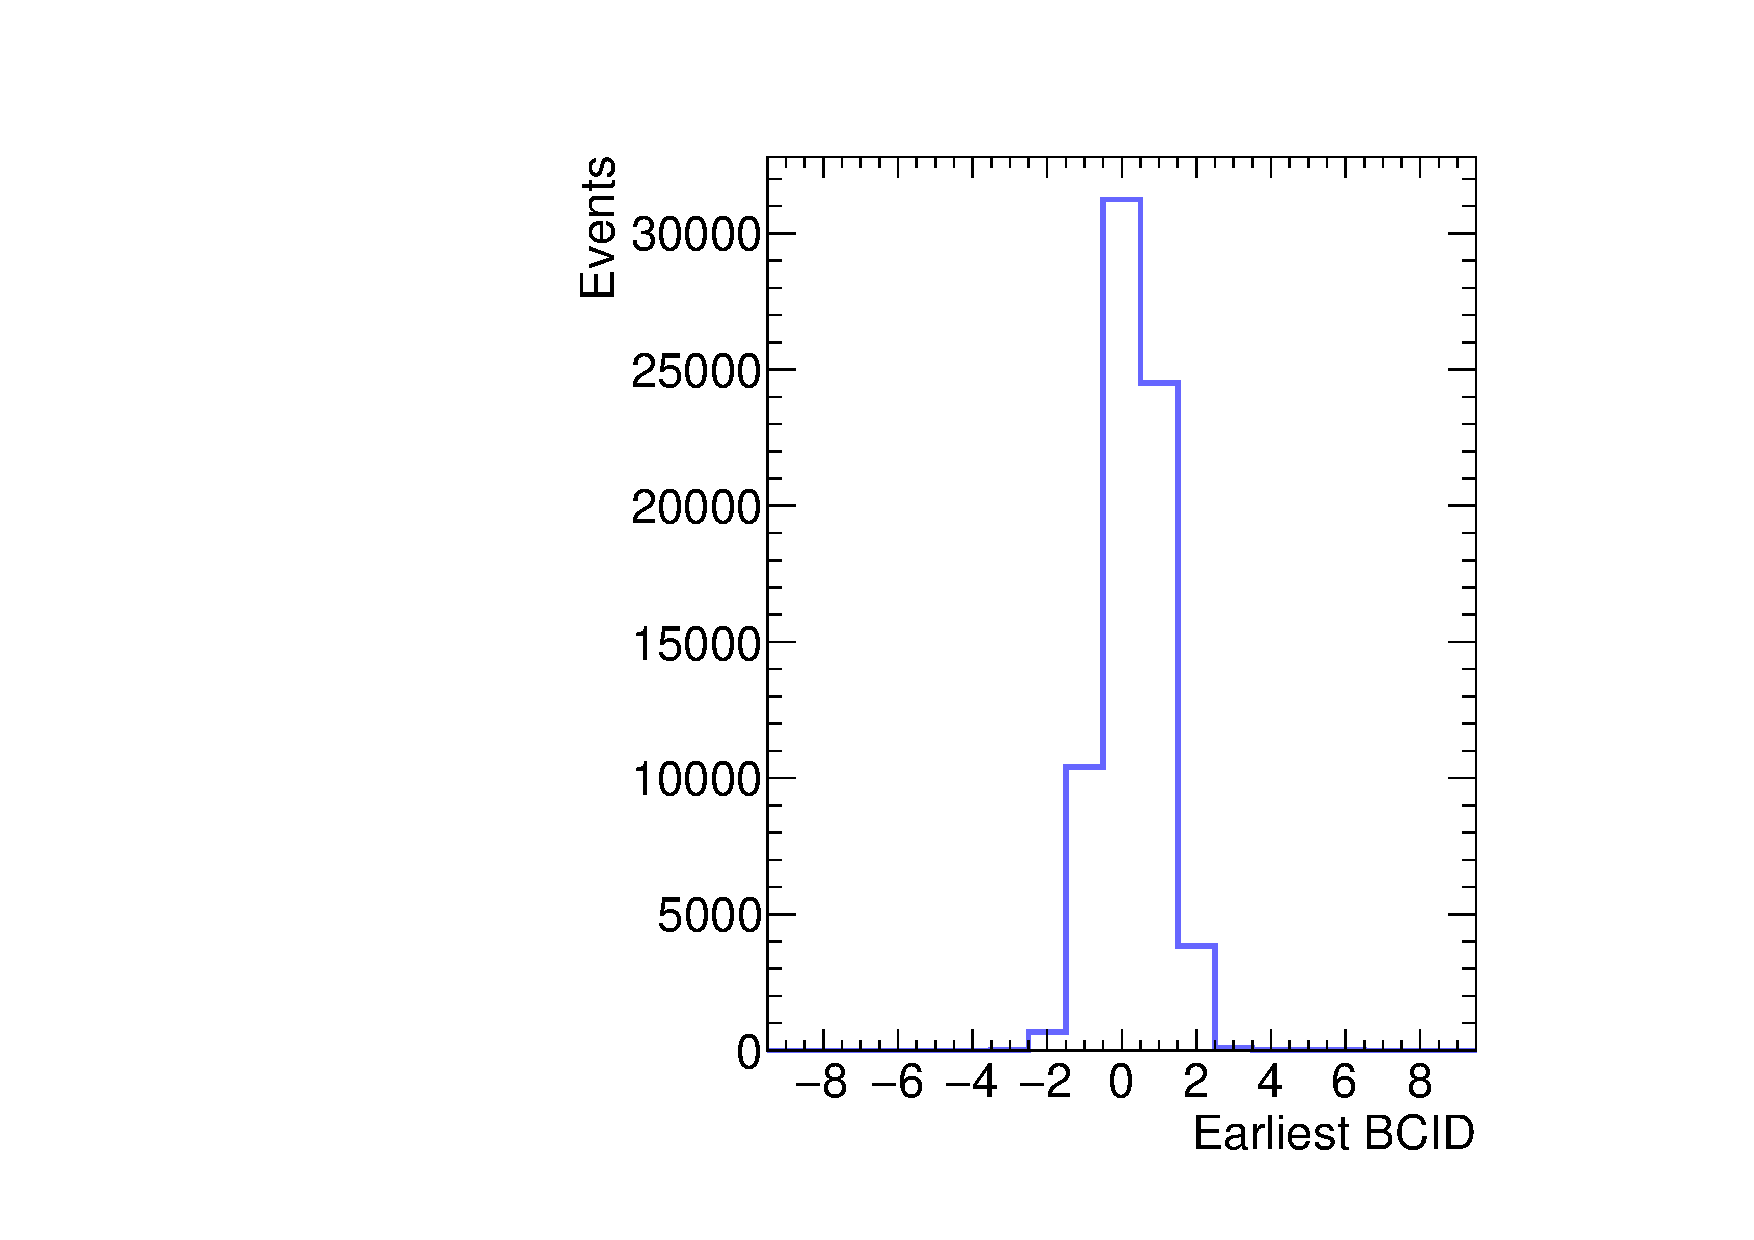
\includegraphics[width=0.3\textwidth]{figures/gbtanalysis3528/earliest_BCID.pdf}
  \end{center}
  \vspace{-10pt}
  \caption{
Distributions of the BCID difference between the scintillator trigger and the MMTP trigger
 for all events collected with (left) 200, (center) 100, and  (right) 50 ns peaktime.
 The MMTP  time is evaluated as as the BCID of the earliest ART hit.}
  \label{fig:integ_avg_earliest}
\end{figure}
%%%%%%%%%%%%%%%%%%%%%%%%%%%%%%%%%%%%%%%%%%%%%%%%%%%%%%%%%

 We use a Monte Carlo simulation to evaluate the efficiency of the MMTP algorithm as a function of the BC window
 for different peaktime. The result is shown in Fig. \ref{fig:peakeff}.
%%%%%%%%%%%%%%%%%%%%%%%%%%%%%%%%%%%%%%%%%%%%%%%%%%%%%%%%%%
\begin{figure}[!htpb]
  \begin{center}
    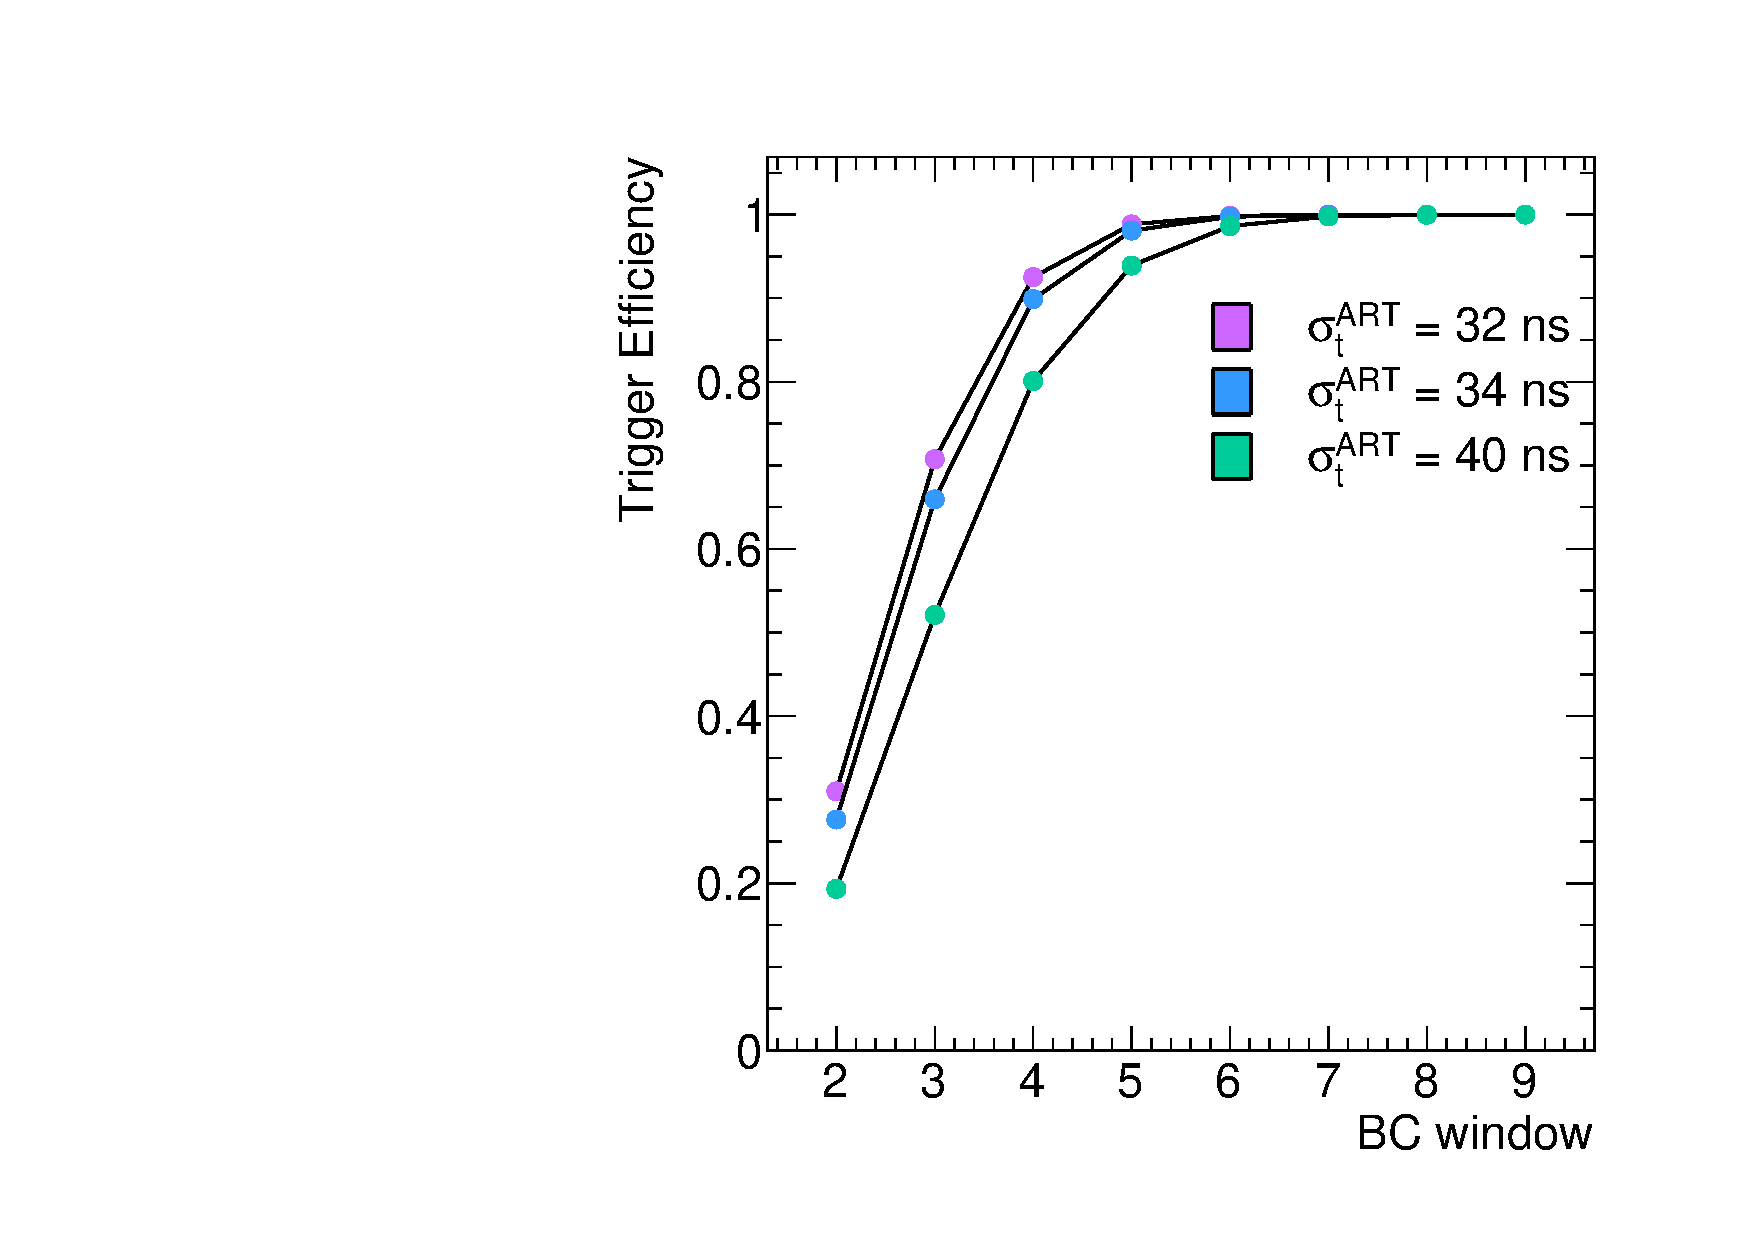
\includegraphics[width=0.8\textwidth]{figures/trigeffs.pdf}
\end{center}
  \vspace{-10pt}
  \caption{ Simulated efficiency of the MMTP algorithm as a function of the BC window for different peaktimes.
 This estimate is based on an octuplet with 100\% efficiency.}
  \label{fig:peakeff}
\end{figure}
%%%%%%%%%%%%%%%%%%%%%%%%%%%%%%%%%%%%%%%%%%%%%%%%%%%%%%%%%

